% Webinar 4 of the Idiot Brain series (Armenian): chapter 5, "Did you see this chapter coming?" (perception).
% Build from the repo root (queued behind the other decks' builds; one pass ~3 min, --full ~10-17 min):
%     python 02_idiot_brain/slides/common/build_deck.py webinar04 --full
% Needs the art first: uv run 02_idiot_brain/slides/common/build_art.py
% Speaker notes: NOTES.md (by frame number and title). ~95 min talk incl. a 5 min break.
\documentclass[aspectratio=169,11pt]{beamer}
% =====================================================================
%  The Idiot Brain webinars - shared Beamer preamble (the banner look)
% ---------------------------------------------------------------------
%  Usage (in slides/webinarNN/webinarNN.tex):
%      \documentclass[aspectratio=169,11pt]{beamer}
%      % =====================================================================
%  The Idiot Brain webinars - shared Beamer preamble (the banner look)
% ---------------------------------------------------------------------
%  Usage (in slides/webinarNN/webinarNN.tex):
%      \documentclass[aspectratio=169,11pt]{beamer}
%      % =====================================================================
%  The Idiot Brain webinars - shared Beamer preamble (the banner look)
% ---------------------------------------------------------------------
%  Usage (in slides/webinarNN/webinarNN.tex):
%      \documentclass[aspectratio=169,11pt]{beamer}
%      \input{../common/preamble.tex}
%  Build from the deck folder:  latexmk -lualatex -outdir=build webinarNN.tex
%  Art (emoji, mascot moods, title banner) comes from common/build_art.py.
%
%  All styling lives here, so decks only hold content. Palette and fonts
%  are the banner's (banner/build_banner.py): plum text on cream, pastel
%  accents, Mardoto for text, Glazz for big titles, Twemoji icons and
%  the pink brain mascot (DECISIONS.md #4-#6).
% =====================================================================

% ---------------------------------------------------------------------
% Fonts (LuaLaTeX + fontspec), shared with the banner
% ---------------------------------------------------------------------
\usepackage{fontspec}
\tracinglostchars=3 % a glyph missing from a font stops the build instead of printing nothing
\defaultfontfeatures{Ligatures=TeX}
\def\idiotfontdir{../../banner/assets/fonts/}
\setsansfont{Mardoto}[Path=\idiotfontdir, Extension=.ttf, UprightFont=*-Regular, BoldFont=*-Bold]
\setmainfont{Mardoto}[Path=\idiotfontdir, Extension=.ttf, UprightFont=*-Regular, BoldFont=*-Bold]
\newfontfamily\mediumfont{Mardoto-Medium}[Path=\idiotfontdir, Extension=.ttf]
\newfontfamily\blackfont{Mardoto-Black}[Path=\idiotfontdir, Extension=.ttf]
\newfontfamily\titlefont{GlazzArm-Regular}[Path=\idiotfontdir, Extension=.ttf] % Armenian letters only
\newfontfamily\handfont{Ink Free} % Windows font with Armenian; speech bubbles only
% Mardoto has no italic: emphasis is medium weight in the accent colour instead.
\renewcommand{\emph}[1]{{\mediumfont\color{plum}#1}}
% No hyphenation: split words are hard to read on a shared screen.
\hyphenpenalty=10000
\exhyphenpenalty=10000

% ---------------------------------------------------------------------
% Packages
% ---------------------------------------------------------------------
\usepackage{graphicx}
\usepackage{booktabs}
\usepackage[most]{tcolorbox}
\usepackage{tikz}
\usetikzlibrary{arrows.meta, positioning, calc, shapes.geometric, shapes.callouts, shapes.misc,
  decorations.pathmorphing, decorations.pathreplacing, backgrounds, fit, patterns.meta}
\usepackage{pgfplots}
\pgfplotsset{compat=1.18}
\usepgfplotslibrary{fillbetween}
\graphicspath{{../common/art/}{images/}}

% ---------------------------------------------------------------------
% Colours: the banner palette. Charts with 3+ series use the Armenian
% flag colours (amRed / amBlue / amOrange).
% ---------------------------------------------------------------------
\definecolor{plum}{HTML}{4A2340}
\definecolor{brainpink}{HTML}{F7A8C4}
\definecolor{fold}{HTML}{E57FA6}
\definecolor{cream}{HTML}{FFF6EC}
\definecolor{cardwhite}{HTML}{FFFDF9}
\definecolor{peach}{HTML}{FFD9C2}
\definecolor{lavender}{HTML}{D9C8F5}
\definecolor{mint}{HTML}{B5E8D5}
\definecolor{butter}{HTML}{FFE8A3}
\definecolor{blush}{HTML}{FF8FA8}
\definecolor{amRed}{HTML}{D90012}
\definecolor{amBlue}{HTML}{0033A0}
\definecolor{amOrange}{HTML}{F2A800}
% darker partners for text on cream
\colorlet{mintdark}{mint!45!black!80!green}
\definecolor{mintdark}{HTML}{2E7D62}
\definecolor{lavenderdark}{HTML}{5B3FA0}
\definecolor{peachdark}{HTML}{B5532A}
\definecolor{pinkdark}{HTML}{C2185B}
% names used by the figure files
\colorlet{ink}{plum}
\colorlet{paper}{cream}
\colorlet{mist}{lavender!40!cream}
\definecolor{night}{HTML}{2B2150}
\colorlet{softgray}{plum!60!cream}
% accent of the current part; \partaccent{<colour>} switches it
\colorlet{accent}{butter}
\newcommand{\partaccent}[1]{\colorlet{accent}{#1}}

% ---------------------------------------------------------------------
% Art: \emoji, \mascot (pages of common/art/*.pdf, see build_art.py)
% ---------------------------------------------------------------------
\makeatletter
\newcommand{\artpage}[3]{\expandafter\def\csname idiot@art@#1@#2\endcsname{#3}}
\input{../common/art/art_index.tex}
\newcommand{\idiot@art}[3]{% kind, name, size options
  \ifcsname idiot@art@#1@#2\endcsname
    \includegraphics[#3, page=\csname idiot@art@#1@#2\endcsname]{#1.pdf}%
  \else
    \PackageError{idiot}{Unknown #1 '#2'; add it to build_art.py and rebuild the art}{}%
  \fi}
% \emoji[<height>]{name}: inline icon, sits on the text baseline like a letter
\newcommand{\emoji}[2][1.15em]{\raisebox{-0.2em}{\idiot@art{emoji}{#2}{height=#1}}}
% \bigemoji[<height>]{name}: no baseline shift, for TikZ nodes and big pictures
\newcommand{\bigemoji}[2][1.5cm]{\idiot@art{emoji}{#2}{height=#1}}
% \mascot[<width>]{mood}: panic, happy, scared, sleepy, sick, confused, smug, hungry, thinking
\newcommand{\mascot}[2][2.6cm]{\idiot@art{mascot}{#2}{width=#1}}
\makeatother
% the older figure files place the mascot with \pic{noggin=<mood>}
\tikzset{pics/noggin/.style={code={\node[inner sep=0, transform shape] {\mascot[2.7cm]{#1}};}}}

% ---------------------------------------------------------------------
% Beamer look
% ---------------------------------------------------------------------
\setbeamertemplate{navigation symbols}{}
\setbeamercolor{normal text}{fg=plum, bg=cream}
\setbeamercolor{structure}{fg=plum}
\setbeamercolor{alerted text}{fg=pinkdark}
\setbeamerfont{alerted text}{series=\bfseries}
\setbeamercolor{frametitle}{fg=plum}
\setbeamersize{text margin left=9mm, text margin right=9mm}
\setbeamertemplate{frame begin}{\raggedright} % justified Armenian leaves big gaps

% cream paper with the banner's faint dot grid
\setbeamertemplate{background}{%
  \begin{tikzpicture}
    \fill[cream] (0,0) rectangle (\paperwidth,\paperheight);
    \fill[pattern={Dots[distance=4.4mm, radius=0.28mm]}, pattern color=plum!9!cream]
      (0,0) rectangle (\paperwidth,\paperheight);
  \end{tikzpicture}}

% topic pill, top right of every frame: set by \topic (emoji + short name)
\def\idiottopicemoji{}
\def\idiottopicname{}
\newcommand{\idiotpill}[3][cardwhite]{% fill, emoji, text
  \tikz[baseline=(p.base)]{\node[fill=#1, draw=plum, line width=0.7pt, rounded corners=2.6mm,
      inner xsep=2.2mm, inner ysep=1.1mm, font=\mediumfont\footnotesize, text=plum] (p)
      {\ifx\relax#2\relax\else\emoji[1.05em]{#2}\hspace{1.2mm}\fi#3};
    \begin{scope}[on background layer]
      \fill[plum, rounded corners=2.6mm] ([xshift=0.7mm, yshift=-0.7mm]p.south west) rectangle ([xshift=0.7mm, yshift=-0.7mm]p.north east);
    \end{scope}}}
% \chip{emoji}{text}: inline sticker label, same as the banner's topic chips
\newcommand{\chip}[3][cardwhite]{\idiotpill[#1]{#2}{#3}}

\setbeamertemplate{frametitle}{%
  \vskip 3.5mm
  \begin{minipage}[t]{0.66\paperwidth}
    \raggedright{\blackfont\fontsize{17.5}{20.5}\selectfont\insertframetitle}\par
    \vskip 1.3mm
    \tikz\fill[accent, rounded corners=0.6mm] (0,0) rectangle (1.5cm,1.1mm);
  \end{minipage}%
  \hfill
  \ifx\idiottopicname\empty\else
    \raisebox{-1mm}{\idiotpill{\idiottopicemoji}{\idiottopicname}}%
  \fi
  \vskip 1mm}

\setbeamertemplate{footline}{%
  \hbox to \paperwidth{\hskip 9mm
    {\mediumfont\fontsize{7}{8}\selectfont\color{plum!55!cream}Ապուշ ուղեղը · \insertshorttitle}\hfill
    {\blackfont\fontsize{8}{9}\selectfont\color{plum!70!cream}\insertframenumber}\hskip 9mm}
  \vskip 3mm}

\setbeamertemplate{itemize item}{\tikz[baseline=-0.65ex]\draw[plum, fill=accent, line width=0.6pt] (0,0) circle (0.95mm);}
\setbeamertemplate{itemize subitem}{\tikz[baseline=-0.65ex]\fill[plum!70] (0,0) circle (0.6mm);}
\setbeamertemplate{enumerate item}{\tikz[baseline=(n.base)]\node[fill=accent, draw=plum, line width=0.6pt,
  circle, inner sep=0.5mm, minimum size=4.2mm, font=\blackfont\scriptsize] (n) {\insertenumlabel};}
\setlength{\leftmargini}{5mm}
\setbeamertemplate{itemize/enumerate body begin}{\setlength{\itemsep}{1.6mm}}
\setbeamertemplate{itemize/enumerate subbody begin}{\setlength{\itemsep}{0.6mm}\small}

% ---------------------------------------------------------------------
% Structure: parts (full-colour openers) and topics (book sections)
% ---------------------------------------------------------------------
% \topic{<emoji>}{<short name>}: starts a book section; the pill shows on every following frame
\newcommand{\topic}[2]{\subsection{#2}\gdef\idiottopicemoji{#1}\gdef\idiottopicname{#2}}
\newcommand{\notopic}{\gdef\idiottopicemoji{}\gdef\idiottopicname{}}

% \partopener{<label>}{<title>}{<subtitle>}{<mood>}{<colour>}
\newcommand{\partopener}[5]{%
  \section{#2}\notopic\partaccent{#5}%
  \begin{frame}[plain]
    \begin{tikzpicture}[remember picture, overlay]
      \fill[#5] (current page.south west) rectangle (current page.north east);
      \fill[pattern={Dots[distance=4.4mm, radius=0.28mm]}, pattern color=plum!12!#5]
        (current page.south west) rectangle (current page.north east);
      \fill[cardwhite, opacity=0.45] ([xshift=-3.3cm, yshift=-0.2cm]current page.east) circle (3.1cm);
      \node[anchor=north west, inner sep=0] at ([xshift=10mm, yshift=-12mm]current page.north west)
        {\idiotpill{}{#1}};
      \node[anchor=west, text=plum, align=left, text width=9.2cm, inner sep=0]
        (t) at ([xshift=10mm, yshift=5mm]current page.west)
        {\titlefont\fontsize{38}{40}\selectfont #2};
      \node[anchor=north west, text=plum, text width=9.2cm, inner sep=0, align=left]
        at ([yshift=-5mm]t.south west) {\mediumfont\large #3};
      \node at ([xshift=-3.3cm, yshift=-0.2cm]current page.east) {\mascot[4.6cm]{#4}};
    \end{tikzpicture}
  \end{frame}}

% \topicopener{<emoji>}{<short name>}{<book's section title>}{<what it is about>}{<mood>}
\newcommand{\topicopener}[5]{%
  \topic{#1}{#2}%
  \begin{frame}[plain]
    \begin{tikzpicture}[remember picture, overlay]
      \fill[accent!55!cream] (current page.south west) rectangle (current page.north east);
      \fill[pattern={Dots[distance=4.4mm, radius=0.28mm]}, pattern color=plum!10!accent!55!cream]
        (current page.south west) rectangle (current page.north east);
      \node[anchor=north west, inner sep=0] at ([xshift=10mm, yshift=-12mm]current page.north west)
        {\idiotpill{#1}{#2}};
      \node[anchor=west, text=plum, text width=9.6cm, align=left, inner sep=0]
        (t) at ([xshift=10mm, yshift=6mm]current page.west)
        {\blackfont\fontsize{24}{28}\selectfont «#3»};
      \node[anchor=north west, text=plum, text width=9.6cm, align=left, inner sep=0]
        at ([yshift=-4mm]t.south west) {\mediumfont\large #4};
      \node at ([xshift=-3.0cm, yshift=-0.4cm]current page.east) {\mascot[4.2cm]{#5}};
      \node[rotate=-12] at ([xshift=-1.4cm, yshift=2.3cm]current page.east) {\bigemoji[1.5cm]{#1}};
    \end{tikzpicture}
  \end{frame}}

% ---------------------------------------------------------------------
% Boxes (sticker style: plum outline + hard plum shadow, like the banner)
% ---------------------------------------------------------------------
\tcbset{
  sticker/.style={enhanced, arc=3mm, boxrule=0.9pt, colframe=plum, colback=cardwhite, halign=left,
    left=3mm, right=3mm, top=2mm, bottom=2mm, fontupper=\normalsize, coltext=plum,
    shadow={1.1mm}{-1.1mm}{0mm}{fill=plum}},
  tagged/.style={sticker, colback=#1!45!cream, colbacktitle=#1, coltitle=plum,
    fonttitle=\blackfont\footnotesize, top=3mm,
    attach boxed title to top left={xshift=4mm, yshift*=-2.4mm},
    boxed title style={arc=2.2mm, boxrule=0.9pt, colframe=plum, left=1.5mm, right=1.5mm, top=0.6mm, bottom=0.6mm}},
}
\newtcolorbox{card}[1][]{sticker, #1}
\newtcolorbox{tryit}[1][]{tagged=mint, title={\emoji[1em]{testtube}\ Փորձիր հիմա}, #1}
\newtcolorbox{poll}[1][]{tagged=butter, title={\emoji[1em]{hand}\ Հարցում}, #1}
\newtcolorbox{chatbox}[1][]{tagged=lavender, title={\emoji[1em]{speech}\ Գրիր չաթում}, #1}
\newtcolorbox{scienceupdate}[1][]{tagged=peach, fontupper=\small, title={\emoji[1em]{microscope}\ Գիտությունն այսօր}, #1}
\newtcolorbox{bookquote}[1][]{sticker, colback=cardwhite, fontupper=\mediumfont, left=4mm,
  borderline west={1.4mm}{0pt}{accent},
  before upper={{\blackfont\footnotesize\emoji[1em]{book}\ Բըրնեթը գրում է}\par\smallskip}, #1}

% Brain.exe-style popup window: \begin{popup}{<window title>} ... \end{popup}
\newcommand{\winbuttons}{%
  \tikz[baseline=-0.6ex, line width=0.6pt]{
    \foreach \i/\f in {0/cardwhite, 1/cardwhite, 2/blush}{
      \filldraw[fill=\f, draw=plum, rounded corners=0.6mm] (\i*4.3mm,-1.6mm) rectangle ++(3.3mm,3.3mm);}
    \draw[plum] (0.8mm,-0.8mm) -- (2.5mm,-0.8mm);
    \draw[plum] (5.1mm,-0.8mm) rectangle (6.8mm,0.9mm);
    \draw[plum] (9.4mm,-0.9mm) -- (11.1mm,0.8mm) (9.4mm,0.8mm) -- (11.1mm,-0.9mm);}}
\newtcolorbox{popup}[2][]{sticker, colback=cardwhite, colbacktitle=brainpink, coltitle=plum,
  fonttitle=\blackfont\small, title={\emoji[1.1em]{warning}\hspace{1.5mm}#2\hfill\winbuttons},
  titlerule=0.9pt, toptitle=0.8mm, bottomtitle=0.8mm, #1}

% Myth or fact: \mythorfact{<statement>}{<verdict>}{<colour>}{<explanation>}; verdict shows on slide 2
\newcommand{\mythorfact}[4]{%
  \begin{center}
  \begin{tikzpicture}
    \node[draw=plum, line width=0.9pt, fill=cardwhite, rounded corners=4mm, inner xsep=8mm, inner ysep=6mm,
          text width=10cm, align=center, font=\blackfont\Large, text=plum] (mf) {«#1»};
    \begin{scope}[on background layer]
      \fill[plum, rounded corners=4mm] ([xshift=1.2mm, yshift=-1.2mm]mf.south west) rectangle ([xshift=1.2mm, yshift=-1.2mm]mf.north east);
    \end{scope}
    \node[anchor=west] at ([xshift=6mm]mf.north west) {\idiotpill[butter]{question}{Առասպել, թե՞ փաստ}};
    \onslide<2->{\node[draw=#3, text=#3, line width=2pt, rounded corners=2mm, rotate=-10, font=\blackfont\LARGE,
      inner sep=4pt, fill=cardwhite] at ([xshift=-8mm, yshift=1mm]mf.south east) {#2};}
  \end{tikzpicture}
  \end{center}
  \onslide<2->{#4}}

% Big question with the confused mascot: \bigquestion{<question>}{<small line>}
\newcommand{\bigquestion}[2]{%
  \vfill
  \begin{center}
  \begin{tikzpicture}
    \node[text width=9.6cm, align=center, font=\blackfont\fontsize{24}{29}\selectfont, text=plum] (q) {#1};
    \node[below=4mm of q, text width=9.6cm, align=center, font=\mediumfont\large, text=softgray] {#2};
    \node[anchor=east] at ([xshift=-2mm]q.west) {\mascot[2.6cm]{confused}};
  \end{tikzpicture}
  \end{center}
  \vfill}

% Small source line at the bottom of a frame: \source{Loftus & Palmer, 1974}
\newcommand{\source}[1]{%
  \begin{tikzpicture}[remember picture, overlay]
    \node[anchor=south east, font=\fontsize{6.5}{7.5}\selectfont, text=plum!60!cream, inner sep=0]
      at ([xshift=-17mm, yshift=3.4mm]current page.south east) {Աղբյուր՝ #1};
  \end{tikzpicture}}

% Speech bubbles (handwritten) and the overlay helper for TikZ:
% \node[visible on=<2->] ... keeps the layout but hides the node until slide 2.
\tikzset{
  say/.style={rectangle callout, draw=plum, line width=0.8pt, fill=cardwhite, rounded corners=3pt,
    inner sep=4pt, align=center, font=\handfont\normalsize, text=plum},
  think/.style={cloud callout, cloud puffs=12, draw=plum, line width=0.8pt, fill=cardwhite,
    inner sep=2pt, align=center, font=\handfont\normalsize, text=plum},
  % boxes for diagrams drawn directly in a frame: a style with #1 cannot be defined inside a frame body
  flow/.style={draw=plum, line width=0.8pt, fill=cardwhite, rounded corners=2mm, align=center,
    font=\small, text=plum, inner sep=4pt, text width=#1},
  flow/.default=3cm,
  chatmsg/.style={draw=plum, line width=0.8pt, rounded corners=3mm, inner sep=6pt, text width=#1,
    align=left, font=\small, text=plum},
  chatmsg/.default=7cm,
  invisible/.style={opacity=0, text opacity=0},
  visible on/.style={alt={#1{}{invisible}}},
  alt/.code args={<#1>#2#3}{\alt<#1>{\pgfkeysalso{#2}}{\pgfkeysalso{#3}}},
}

%  Build from the deck folder:  latexmk -lualatex -outdir=build webinarNN.tex
%  Art (emoji, mascot moods, title banner) comes from common/build_art.py.
%
%  All styling lives here, so decks only hold content. Palette and fonts
%  are the banner's (banner/build_banner.py): plum text on cream, pastel
%  accents, Mardoto for text, Glazz for big titles, Twemoji icons and
%  the pink brain mascot (DECISIONS.md #4-#6).
% =====================================================================

% ---------------------------------------------------------------------
% Fonts (LuaLaTeX + fontspec), shared with the banner
% ---------------------------------------------------------------------
\usepackage{fontspec}
\tracinglostchars=3 % a glyph missing from a font stops the build instead of printing nothing
\defaultfontfeatures{Ligatures=TeX}
\def\idiotfontdir{../../banner/assets/fonts/}
\setsansfont{Mardoto}[Path=\idiotfontdir, Extension=.ttf, UprightFont=*-Regular, BoldFont=*-Bold]
\setmainfont{Mardoto}[Path=\idiotfontdir, Extension=.ttf, UprightFont=*-Regular, BoldFont=*-Bold]
\newfontfamily\mediumfont{Mardoto-Medium}[Path=\idiotfontdir, Extension=.ttf]
\newfontfamily\blackfont{Mardoto-Black}[Path=\idiotfontdir, Extension=.ttf]
\newfontfamily\titlefont{GlazzArm-Regular}[Path=\idiotfontdir, Extension=.ttf] % Armenian letters only
\newfontfamily\handfont{Ink Free} % Windows font with Armenian; speech bubbles only
% Mardoto has no italic: emphasis is medium weight in the accent colour instead.
\renewcommand{\emph}[1]{{\mediumfont\color{plum}#1}}
% No hyphenation: split words are hard to read on a shared screen.
\hyphenpenalty=10000
\exhyphenpenalty=10000

% ---------------------------------------------------------------------
% Packages
% ---------------------------------------------------------------------
\usepackage{graphicx}
\usepackage{booktabs}
\usepackage[most]{tcolorbox}
\usepackage{tikz}
\usetikzlibrary{arrows.meta, positioning, calc, shapes.geometric, shapes.callouts, shapes.misc,
  decorations.pathmorphing, decorations.pathreplacing, backgrounds, fit, patterns.meta}
\usepackage{pgfplots}
\pgfplotsset{compat=1.18}
\usepgfplotslibrary{fillbetween}
\graphicspath{{../common/art/}{images/}}

% ---------------------------------------------------------------------
% Colours: the banner palette. Charts with 3+ series use the Armenian
% flag colours (amRed / amBlue / amOrange).
% ---------------------------------------------------------------------
\definecolor{plum}{HTML}{4A2340}
\definecolor{brainpink}{HTML}{F7A8C4}
\definecolor{fold}{HTML}{E57FA6}
\definecolor{cream}{HTML}{FFF6EC}
\definecolor{cardwhite}{HTML}{FFFDF9}
\definecolor{peach}{HTML}{FFD9C2}
\definecolor{lavender}{HTML}{D9C8F5}
\definecolor{mint}{HTML}{B5E8D5}
\definecolor{butter}{HTML}{FFE8A3}
\definecolor{blush}{HTML}{FF8FA8}
\definecolor{amRed}{HTML}{D90012}
\definecolor{amBlue}{HTML}{0033A0}
\definecolor{amOrange}{HTML}{F2A800}
% darker partners for text on cream
\colorlet{mintdark}{mint!45!black!80!green}
\definecolor{mintdark}{HTML}{2E7D62}
\definecolor{lavenderdark}{HTML}{5B3FA0}
\definecolor{peachdark}{HTML}{B5532A}
\definecolor{pinkdark}{HTML}{C2185B}
% names used by the figure files
\colorlet{ink}{plum}
\colorlet{paper}{cream}
\colorlet{mist}{lavender!40!cream}
\definecolor{night}{HTML}{2B2150}
\colorlet{softgray}{plum!60!cream}
% accent of the current part; \partaccent{<colour>} switches it
\colorlet{accent}{butter}
\newcommand{\partaccent}[1]{\colorlet{accent}{#1}}

% ---------------------------------------------------------------------
% Art: \emoji, \mascot (pages of common/art/*.pdf, see build_art.py)
% ---------------------------------------------------------------------
\makeatletter
\newcommand{\artpage}[3]{\expandafter\def\csname idiot@art@#1@#2\endcsname{#3}}
% generated by build_art.py - do not edit
\artpage{emoji}{brain}{1}
\artpage{emoji}{warning}{2}
\artpage{emoji}{rollercoaster}{3}
\artpage{emoji}{doughnut}{4}
\artpage{emoji}{sleeping}{5}
\artpage{emoji}{scream}{6}
\artpage{emoji}{thought}{7}
\artpage{emoji}{question}{8}
\artpage{emoji}{cyclone}{9}
\artpage{emoji}{calendar}{10}
\artpage{emoji}{clock630}{11}
\artpage{emoji}{computer}{12}
\artpage{emoji}{receipt}{13}
\artpage{emoji}{gift}{14}
\artpage{emoji}{lizard}{15}
\artpage{emoji}{boss}{16}
\artpage{emoji}{keyboard}{17}
\artpage{emoji}{wastebasket}{18}
\artpage{emoji}{batterylow}{19}
\artpage{emoji}{skull}{20}
\artpage{emoji}{car}{21}
\artpage{emoji}{ship}{22}
\artpage{emoji}{airplane}{23}
\artpage{emoji}{nauseated}{24}
\artpage{emoji}{vomit}{25}
\artpage{emoji}{eye}{26}
\artpage{emoji}{ear}{27}
\artpage{emoji}{tree}{28}
\artpage{emoji}{wave}{29}
\artpage{emoji}{book}{30}
\artpage{emoji}{walking}{31}
\artpage{emoji}{dizzy}{32}
\artpage{emoji}{cake}{33}
\artpage{emoji}{icecream}{34}
\artpage{emoji}{potato}{35}
\artpage{emoji}{apple}{36}
\artpage{emoji}{burger}{37}
\artpage{emoji}{salad}{38}
\artpage{emoji}{clock12}{39}
\artpage{emoji}{forkknife}{40}
\artpage{emoji}{pasta}{41}
\artpage{emoji}{fire}{42}
\artpage{emoji}{drool}{43}
\artpage{emoji}{pizza}{44}
\artpage{emoji}{bed}{45}
\artpage{emoji}{personbed}{46}
\artpage{emoji}{moon}{47}
\artpage{emoji}{sun}{48}
\artpage{emoji}{zzz}{49}
\artpage{emoji}{dolphin}{50}
\artpage{emoji}{jellyfish}{51}
\artpage{emoji}{rat}{52}
\artpage{emoji}{chipmunk}{53}
\artpage{emoji}{alarm}{54}
\artpage{emoji}{phone}{55}
\artpage{emoji}{ghost}{56}
\artpage{emoji}{alien}{57}
\artpage{emoji}{yawn}{58}
\artpage{emoji}{baby}{59}
\artpage{emoji}{construction}{60}
\artpage{emoji}{broom}{61}
\artpage{emoji}{thermometer}{62}
\artpage{emoji}{cold}{63}
\artpage{emoji}{monkey}{64}
\artpage{emoji}{tiger}{65}
\artpage{emoji}{axe}{66}
\artpage{emoji}{balloon}{67}
\artpage{emoji}{heart}{68}
\artpage{emoji}{anatomicalheart}{69}
\artpage{emoji}{lungs}{70}
\artpage{emoji}{sweat}{71}
\artpage{emoji}{eyes}{72}
\artpage{emoji}{butterfly}{73}
\artpage{emoji}{runner}{74}
\artpage{emoji}{boxing}{75}
\artpage{emoji}{station}{76}
\artpage{emoji}{taxi}{77}
\artpage{emoji}{bell}{78}
\artpage{emoji}{couch}{79}
\artpage{emoji}{muscle}{80}
\artpage{emoji}{toilet}{81}
\artpage{emoji}{floppy}{82}
\artpage{emoji}{door}{83}
\artpage{emoji}{coffee}{84}
\artpage{emoji}{diving}{85}
\artpage{emoji}{wine}{86}
\artpage{emoji}{beer}{87}
\artpage{emoji}{dove}{88}
\artpage{emoji}{puzzle}{89}
\artpage{emoji}{fish}{90}
\artpage{emoji}{trophy}{91}
\artpage{emoji}{detective}{92}
\artpage{emoji}{judge}{93}
\artpage{emoji}{cheese}{94}
\artpage{emoji}{film}{95}
\artpage{emoji}{magnifier}{96}
\artpage{emoji}{key}{97}
\artpage{emoji}{firework}{98}
\artpage{emoji}{house}{99}
\artpage{emoji}{gloves}{100}
\artpage{emoji}{trafficlight}{101}
\artpage{emoji}{stop}{102}
\artpage{emoji}{mute}{103}
\artpage{emoji}{videogame}{104}
\artpage{emoji}{mirror}{105}
\artpage{emoji}{star}{106}
\artpage{emoji}{hospital}{107}
\artpage{emoji}{pill}{108}
\artpage{emoji}{camera}{109}
\artpage{emoji}{tv}{110}
\artpage{emoji}{crown}{111}
\artpage{emoji}{nerd}{112}
\artpage{emoji}{lock}{113}
\artpage{emoji}{musical}{114}
\artpage{emoji}{chips}{115}
\artpage{emoji}{check}{116}
\artpage{emoji}{cross}{117}
\artpage{emoji}{hand}{118}
\artpage{emoji}{wavehand}{119}
\artpage{emoji}{speech}{120}
\artpage{emoji}{pencil}{121}
\artpage{emoji}{memo}{122}
\artpage{emoji}{monocle}{123}
\artpage{emoji}{thinking}{124}
\artpage{emoji}{grin}{125}
\artpage{emoji}{sweatsmile}{126}
\artpage{emoji}{facepalm}{127}
\artpage{emoji}{popcorn}{128}
\artpage{emoji}{bulb}{129}
\artpage{emoji}{sparkles}{130}
\artpage{emoji}{party}{131}
\artpage{emoji}{chart}{132}
\artpage{emoji}{testtube}{133}
\artpage{emoji}{people}{134}
\artpage{emoji}{pin}{135}
\artpage{emoji}{hourglass}{136}
\artpage{emoji}{microscope}{137}
\artpage{emoji}{books}{138}
\artpage{emoji}{megaphone}{139}
\artpage{emoji}{student}{140}
\artpage{emoji}{zany}{141}
\artpage{emoji}{hundred}{142}
\artpage{emoji}{link}{143}
\artpage{emoji}{target}{144}
\artpage{emoji}{clover}{145}
\artpage{emoji}{ufo}{146}
\artpage{emoji}{spider}{147}
\artpage{emoji}{spiderweb}{148}
\artpage{emoji}{snake}{149}
\artpage{emoji}{microphone}{150}
\artpage{emoji}{clown}{151}
\artpage{emoji}{pumpkin}{152}
\artpage{emoji}{knife}{153}
\artpage{emoji}{bat}{154}
\artpage{emoji}{blackcat}{155}
\artpage{emoji}{crossedfingers}{156}
\artpage{emoji}{ladder}{157}
\artpage{emoji}{thumbsup}{158}
\artpage{emoji}{thumbsdown}{159}
\artpage{emoji}{rocket}{160}
\artpage{emoji}{satellite}{161}
\artpage{emoji}{newspaper}{162}
\artpage{emoji}{chocolate}{163}
\artpage{emoji}{syringe}{164}
\artpage{emoji}{dice}{165}
\artpage{emoji}{hauntedhouse}{166}
\artpage{emoji}{flushed}{167}
\artpage{emoji}{fearful}{168}
\artpage{emoji}{graduation}{169}
\artpage{emoji}{teacher}{170}
\artpage{emoji}{scientist}{171}
\artpage{emoji}{chess}{172}
\artpage{emoji}{abacus}{173}
\artpage{emoji}{ruler}{174}
\artpage{emoji}{jeans}{175}
\artpage{emoji}{glasses}{176}
\artpage{emoji}{dna}{177}
\artpage{emoji}{loudspeaker}{178}
\artpage{emoji}{speakinghead}{179}
\artpage{emoji}{seedling}{180}
\artpage{emoji}{weightlifter}{181}
\artpage{emoji}{giraffe}{182}
\artpage{emoji}{mouse}{183}
\artpage{emoji}{exploding}{184}
\artpage{emoji}{owl}{185}
\artpage{emoji}{clipboard}{186}
\artpage{emoji}{numbers}{187}
\artpage{emoji}{medal}{188}
\artpage{emoji}{rose}{189}
\artpage{emoji}{nose}{190}
\artpage{emoji}{tongue}{191}
\artpage{emoji}{yum}{192}
\artpage{emoji}{bread}{193}
\artpage{emoji}{lemon}{194}
\artpage{emoji}{chili}{195}
\artpage{emoji}{salt}{196}
\artpage{emoji}{candy}{197}
\artpage{emoji}{speaker}{198}
\artpage{emoji}{headphones}{199}
\artpage{emoji}{feather}{200}
\artpage{emoji}{gorilla}{201}
\artpage{emoji}{basketball}{202}
\artpage{emoji}{magicwand}{203}
\artpage{emoji}{tophat}{204}
\artpage{emoji}{cloud}{205}
\artpage{emoji}{plug}{206}
\artpage{emoji}{clinking}{207}
\artpage{emoji}{dog}{208}
\artpage{emoji}{rainbow}{209}
\artpage{emoji}{slightsmile}{210}
\artpage{emoji}{palette}{211}
\artpage{emoji}{masks}{212}
\artpage{emoji}{angry}{213}
\artpage{emoji}{rage}{214}
\artpage{emoji}{steam}{215}
\artpage{emoji}{bomb}{216}
\artpage{emoji}{volcano}{217}
\artpage{emoji}{angersymbol}{218}
\artpage{emoji}{crystalball}{219}
\artpage{emoji}{railway}{220}
\artpage{emoji}{worker}{221}
\artpage{emoji}{laughing}{222}
\artpage{emoji}{rofl}{223}
\artpage{emoji}{banana}{224}
\artpage{emoji}{mountain}{225}
\artpage{emoji}{moneybag}{226}
\artpage{emoji}{lightning}{227}
\artpage{emoji}{joker}{228}
\artpage{emoji}{finishflag}{229}
\artpage{emoji}{hug}{230}
\artpage{emoji}{handshake}{231}
\artpage{emoji}{lying}{232}
\artpage{emoji}{neutral}{233}
\artpage{emoji}{carrot}{234}
\artpage{emoji}{wood}{235}
\artpage{emoji}{brokenheart}{236}
\artpage{emoji}{loveletter}{237}
\artpage{emoji}{couple}{238}
\artpage{emoji}{kiss}{239}
\artpage{emoji}{cowboy}{240}
\artpage{emoji}{guitar}{241}
\artpage{emoji}{family}{242}
\artpage{emoji}{police}{243}
\artpage{emoji}{sheep}{244}
\artpage{emoji}{clapping}{245}
\artpage{emoji}{imp}{246}
\artpage{emoji}{ballot}{247}
\artpage{emoji}{smileheart}{248}
\artpage{emoji}{dollar}{249}
\artpage{emoji}{earth}{250}
\artpage{emoji}{raincloud}{251}
\artpage{emoji}{sunbehindcloud}{252}
\artpage{emoji}{pensive}{253}
\artpage{emoji}{cry}{254}
\artpage{emoji}{bandage}{255}
\artpage{emoji}{stethoscope}{256}
\artpage{emoji}{cigarette}{257}
\artpage{emoji}{slotmachine}{258}
\artpage{emoji}{siren}{259}
\artpage{emoji}{sunrise}{260}
\artpage{emoji}{healthworker}{261}
\artpage{emoji}{hearnoevil}{262}
\artpage{emoji}{anchor}{263}
\artpage{emoji}{candle}{264}
\artpage{emoji}{telephone}{265}
\artpage{emoji}{battery}{266}
\artpage{emoji}{weary}{267}
\artpage{emoji}{lotus}{268}
\artpage{mascot}{panic}{1}
\artpage{mascot}{happy}{2}
\artpage{mascot}{scared}{3}
\artpage{mascot}{sleepy}{4}
\artpage{mascot}{sick}{5}
\artpage{mascot}{confused}{6}
\artpage{mascot}{smug}{7}
\artpage{mascot}{hungry}{8}
\artpage{mascot}{thinking}{9}
\artpage{mascot}{sad}{10}
\artpage{mascot}{angry}{11}

\newcommand{\idiot@art}[3]{% kind, name, size options
  \ifcsname idiot@art@#1@#2\endcsname
    \includegraphics[#3, page=\csname idiot@art@#1@#2\endcsname]{#1.pdf}%
  \else
    \PackageError{idiot}{Unknown #1 '#2'; add it to build_art.py and rebuild the art}{}%
  \fi}
% \emoji[<height>]{name}: inline icon, sits on the text baseline like a letter
\newcommand{\emoji}[2][1.15em]{\raisebox{-0.2em}{\idiot@art{emoji}{#2}{height=#1}}}
% \bigemoji[<height>]{name}: no baseline shift, for TikZ nodes and big pictures
\newcommand{\bigemoji}[2][1.5cm]{\idiot@art{emoji}{#2}{height=#1}}
% \mascot[<width>]{mood}: panic, happy, scared, sleepy, sick, confused, smug, hungry, thinking
\newcommand{\mascot}[2][2.6cm]{\idiot@art{mascot}{#2}{width=#1}}
\makeatother
% the older figure files place the mascot with \pic{noggin=<mood>}
\tikzset{pics/noggin/.style={code={\node[inner sep=0, transform shape] {\mascot[2.7cm]{#1}};}}}

% ---------------------------------------------------------------------
% Beamer look
% ---------------------------------------------------------------------
\setbeamertemplate{navigation symbols}{}
\setbeamercolor{normal text}{fg=plum, bg=cream}
\setbeamercolor{structure}{fg=plum}
\setbeamercolor{alerted text}{fg=pinkdark}
\setbeamerfont{alerted text}{series=\bfseries}
\setbeamercolor{frametitle}{fg=plum}
\setbeamersize{text margin left=9mm, text margin right=9mm}
\setbeamertemplate{frame begin}{\raggedright} % justified Armenian leaves big gaps

% cream paper with the banner's faint dot grid
\setbeamertemplate{background}{%
  \begin{tikzpicture}
    \fill[cream] (0,0) rectangle (\paperwidth,\paperheight);
    \fill[pattern={Dots[distance=4.4mm, radius=0.28mm]}, pattern color=plum!9!cream]
      (0,0) rectangle (\paperwidth,\paperheight);
  \end{tikzpicture}}

% topic pill, top right of every frame: set by \topic (emoji + short name)
\def\idiottopicemoji{}
\def\idiottopicname{}
\newcommand{\idiotpill}[3][cardwhite]{% fill, emoji, text
  \tikz[baseline=(p.base)]{\node[fill=#1, draw=plum, line width=0.7pt, rounded corners=2.6mm,
      inner xsep=2.2mm, inner ysep=1.1mm, font=\mediumfont\footnotesize, text=plum] (p)
      {\ifx\relax#2\relax\else\emoji[1.05em]{#2}\hspace{1.2mm}\fi#3};
    \begin{scope}[on background layer]
      \fill[plum, rounded corners=2.6mm] ([xshift=0.7mm, yshift=-0.7mm]p.south west) rectangle ([xshift=0.7mm, yshift=-0.7mm]p.north east);
    \end{scope}}}
% \chip{emoji}{text}: inline sticker label, same as the banner's topic chips
\newcommand{\chip}[3][cardwhite]{\idiotpill[#1]{#2}{#3}}

\setbeamertemplate{frametitle}{%
  \vskip 3.5mm
  \begin{minipage}[t]{0.66\paperwidth}
    \raggedright{\blackfont\fontsize{17.5}{20.5}\selectfont\insertframetitle}\par
    \vskip 1.3mm
    \tikz\fill[accent, rounded corners=0.6mm] (0,0) rectangle (1.5cm,1.1mm);
  \end{minipage}%
  \hfill
  \ifx\idiottopicname\empty\else
    \raisebox{-1mm}{\idiotpill{\idiottopicemoji}{\idiottopicname}}%
  \fi
  \vskip 1mm}

\setbeamertemplate{footline}{%
  \hbox to \paperwidth{\hskip 9mm
    {\mediumfont\fontsize{7}{8}\selectfont\color{plum!55!cream}Ապուշ ուղեղը · \insertshorttitle}\hfill
    {\blackfont\fontsize{8}{9}\selectfont\color{plum!70!cream}\insertframenumber}\hskip 9mm}
  \vskip 3mm}

\setbeamertemplate{itemize item}{\tikz[baseline=-0.65ex]\draw[plum, fill=accent, line width=0.6pt] (0,0) circle (0.95mm);}
\setbeamertemplate{itemize subitem}{\tikz[baseline=-0.65ex]\fill[plum!70] (0,0) circle (0.6mm);}
\setbeamertemplate{enumerate item}{\tikz[baseline=(n.base)]\node[fill=accent, draw=plum, line width=0.6pt,
  circle, inner sep=0.5mm, minimum size=4.2mm, font=\blackfont\scriptsize] (n) {\insertenumlabel};}
\setlength{\leftmargini}{5mm}
\setbeamertemplate{itemize/enumerate body begin}{\setlength{\itemsep}{1.6mm}}
\setbeamertemplate{itemize/enumerate subbody begin}{\setlength{\itemsep}{0.6mm}\small}

% ---------------------------------------------------------------------
% Structure: parts (full-colour openers) and topics (book sections)
% ---------------------------------------------------------------------
% \topic{<emoji>}{<short name>}: starts a book section; the pill shows on every following frame
\newcommand{\topic}[2]{\subsection{#2}\gdef\idiottopicemoji{#1}\gdef\idiottopicname{#2}}
\newcommand{\notopic}{\gdef\idiottopicemoji{}\gdef\idiottopicname{}}

% \partopener{<label>}{<title>}{<subtitle>}{<mood>}{<colour>}
\newcommand{\partopener}[5]{%
  \section{#2}\notopic\partaccent{#5}%
  \begin{frame}[plain]
    \begin{tikzpicture}[remember picture, overlay]
      \fill[#5] (current page.south west) rectangle (current page.north east);
      \fill[pattern={Dots[distance=4.4mm, radius=0.28mm]}, pattern color=plum!12!#5]
        (current page.south west) rectangle (current page.north east);
      \fill[cardwhite, opacity=0.45] ([xshift=-3.3cm, yshift=-0.2cm]current page.east) circle (3.1cm);
      \node[anchor=north west, inner sep=0] at ([xshift=10mm, yshift=-12mm]current page.north west)
        {\idiotpill{}{#1}};
      \node[anchor=west, text=plum, align=left, text width=9.2cm, inner sep=0]
        (t) at ([xshift=10mm, yshift=5mm]current page.west)
        {\titlefont\fontsize{38}{40}\selectfont #2};
      \node[anchor=north west, text=plum, text width=9.2cm, inner sep=0, align=left]
        at ([yshift=-5mm]t.south west) {\mediumfont\large #3};
      \node at ([xshift=-3.3cm, yshift=-0.2cm]current page.east) {\mascot[4.6cm]{#4}};
    \end{tikzpicture}
  \end{frame}}

% \topicopener{<emoji>}{<short name>}{<book's section title>}{<what it is about>}{<mood>}
\newcommand{\topicopener}[5]{%
  \topic{#1}{#2}%
  \begin{frame}[plain]
    \begin{tikzpicture}[remember picture, overlay]
      \fill[accent!55!cream] (current page.south west) rectangle (current page.north east);
      \fill[pattern={Dots[distance=4.4mm, radius=0.28mm]}, pattern color=plum!10!accent!55!cream]
        (current page.south west) rectangle (current page.north east);
      \node[anchor=north west, inner sep=0] at ([xshift=10mm, yshift=-12mm]current page.north west)
        {\idiotpill{#1}{#2}};
      \node[anchor=west, text=plum, text width=9.6cm, align=left, inner sep=0]
        (t) at ([xshift=10mm, yshift=6mm]current page.west)
        {\blackfont\fontsize{24}{28}\selectfont «#3»};
      \node[anchor=north west, text=plum, text width=9.6cm, align=left, inner sep=0]
        at ([yshift=-4mm]t.south west) {\mediumfont\large #4};
      \node at ([xshift=-3.0cm, yshift=-0.4cm]current page.east) {\mascot[4.2cm]{#5}};
      \node[rotate=-12] at ([xshift=-1.4cm, yshift=2.3cm]current page.east) {\bigemoji[1.5cm]{#1}};
    \end{tikzpicture}
  \end{frame}}

% ---------------------------------------------------------------------
% Boxes (sticker style: plum outline + hard plum shadow, like the banner)
% ---------------------------------------------------------------------
\tcbset{
  sticker/.style={enhanced, arc=3mm, boxrule=0.9pt, colframe=plum, colback=cardwhite, halign=left,
    left=3mm, right=3mm, top=2mm, bottom=2mm, fontupper=\normalsize, coltext=plum,
    shadow={1.1mm}{-1.1mm}{0mm}{fill=plum}},
  tagged/.style={sticker, colback=#1!45!cream, colbacktitle=#1, coltitle=plum,
    fonttitle=\blackfont\footnotesize, top=3mm,
    attach boxed title to top left={xshift=4mm, yshift*=-2.4mm},
    boxed title style={arc=2.2mm, boxrule=0.9pt, colframe=plum, left=1.5mm, right=1.5mm, top=0.6mm, bottom=0.6mm}},
}
\newtcolorbox{card}[1][]{sticker, #1}
\newtcolorbox{tryit}[1][]{tagged=mint, title={\emoji[1em]{testtube}\ Փորձիր հիմա}, #1}
\newtcolorbox{poll}[1][]{tagged=butter, title={\emoji[1em]{hand}\ Հարցում}, #1}
\newtcolorbox{chatbox}[1][]{tagged=lavender, title={\emoji[1em]{speech}\ Գրիր չաթում}, #1}
\newtcolorbox{scienceupdate}[1][]{tagged=peach, fontupper=\small, title={\emoji[1em]{microscope}\ Գիտությունն այսօր}, #1}
\newtcolorbox{bookquote}[1][]{sticker, colback=cardwhite, fontupper=\mediumfont, left=4mm,
  borderline west={1.4mm}{0pt}{accent},
  before upper={{\blackfont\footnotesize\emoji[1em]{book}\ Բըրնեթը գրում է}\par\smallskip}, #1}

% Brain.exe-style popup window: \begin{popup}{<window title>} ... \end{popup}
\newcommand{\winbuttons}{%
  \tikz[baseline=-0.6ex, line width=0.6pt]{
    \foreach \i/\f in {0/cardwhite, 1/cardwhite, 2/blush}{
      \filldraw[fill=\f, draw=plum, rounded corners=0.6mm] (\i*4.3mm,-1.6mm) rectangle ++(3.3mm,3.3mm);}
    \draw[plum] (0.8mm,-0.8mm) -- (2.5mm,-0.8mm);
    \draw[plum] (5.1mm,-0.8mm) rectangle (6.8mm,0.9mm);
    \draw[plum] (9.4mm,-0.9mm) -- (11.1mm,0.8mm) (9.4mm,0.8mm) -- (11.1mm,-0.9mm);}}
\newtcolorbox{popup}[2][]{sticker, colback=cardwhite, colbacktitle=brainpink, coltitle=plum,
  fonttitle=\blackfont\small, title={\emoji[1.1em]{warning}\hspace{1.5mm}#2\hfill\winbuttons},
  titlerule=0.9pt, toptitle=0.8mm, bottomtitle=0.8mm, #1}

% Myth or fact: \mythorfact{<statement>}{<verdict>}{<colour>}{<explanation>}; verdict shows on slide 2
\newcommand{\mythorfact}[4]{%
  \begin{center}
  \begin{tikzpicture}
    \node[draw=plum, line width=0.9pt, fill=cardwhite, rounded corners=4mm, inner xsep=8mm, inner ysep=6mm,
          text width=10cm, align=center, font=\blackfont\Large, text=plum] (mf) {«#1»};
    \begin{scope}[on background layer]
      \fill[plum, rounded corners=4mm] ([xshift=1.2mm, yshift=-1.2mm]mf.south west) rectangle ([xshift=1.2mm, yshift=-1.2mm]mf.north east);
    \end{scope}
    \node[anchor=west] at ([xshift=6mm]mf.north west) {\idiotpill[butter]{question}{Առասպել, թե՞ փաստ}};
    \onslide<2->{\node[draw=#3, text=#3, line width=2pt, rounded corners=2mm, rotate=-10, font=\blackfont\LARGE,
      inner sep=4pt, fill=cardwhite] at ([xshift=-8mm, yshift=1mm]mf.south east) {#2};}
  \end{tikzpicture}
  \end{center}
  \onslide<2->{#4}}

% Big question with the confused mascot: \bigquestion{<question>}{<small line>}
\newcommand{\bigquestion}[2]{%
  \vfill
  \begin{center}
  \begin{tikzpicture}
    \node[text width=9.6cm, align=center, font=\blackfont\fontsize{24}{29}\selectfont, text=plum] (q) {#1};
    \node[below=4mm of q, text width=9.6cm, align=center, font=\mediumfont\large, text=softgray] {#2};
    \node[anchor=east] at ([xshift=-2mm]q.west) {\mascot[2.6cm]{confused}};
  \end{tikzpicture}
  \end{center}
  \vfill}

% Small source line at the bottom of a frame: \source{Loftus & Palmer, 1974}
\newcommand{\source}[1]{%
  \begin{tikzpicture}[remember picture, overlay]
    \node[anchor=south east, font=\fontsize{6.5}{7.5}\selectfont, text=plum!60!cream, inner sep=0]
      at ([xshift=-17mm, yshift=3.4mm]current page.south east) {Աղբյուր՝ #1};
  \end{tikzpicture}}

% Speech bubbles (handwritten) and the overlay helper for TikZ:
% \node[visible on=<2->] ... keeps the layout but hides the node until slide 2.
\tikzset{
  say/.style={rectangle callout, draw=plum, line width=0.8pt, fill=cardwhite, rounded corners=3pt,
    inner sep=4pt, align=center, font=\handfont\normalsize, text=plum},
  think/.style={cloud callout, cloud puffs=12, draw=plum, line width=0.8pt, fill=cardwhite,
    inner sep=2pt, align=center, font=\handfont\normalsize, text=plum},
  % boxes for diagrams drawn directly in a frame: a style with #1 cannot be defined inside a frame body
  flow/.style={draw=plum, line width=0.8pt, fill=cardwhite, rounded corners=2mm, align=center,
    font=\small, text=plum, inner sep=4pt, text width=#1},
  flow/.default=3cm,
  chatmsg/.style={draw=plum, line width=0.8pt, rounded corners=3mm, inner sep=6pt, text width=#1,
    align=left, font=\small, text=plum},
  chatmsg/.default=7cm,
  invisible/.style={opacity=0, text opacity=0},
  visible on/.style={alt={#1{}{invisible}}},
  alt/.code args={<#1>#2#3}{\alt<#1>{\pgfkeysalso{#2}}{\pgfkeysalso{#3}}},
}

%  Build from the deck folder:  latexmk -lualatex -outdir=build webinarNN.tex
%  Art (emoji, mascot moods, title banner) comes from common/build_art.py.
%
%  All styling lives here, so decks only hold content. Palette and fonts
%  are the banner's (banner/build_banner.py): plum text on cream, pastel
%  accents, Mardoto for text, Glazz for big titles, Twemoji icons and
%  the pink brain mascot (DECISIONS.md #4-#6).
% =====================================================================

% ---------------------------------------------------------------------
% Fonts (LuaLaTeX + fontspec), shared with the banner
% ---------------------------------------------------------------------
\usepackage{fontspec}
\tracinglostchars=3 % a glyph missing from a font stops the build instead of printing nothing
\defaultfontfeatures{Ligatures=TeX}
\def\idiotfontdir{../../banner/assets/fonts/}
\setsansfont{Mardoto}[Path=\idiotfontdir, Extension=.ttf, UprightFont=*-Regular, BoldFont=*-Bold]
\setmainfont{Mardoto}[Path=\idiotfontdir, Extension=.ttf, UprightFont=*-Regular, BoldFont=*-Bold]
\newfontfamily\mediumfont{Mardoto-Medium}[Path=\idiotfontdir, Extension=.ttf]
\newfontfamily\blackfont{Mardoto-Black}[Path=\idiotfontdir, Extension=.ttf]
\newfontfamily\titlefont{GlazzArm-Regular}[Path=\idiotfontdir, Extension=.ttf] % Armenian letters only
\newfontfamily\handfont{Ink Free} % Windows font with Armenian; speech bubbles only
% Mardoto has no italic: emphasis is medium weight in the accent colour instead.
\renewcommand{\emph}[1]{{\mediumfont\color{plum}#1}}
% No hyphenation: split words are hard to read on a shared screen.
\hyphenpenalty=10000
\exhyphenpenalty=10000

% ---------------------------------------------------------------------
% Packages
% ---------------------------------------------------------------------
\usepackage{graphicx}
\usepackage{booktabs}
\usepackage[most]{tcolorbox}
\usepackage{tikz}
\usetikzlibrary{arrows.meta, positioning, calc, shapes.geometric, shapes.callouts, shapes.misc,
  decorations.pathmorphing, decorations.pathreplacing, backgrounds, fit, patterns.meta}
\usepackage{pgfplots}
\pgfplotsset{compat=1.18}
\usepgfplotslibrary{fillbetween}
\graphicspath{{../common/art/}{images/}}

% ---------------------------------------------------------------------
% Colours: the banner palette. Charts with 3+ series use the Armenian
% flag colours (amRed / amBlue / amOrange).
% ---------------------------------------------------------------------
\definecolor{plum}{HTML}{4A2340}
\definecolor{brainpink}{HTML}{F7A8C4}
\definecolor{fold}{HTML}{E57FA6}
\definecolor{cream}{HTML}{FFF6EC}
\definecolor{cardwhite}{HTML}{FFFDF9}
\definecolor{peach}{HTML}{FFD9C2}
\definecolor{lavender}{HTML}{D9C8F5}
\definecolor{mint}{HTML}{B5E8D5}
\definecolor{butter}{HTML}{FFE8A3}
\definecolor{blush}{HTML}{FF8FA8}
\definecolor{amRed}{HTML}{D90012}
\definecolor{amBlue}{HTML}{0033A0}
\definecolor{amOrange}{HTML}{F2A800}
% darker partners for text on cream
\colorlet{mintdark}{mint!45!black!80!green}
\definecolor{mintdark}{HTML}{2E7D62}
\definecolor{lavenderdark}{HTML}{5B3FA0}
\definecolor{peachdark}{HTML}{B5532A}
\definecolor{pinkdark}{HTML}{C2185B}
% names used by the figure files
\colorlet{ink}{plum}
\colorlet{paper}{cream}
\colorlet{mist}{lavender!40!cream}
\definecolor{night}{HTML}{2B2150}
\colorlet{softgray}{plum!60!cream}
% accent of the current part; \partaccent{<colour>} switches it
\colorlet{accent}{butter}
\newcommand{\partaccent}[1]{\colorlet{accent}{#1}}

% ---------------------------------------------------------------------
% Art: \emoji, \mascot (pages of common/art/*.pdf, see build_art.py)
% ---------------------------------------------------------------------
\makeatletter
\newcommand{\artpage}[3]{\expandafter\def\csname idiot@art@#1@#2\endcsname{#3}}
% generated by build_art.py - do not edit
\artpage{emoji}{brain}{1}
\artpage{emoji}{warning}{2}
\artpage{emoji}{rollercoaster}{3}
\artpage{emoji}{doughnut}{4}
\artpage{emoji}{sleeping}{5}
\artpage{emoji}{scream}{6}
\artpage{emoji}{thought}{7}
\artpage{emoji}{question}{8}
\artpage{emoji}{cyclone}{9}
\artpage{emoji}{calendar}{10}
\artpage{emoji}{clock630}{11}
\artpage{emoji}{computer}{12}
\artpage{emoji}{receipt}{13}
\artpage{emoji}{gift}{14}
\artpage{emoji}{lizard}{15}
\artpage{emoji}{boss}{16}
\artpage{emoji}{keyboard}{17}
\artpage{emoji}{wastebasket}{18}
\artpage{emoji}{batterylow}{19}
\artpage{emoji}{skull}{20}
\artpage{emoji}{car}{21}
\artpage{emoji}{ship}{22}
\artpage{emoji}{airplane}{23}
\artpage{emoji}{nauseated}{24}
\artpage{emoji}{vomit}{25}
\artpage{emoji}{eye}{26}
\artpage{emoji}{ear}{27}
\artpage{emoji}{tree}{28}
\artpage{emoji}{wave}{29}
\artpage{emoji}{book}{30}
\artpage{emoji}{walking}{31}
\artpage{emoji}{dizzy}{32}
\artpage{emoji}{cake}{33}
\artpage{emoji}{icecream}{34}
\artpage{emoji}{potato}{35}
\artpage{emoji}{apple}{36}
\artpage{emoji}{burger}{37}
\artpage{emoji}{salad}{38}
\artpage{emoji}{clock12}{39}
\artpage{emoji}{forkknife}{40}
\artpage{emoji}{pasta}{41}
\artpage{emoji}{fire}{42}
\artpage{emoji}{drool}{43}
\artpage{emoji}{pizza}{44}
\artpage{emoji}{bed}{45}
\artpage{emoji}{personbed}{46}
\artpage{emoji}{moon}{47}
\artpage{emoji}{sun}{48}
\artpage{emoji}{zzz}{49}
\artpage{emoji}{dolphin}{50}
\artpage{emoji}{jellyfish}{51}
\artpage{emoji}{rat}{52}
\artpage{emoji}{chipmunk}{53}
\artpage{emoji}{alarm}{54}
\artpage{emoji}{phone}{55}
\artpage{emoji}{ghost}{56}
\artpage{emoji}{alien}{57}
\artpage{emoji}{yawn}{58}
\artpage{emoji}{baby}{59}
\artpage{emoji}{construction}{60}
\artpage{emoji}{broom}{61}
\artpage{emoji}{thermometer}{62}
\artpage{emoji}{cold}{63}
\artpage{emoji}{monkey}{64}
\artpage{emoji}{tiger}{65}
\artpage{emoji}{axe}{66}
\artpage{emoji}{balloon}{67}
\artpage{emoji}{heart}{68}
\artpage{emoji}{anatomicalheart}{69}
\artpage{emoji}{lungs}{70}
\artpage{emoji}{sweat}{71}
\artpage{emoji}{eyes}{72}
\artpage{emoji}{butterfly}{73}
\artpage{emoji}{runner}{74}
\artpage{emoji}{boxing}{75}
\artpage{emoji}{station}{76}
\artpage{emoji}{taxi}{77}
\artpage{emoji}{bell}{78}
\artpage{emoji}{couch}{79}
\artpage{emoji}{muscle}{80}
\artpage{emoji}{toilet}{81}
\artpage{emoji}{floppy}{82}
\artpage{emoji}{door}{83}
\artpage{emoji}{coffee}{84}
\artpage{emoji}{diving}{85}
\artpage{emoji}{wine}{86}
\artpage{emoji}{beer}{87}
\artpage{emoji}{dove}{88}
\artpage{emoji}{puzzle}{89}
\artpage{emoji}{fish}{90}
\artpage{emoji}{trophy}{91}
\artpage{emoji}{detective}{92}
\artpage{emoji}{judge}{93}
\artpage{emoji}{cheese}{94}
\artpage{emoji}{film}{95}
\artpage{emoji}{magnifier}{96}
\artpage{emoji}{key}{97}
\artpage{emoji}{firework}{98}
\artpage{emoji}{house}{99}
\artpage{emoji}{gloves}{100}
\artpage{emoji}{trafficlight}{101}
\artpage{emoji}{stop}{102}
\artpage{emoji}{mute}{103}
\artpage{emoji}{videogame}{104}
\artpage{emoji}{mirror}{105}
\artpage{emoji}{star}{106}
\artpage{emoji}{hospital}{107}
\artpage{emoji}{pill}{108}
\artpage{emoji}{camera}{109}
\artpage{emoji}{tv}{110}
\artpage{emoji}{crown}{111}
\artpage{emoji}{nerd}{112}
\artpage{emoji}{lock}{113}
\artpage{emoji}{musical}{114}
\artpage{emoji}{chips}{115}
\artpage{emoji}{check}{116}
\artpage{emoji}{cross}{117}
\artpage{emoji}{hand}{118}
\artpage{emoji}{wavehand}{119}
\artpage{emoji}{speech}{120}
\artpage{emoji}{pencil}{121}
\artpage{emoji}{memo}{122}
\artpage{emoji}{monocle}{123}
\artpage{emoji}{thinking}{124}
\artpage{emoji}{grin}{125}
\artpage{emoji}{sweatsmile}{126}
\artpage{emoji}{facepalm}{127}
\artpage{emoji}{popcorn}{128}
\artpage{emoji}{bulb}{129}
\artpage{emoji}{sparkles}{130}
\artpage{emoji}{party}{131}
\artpage{emoji}{chart}{132}
\artpage{emoji}{testtube}{133}
\artpage{emoji}{people}{134}
\artpage{emoji}{pin}{135}
\artpage{emoji}{hourglass}{136}
\artpage{emoji}{microscope}{137}
\artpage{emoji}{books}{138}
\artpage{emoji}{megaphone}{139}
\artpage{emoji}{student}{140}
\artpage{emoji}{zany}{141}
\artpage{emoji}{hundred}{142}
\artpage{emoji}{link}{143}
\artpage{emoji}{target}{144}
\artpage{emoji}{clover}{145}
\artpage{emoji}{ufo}{146}
\artpage{emoji}{spider}{147}
\artpage{emoji}{spiderweb}{148}
\artpage{emoji}{snake}{149}
\artpage{emoji}{microphone}{150}
\artpage{emoji}{clown}{151}
\artpage{emoji}{pumpkin}{152}
\artpage{emoji}{knife}{153}
\artpage{emoji}{bat}{154}
\artpage{emoji}{blackcat}{155}
\artpage{emoji}{crossedfingers}{156}
\artpage{emoji}{ladder}{157}
\artpage{emoji}{thumbsup}{158}
\artpage{emoji}{thumbsdown}{159}
\artpage{emoji}{rocket}{160}
\artpage{emoji}{satellite}{161}
\artpage{emoji}{newspaper}{162}
\artpage{emoji}{chocolate}{163}
\artpage{emoji}{syringe}{164}
\artpage{emoji}{dice}{165}
\artpage{emoji}{hauntedhouse}{166}
\artpage{emoji}{flushed}{167}
\artpage{emoji}{fearful}{168}
\artpage{emoji}{graduation}{169}
\artpage{emoji}{teacher}{170}
\artpage{emoji}{scientist}{171}
\artpage{emoji}{chess}{172}
\artpage{emoji}{abacus}{173}
\artpage{emoji}{ruler}{174}
\artpage{emoji}{jeans}{175}
\artpage{emoji}{glasses}{176}
\artpage{emoji}{dna}{177}
\artpage{emoji}{loudspeaker}{178}
\artpage{emoji}{speakinghead}{179}
\artpage{emoji}{seedling}{180}
\artpage{emoji}{weightlifter}{181}
\artpage{emoji}{giraffe}{182}
\artpage{emoji}{mouse}{183}
\artpage{emoji}{exploding}{184}
\artpage{emoji}{owl}{185}
\artpage{emoji}{clipboard}{186}
\artpage{emoji}{numbers}{187}
\artpage{emoji}{medal}{188}
\artpage{emoji}{rose}{189}
\artpage{emoji}{nose}{190}
\artpage{emoji}{tongue}{191}
\artpage{emoji}{yum}{192}
\artpage{emoji}{bread}{193}
\artpage{emoji}{lemon}{194}
\artpage{emoji}{chili}{195}
\artpage{emoji}{salt}{196}
\artpage{emoji}{candy}{197}
\artpage{emoji}{speaker}{198}
\artpage{emoji}{headphones}{199}
\artpage{emoji}{feather}{200}
\artpage{emoji}{gorilla}{201}
\artpage{emoji}{basketball}{202}
\artpage{emoji}{magicwand}{203}
\artpage{emoji}{tophat}{204}
\artpage{emoji}{cloud}{205}
\artpage{emoji}{plug}{206}
\artpage{emoji}{clinking}{207}
\artpage{emoji}{dog}{208}
\artpage{emoji}{rainbow}{209}
\artpage{emoji}{slightsmile}{210}
\artpage{emoji}{palette}{211}
\artpage{emoji}{masks}{212}
\artpage{emoji}{angry}{213}
\artpage{emoji}{rage}{214}
\artpage{emoji}{steam}{215}
\artpage{emoji}{bomb}{216}
\artpage{emoji}{volcano}{217}
\artpage{emoji}{angersymbol}{218}
\artpage{emoji}{crystalball}{219}
\artpage{emoji}{railway}{220}
\artpage{emoji}{worker}{221}
\artpage{emoji}{laughing}{222}
\artpage{emoji}{rofl}{223}
\artpage{emoji}{banana}{224}
\artpage{emoji}{mountain}{225}
\artpage{emoji}{moneybag}{226}
\artpage{emoji}{lightning}{227}
\artpage{emoji}{joker}{228}
\artpage{emoji}{finishflag}{229}
\artpage{emoji}{hug}{230}
\artpage{emoji}{handshake}{231}
\artpage{emoji}{lying}{232}
\artpage{emoji}{neutral}{233}
\artpage{emoji}{carrot}{234}
\artpage{emoji}{wood}{235}
\artpage{emoji}{brokenheart}{236}
\artpage{emoji}{loveletter}{237}
\artpage{emoji}{couple}{238}
\artpage{emoji}{kiss}{239}
\artpage{emoji}{cowboy}{240}
\artpage{emoji}{guitar}{241}
\artpage{emoji}{family}{242}
\artpage{emoji}{police}{243}
\artpage{emoji}{sheep}{244}
\artpage{emoji}{clapping}{245}
\artpage{emoji}{imp}{246}
\artpage{emoji}{ballot}{247}
\artpage{emoji}{smileheart}{248}
\artpage{emoji}{dollar}{249}
\artpage{emoji}{earth}{250}
\artpage{emoji}{raincloud}{251}
\artpage{emoji}{sunbehindcloud}{252}
\artpage{emoji}{pensive}{253}
\artpage{emoji}{cry}{254}
\artpage{emoji}{bandage}{255}
\artpage{emoji}{stethoscope}{256}
\artpage{emoji}{cigarette}{257}
\artpage{emoji}{slotmachine}{258}
\artpage{emoji}{siren}{259}
\artpage{emoji}{sunrise}{260}
\artpage{emoji}{healthworker}{261}
\artpage{emoji}{hearnoevil}{262}
\artpage{emoji}{anchor}{263}
\artpage{emoji}{candle}{264}
\artpage{emoji}{telephone}{265}
\artpage{emoji}{battery}{266}
\artpage{emoji}{weary}{267}
\artpage{emoji}{lotus}{268}
\artpage{mascot}{panic}{1}
\artpage{mascot}{happy}{2}
\artpage{mascot}{scared}{3}
\artpage{mascot}{sleepy}{4}
\artpage{mascot}{sick}{5}
\artpage{mascot}{confused}{6}
\artpage{mascot}{smug}{7}
\artpage{mascot}{hungry}{8}
\artpage{mascot}{thinking}{9}
\artpage{mascot}{sad}{10}
\artpage{mascot}{angry}{11}

\newcommand{\idiot@art}[3]{% kind, name, size options
  \ifcsname idiot@art@#1@#2\endcsname
    \includegraphics[#3, page=\csname idiot@art@#1@#2\endcsname]{#1.pdf}%
  \else
    \PackageError{idiot}{Unknown #1 '#2'; add it to build_art.py and rebuild the art}{}%
  \fi}
% \emoji[<height>]{name}: inline icon, sits on the text baseline like a letter
\newcommand{\emoji}[2][1.15em]{\raisebox{-0.2em}{\idiot@art{emoji}{#2}{height=#1}}}
% \bigemoji[<height>]{name}: no baseline shift, for TikZ nodes and big pictures
\newcommand{\bigemoji}[2][1.5cm]{\idiot@art{emoji}{#2}{height=#1}}
% \mascot[<width>]{mood}: panic, happy, scared, sleepy, sick, confused, smug, hungry, thinking
\newcommand{\mascot}[2][2.6cm]{\idiot@art{mascot}{#2}{width=#1}}
\makeatother
% the older figure files place the mascot with \pic{noggin=<mood>}
\tikzset{pics/noggin/.style={code={\node[inner sep=0, transform shape] {\mascot[2.7cm]{#1}};}}}

% ---------------------------------------------------------------------
% Beamer look
% ---------------------------------------------------------------------
\setbeamertemplate{navigation symbols}{}
\setbeamercolor{normal text}{fg=plum, bg=cream}
\setbeamercolor{structure}{fg=plum}
\setbeamercolor{alerted text}{fg=pinkdark}
\setbeamerfont{alerted text}{series=\bfseries}
\setbeamercolor{frametitle}{fg=plum}
\setbeamersize{text margin left=9mm, text margin right=9mm}
\setbeamertemplate{frame begin}{\raggedright} % justified Armenian leaves big gaps

% cream paper with the banner's faint dot grid
\setbeamertemplate{background}{%
  \begin{tikzpicture}
    \fill[cream] (0,0) rectangle (\paperwidth,\paperheight);
    \fill[pattern={Dots[distance=4.4mm, radius=0.28mm]}, pattern color=plum!9!cream]
      (0,0) rectangle (\paperwidth,\paperheight);
  \end{tikzpicture}}

% topic pill, top right of every frame: set by \topic (emoji + short name)
\def\idiottopicemoji{}
\def\idiottopicname{}
\newcommand{\idiotpill}[3][cardwhite]{% fill, emoji, text
  \tikz[baseline=(p.base)]{\node[fill=#1, draw=plum, line width=0.7pt, rounded corners=2.6mm,
      inner xsep=2.2mm, inner ysep=1.1mm, font=\mediumfont\footnotesize, text=plum] (p)
      {\ifx\relax#2\relax\else\emoji[1.05em]{#2}\hspace{1.2mm}\fi#3};
    \begin{scope}[on background layer]
      \fill[plum, rounded corners=2.6mm] ([xshift=0.7mm, yshift=-0.7mm]p.south west) rectangle ([xshift=0.7mm, yshift=-0.7mm]p.north east);
    \end{scope}}}
% \chip{emoji}{text}: inline sticker label, same as the banner's topic chips
\newcommand{\chip}[3][cardwhite]{\idiotpill[#1]{#2}{#3}}

\setbeamertemplate{frametitle}{%
  \vskip 3.5mm
  \begin{minipage}[t]{0.66\paperwidth}
    \raggedright{\blackfont\fontsize{17.5}{20.5}\selectfont\insertframetitle}\par
    \vskip 1.3mm
    \tikz\fill[accent, rounded corners=0.6mm] (0,0) rectangle (1.5cm,1.1mm);
  \end{minipage}%
  \hfill
  \ifx\idiottopicname\empty\else
    \raisebox{-1mm}{\idiotpill{\idiottopicemoji}{\idiottopicname}}%
  \fi
  \vskip 1mm}

\setbeamertemplate{footline}{%
  \hbox to \paperwidth{\hskip 9mm
    {\mediumfont\fontsize{7}{8}\selectfont\color{plum!55!cream}Ապուշ ուղեղը · \insertshorttitle}\hfill
    {\blackfont\fontsize{8}{9}\selectfont\color{plum!70!cream}\insertframenumber}\hskip 9mm}
  \vskip 3mm}

\setbeamertemplate{itemize item}{\tikz[baseline=-0.65ex]\draw[plum, fill=accent, line width=0.6pt] (0,0) circle (0.95mm);}
\setbeamertemplate{itemize subitem}{\tikz[baseline=-0.65ex]\fill[plum!70] (0,0) circle (0.6mm);}
\setbeamertemplate{enumerate item}{\tikz[baseline=(n.base)]\node[fill=accent, draw=plum, line width=0.6pt,
  circle, inner sep=0.5mm, minimum size=4.2mm, font=\blackfont\scriptsize] (n) {\insertenumlabel};}
\setlength{\leftmargini}{5mm}
\setbeamertemplate{itemize/enumerate body begin}{\setlength{\itemsep}{1.6mm}}
\setbeamertemplate{itemize/enumerate subbody begin}{\setlength{\itemsep}{0.6mm}\small}

% ---------------------------------------------------------------------
% Structure: parts (full-colour openers) and topics (book sections)
% ---------------------------------------------------------------------
% \topic{<emoji>}{<short name>}: starts a book section; the pill shows on every following frame
\newcommand{\topic}[2]{\subsection{#2}\gdef\idiottopicemoji{#1}\gdef\idiottopicname{#2}}
\newcommand{\notopic}{\gdef\idiottopicemoji{}\gdef\idiottopicname{}}

% \partopener{<label>}{<title>}{<subtitle>}{<mood>}{<colour>}
\newcommand{\partopener}[5]{%
  \section{#2}\notopic\partaccent{#5}%
  \begin{frame}[plain]
    \begin{tikzpicture}[remember picture, overlay]
      \fill[#5] (current page.south west) rectangle (current page.north east);
      \fill[pattern={Dots[distance=4.4mm, radius=0.28mm]}, pattern color=plum!12!#5]
        (current page.south west) rectangle (current page.north east);
      \fill[cardwhite, opacity=0.45] ([xshift=-3.3cm, yshift=-0.2cm]current page.east) circle (3.1cm);
      \node[anchor=north west, inner sep=0] at ([xshift=10mm, yshift=-12mm]current page.north west)
        {\idiotpill{}{#1}};
      \node[anchor=west, text=plum, align=left, text width=9.2cm, inner sep=0]
        (t) at ([xshift=10mm, yshift=5mm]current page.west)
        {\titlefont\fontsize{38}{40}\selectfont #2};
      \node[anchor=north west, text=plum, text width=9.2cm, inner sep=0, align=left]
        at ([yshift=-5mm]t.south west) {\mediumfont\large #3};
      \node at ([xshift=-3.3cm, yshift=-0.2cm]current page.east) {\mascot[4.6cm]{#4}};
    \end{tikzpicture}
  \end{frame}}

% \topicopener{<emoji>}{<short name>}{<book's section title>}{<what it is about>}{<mood>}
\newcommand{\topicopener}[5]{%
  \topic{#1}{#2}%
  \begin{frame}[plain]
    \begin{tikzpicture}[remember picture, overlay]
      \fill[accent!55!cream] (current page.south west) rectangle (current page.north east);
      \fill[pattern={Dots[distance=4.4mm, radius=0.28mm]}, pattern color=plum!10!accent!55!cream]
        (current page.south west) rectangle (current page.north east);
      \node[anchor=north west, inner sep=0] at ([xshift=10mm, yshift=-12mm]current page.north west)
        {\idiotpill{#1}{#2}};
      \node[anchor=west, text=plum, text width=9.6cm, align=left, inner sep=0]
        (t) at ([xshift=10mm, yshift=6mm]current page.west)
        {\blackfont\fontsize{24}{28}\selectfont «#3»};
      \node[anchor=north west, text=plum, text width=9.6cm, align=left, inner sep=0]
        at ([yshift=-4mm]t.south west) {\mediumfont\large #4};
      \node at ([xshift=-3.0cm, yshift=-0.4cm]current page.east) {\mascot[4.2cm]{#5}};
      \node[rotate=-12] at ([xshift=-1.4cm, yshift=2.3cm]current page.east) {\bigemoji[1.5cm]{#1}};
    \end{tikzpicture}
  \end{frame}}

% ---------------------------------------------------------------------
% Boxes (sticker style: plum outline + hard plum shadow, like the banner)
% ---------------------------------------------------------------------
\tcbset{
  sticker/.style={enhanced, arc=3mm, boxrule=0.9pt, colframe=plum, colback=cardwhite, halign=left,
    left=3mm, right=3mm, top=2mm, bottom=2mm, fontupper=\normalsize, coltext=plum,
    shadow={1.1mm}{-1.1mm}{0mm}{fill=plum}},
  tagged/.style={sticker, colback=#1!45!cream, colbacktitle=#1, coltitle=plum,
    fonttitle=\blackfont\footnotesize, top=3mm,
    attach boxed title to top left={xshift=4mm, yshift*=-2.4mm},
    boxed title style={arc=2.2mm, boxrule=0.9pt, colframe=plum, left=1.5mm, right=1.5mm, top=0.6mm, bottom=0.6mm}},
}
\newtcolorbox{card}[1][]{sticker, #1}
\newtcolorbox{tryit}[1][]{tagged=mint, title={\emoji[1em]{testtube}\ Փորձիր հիմա}, #1}
\newtcolorbox{poll}[1][]{tagged=butter, title={\emoji[1em]{hand}\ Հարցում}, #1}
\newtcolorbox{chatbox}[1][]{tagged=lavender, title={\emoji[1em]{speech}\ Գրիր չաթում}, #1}
\newtcolorbox{scienceupdate}[1][]{tagged=peach, fontupper=\small, title={\emoji[1em]{microscope}\ Գիտությունն այսօր}, #1}
\newtcolorbox{bookquote}[1][]{sticker, colback=cardwhite, fontupper=\mediumfont, left=4mm,
  borderline west={1.4mm}{0pt}{accent},
  before upper={{\blackfont\footnotesize\emoji[1em]{book}\ Բըրնեթը գրում է}\par\smallskip}, #1}

% Brain.exe-style popup window: \begin{popup}{<window title>} ... \end{popup}
\newcommand{\winbuttons}{%
  \tikz[baseline=-0.6ex, line width=0.6pt]{
    \foreach \i/\f in {0/cardwhite, 1/cardwhite, 2/blush}{
      \filldraw[fill=\f, draw=plum, rounded corners=0.6mm] (\i*4.3mm,-1.6mm) rectangle ++(3.3mm,3.3mm);}
    \draw[plum] (0.8mm,-0.8mm) -- (2.5mm,-0.8mm);
    \draw[plum] (5.1mm,-0.8mm) rectangle (6.8mm,0.9mm);
    \draw[plum] (9.4mm,-0.9mm) -- (11.1mm,0.8mm) (9.4mm,0.8mm) -- (11.1mm,-0.9mm);}}
\newtcolorbox{popup}[2][]{sticker, colback=cardwhite, colbacktitle=brainpink, coltitle=plum,
  fonttitle=\blackfont\small, title={\emoji[1.1em]{warning}\hspace{1.5mm}#2\hfill\winbuttons},
  titlerule=0.9pt, toptitle=0.8mm, bottomtitle=0.8mm, #1}

% Myth or fact: \mythorfact{<statement>}{<verdict>}{<colour>}{<explanation>}; verdict shows on slide 2
\newcommand{\mythorfact}[4]{%
  \begin{center}
  \begin{tikzpicture}
    \node[draw=plum, line width=0.9pt, fill=cardwhite, rounded corners=4mm, inner xsep=8mm, inner ysep=6mm,
          text width=10cm, align=center, font=\blackfont\Large, text=plum] (mf) {«#1»};
    \begin{scope}[on background layer]
      \fill[plum, rounded corners=4mm] ([xshift=1.2mm, yshift=-1.2mm]mf.south west) rectangle ([xshift=1.2mm, yshift=-1.2mm]mf.north east);
    \end{scope}
    \node[anchor=west] at ([xshift=6mm]mf.north west) {\idiotpill[butter]{question}{Առասպել, թե՞ փաստ}};
    \onslide<2->{\node[draw=#3, text=#3, line width=2pt, rounded corners=2mm, rotate=-10, font=\blackfont\LARGE,
      inner sep=4pt, fill=cardwhite] at ([xshift=-8mm, yshift=1mm]mf.south east) {#2};}
  \end{tikzpicture}
  \end{center}
  \onslide<2->{#4}}

% Big question with the confused mascot: \bigquestion{<question>}{<small line>}
\newcommand{\bigquestion}[2]{%
  \vfill
  \begin{center}
  \begin{tikzpicture}
    \node[text width=9.6cm, align=center, font=\blackfont\fontsize{24}{29}\selectfont, text=plum] (q) {#1};
    \node[below=4mm of q, text width=9.6cm, align=center, font=\mediumfont\large, text=softgray] {#2};
    \node[anchor=east] at ([xshift=-2mm]q.west) {\mascot[2.6cm]{confused}};
  \end{tikzpicture}
  \end{center}
  \vfill}

% Small source line at the bottom of a frame: \source{Loftus & Palmer, 1974}
\newcommand{\source}[1]{%
  \begin{tikzpicture}[remember picture, overlay]
    \node[anchor=south east, font=\fontsize{6.5}{7.5}\selectfont, text=plum!60!cream, inner sep=0]
      at ([xshift=-17mm, yshift=3.4mm]current page.south east) {Աղբյուր՝ #1};
  \end{tikzpicture}}

% Speech bubbles (handwritten) and the overlay helper for TikZ:
% \node[visible on=<2->] ... keeps the layout but hides the node until slide 2.
\tikzset{
  say/.style={rectangle callout, draw=plum, line width=0.8pt, fill=cardwhite, rounded corners=3pt,
    inner sep=4pt, align=center, font=\handfont\normalsize, text=plum},
  think/.style={cloud callout, cloud puffs=12, draw=plum, line width=0.8pt, fill=cardwhite,
    inner sep=2pt, align=center, font=\handfont\normalsize, text=plum},
  % boxes for diagrams drawn directly in a frame: a style with #1 cannot be defined inside a frame body
  flow/.style={draw=plum, line width=0.8pt, fill=cardwhite, rounded corners=2mm, align=center,
    font=\small, text=plum, inner sep=4pt, text width=#1},
  flow/.default=3cm,
  chatmsg/.style={draw=plum, line width=0.8pt, rounded corners=3mm, inner sep=6pt, text width=#1,
    align=left, font=\small, text=plum},
  chatmsg/.default=7cm,
  invisible/.style={opacity=0, text opacity=0},
  visible on/.style={alt={#1{}{invisible}}},
  alt/.code args={<#1>#2#3}{\alt<#1>{\pgfkeysalso{#2}}{\pgfkeysalso{#3}}},
}

\title[Վեբինար \#4]{Ապուշ ուղեղը}

% ---------------------------------------------------------------------
% Deck-only TikZ styles. Styles with #1 cannot be defined in a frame body,
% so they live here. Names start with w to stay clear of built-in keys.
% ---------------------------------------------------------------------
\tikzset{
  wpill/.style={fill=#1, text=white, font=\blackfont\scriptsize, rounded corners=1.5mm, inner sep=2.5pt},
  wpill/.default=plum,
  wbox/.style={draw=plum, line width=0.8pt, fill=#1, rounded corners=2mm, align=center, font=\small,
    text=plum, inner sep=4pt},
  wbox/.default=cardwhite,
  warr/.style={-{Stealth[length=2.6mm]}, line width=1.3pt, draw=#1},
  warr/.default=plum,
  wlbl/.style={font=\small, text=plum, align=center},
  % square tile with an emoji and a word (the five tastes)
  wtile/.style={draw=plum, line width=0.7pt, fill=#1, rounded corners=2mm, minimum width=1.2cm,
    minimum height=1.15cm, align=center, font=\scriptsize, text=plum, inner sep=1pt},
  wtile/.default=cardwhite,
}

% the grey of squares A and B in Adelson's checker shadow image (images/checker_shadow.pdf)
\definecolor{checkgray}{HTML}{6F6F6F}

% Side view of a brain (front to the left) with the four lobes filled:
%   \brainlobes{<frontal>}{<parietal>}{<temporal>}{<occipital>}   (colours; use inside a tikzpicture)
% It spans about x = -3.3..3.4 and y = -2.5..2.8; resize it with a scope's scale=.
\newcommand{\brainlobes}[4]{%
  \filldraw[fill=plum!18!cream, draw=plum, line width=0.8pt]
    (1.15,-0.9) .. controls (1.1,-1.7) and (1.0,-2.1) .. (0.95,-2.5) -- (1.6,-2.5)
    .. controls (1.65,-2.0) and (1.75,-1.5) .. (1.95,-0.9) -- cycle;
  \filldraw[fill=plum!28!cream, draw=plum, line width=0.8pt] (2.2,-1.42) ellipse (1.05 and 0.58);
  \foreach \y in {-1.2,-1.42,-1.64}{\draw[plum!60, line width=0.5pt] (1.45,\y) .. controls (2.1,\y+0.1) .. (3.0,\y);}
  \begin{scope}
    \clip plot[smooth cycle, tension=0.65] coordinates {(-3.2,0.2) (-3.0,1.25) (-2.3,2.05) (-1.2,2.55) (0.2,2.7)
      (1.5,2.5) (2.6,1.85) (3.25,0.85) (3.35,-0.2) (2.95,-0.85) (2.0,-1.05) (1.0,-1.2) (0.0,-1.5) (-1.0,-1.55)
      (-1.7,-1.2) (-1.95,-0.65) (-2.6,-0.55) (-3.1,-0.3)};
    \fill[#1] (-4,3.5) -- (0.4,3.5) -- (0.3,2.75) -- (0.05,1.9) -- (-0.1,1.2) -- (-0.5,0.1) -- (-1.95,-0.45)
      -- (-2.0,-2.5) -- (-4,-2.5) -- cycle;
    \fill[#2] (0.4,3.5) -- (2.3,3.5) -- (2.3,2.2) -- (2.5,0.6) -- (1.4,0.55) -- (-0.5,0.1) -- (-0.1,1.2)
      -- (0.05,1.9) -- (0.3,2.75) -- cycle;
    \fill[#3] (-1.95,-0.45) -- (-0.5,0.1) -- (1.4,0.55) -- (2.5,0.6) -- (2.4,-1.2) -- (2.4,-2.5) -- (-2.0,-2.5) -- cycle;
    \fill[#4] (2.3,2.2) -- (2.3,3.5) -- (4,3.5) -- (4,-2.5) -- (2.4,-2.5) -- (2.4,-1.2) -- (2.5,0.6) -- cycle;
    % a few gyri for texture
    \foreach \a/\b/\c/\d in {-2.6/1.4/-1.6/0.9, -2.2/0.5/-1.2/0.6, -1.6/2.1/-0.8/1.3, 1.0/2.2/1.6/1.3,
                             1.7/1.9/2.0/1.0, -0.8/-0.7/0.6/-0.5, 2.7/1.2/3.0/0.2}{
      \draw[plum!35, line width=0.6pt] (\a,\b) .. controls ($(\a,\b)!0.5!(\c,\d)+(0.15,0.2)$) .. (\c,\d);}
  \end{scope}
  \draw[plum, line width=1.1pt] plot[smooth cycle, tension=0.65] coordinates {(-3.2,0.2) (-3.0,1.25) (-2.3,2.05)
    (-1.2,2.55) (0.2,2.7) (1.5,2.5) (2.6,1.85) (3.25,0.85) (3.35,-0.2) (2.95,-0.85) (2.0,-1.05) (1.0,-1.2)
    (0.0,-1.5) (-1.0,-1.55) (-1.7,-1.2) (-1.95,-0.65) (-2.6,-0.55) (-3.1,-0.3)};
  % central sulcus, lateral sulcus, parieto-occipital border
  \draw[plum, line width=1pt] plot[smooth] coordinates {(0.3,2.72) (0.05,1.9) (-0.1,1.2) (-0.5,0.1)};
  \draw[plum, line width=1pt] plot[smooth] coordinates {(-1.95,-0.45) (-0.5,0.1) (1.4,0.55) (1.85,0.95)};
  \draw[plum, line width=0.8pt, dashed] plot[smooth] coordinates {(2.3,2.05) (2.5,0.6) (2.42,-0.95)};
}

\begin{document}
% ===== Opening: title, hook, the book and the series, today's plan (~5 min) =====

\webinartitle{4}{Գլուխ 4. Կարծում ես՝ խելացի՞ ես}%
  {\chip{numbers}{IQ} \chip{jeans}{պրոֆեսորներ} \chip{loudspeaker}{վստահություն} \chip{puzzle}{մարզում} \chip{giraffe}{հասակ}}%
  {smug}{Խելքը չի հաջողվում չափել}{{graduation}{chess}{exploding}}

% Hook: five everyday "intelligence glitches"; the audience types the ones they know
\begin{frame}{Ծանո՞թ է}
  \begin{columns}[c]
    \begin{column}{0.66\textwidth}
      \begin{popup}{ուղեղ.exe}
        {\blackfont Խելքը չի արձագանքում}\par\smallskip
        \begin{enumerate}\small
          \item<2-> Համացանցի թեստն ասաց՝ IQ-դ 160 է
          \item<3-> Գերազանցիկ ընկերդ ձու խաշել չգիտի
          \item<4-> Ոչինչ չկարդացածն ամենավստահն է
          \item<5-> Լավ պատրաստվել էիր, բայց համոզված ես, որ կտրվել ես
          \item<6-> «Ուղեղի մարզման» խաղում ռեկորդ ունես, քննությանը՝ ոչ մի օգուտ
        \end{enumerate}
      \end{popup}
    \end{column}
    \begin{column}{0.3\textwidth}
      \centering
      \mascot[2.4cm]{confused}\par\medskip
      \onslide<7->{%
      \begin{chatbox}
        Գրիր քեզ ծանոթ համարները (օր.՝ \textbf{2, 4})
      \end{chatbox}}
    \end{column}
  \end{columns}
\end{frame}

% The book and where this chapter sits in the series (for newcomers)
\begin{frame}{Գիրքը և շարքը}
  \begin{columns}[T]
    \begin{column}{0.5\textwidth}
      \begin{card}
        {\blackfont\Large The Idiot Brain} {\small (2016)}\par\smallskip
        \textbf{Դին Բըրնեթ}՝ նեյրոգիտնական Քարդիֆի համալսարանից ու ստենդափ կատակերգու \emoji{grin}\par\smallskip
        Գաղափարը՝ ուղեղն ապշեցուցիչ է, բայց \textbf{հեռու է կատարյալ լինելուց}։
      \end{card}
      \vspace{1mm}
      \begin{card}[colback=mint!35!cardwhite]
        Նախորդները բաց ես թողե՞լ։ Ոչինչ. ամեն գլուխ առանձին պատմություն է։
      \end{card}
    \end{column}
    \begin{column}{0.44\textwidth}
      {\blackfont\small Մեկ գլուխ ամեն վեբինարում}\par\medskip
      {\color{plum!55!cream}\small \#1. Ներածություն, գլուխ 1\par\smallskip
      \#2. Գլուխ 2. Հիշողություն\par\smallskip
      \#3. Գլուխ 3. Վախ}\par\smallskip
      \chip[butter]{brain}{\#4. Գլուխ 4. Խելք (այսօր)}\par\smallskip
      {\color{plum!55!cream}\small \#5. Գլուխ 5. Ընկալում\par\smallskip
      \#6. Գլուխ 6. Անհատականություն\par\smallskip
      \#7. Գլուխ 7. Ուրիշ մարդիկ\par\smallskip
      \#8. Գլուխ 8. Երբ ուղեղը «փչանում» է}
    \end{column}
  \end{columns}
\end{frame}

% Plan for today
\begin{frame}{Այսօր}
  \begin{columns}[T]
    \begin{column}{0.47\textwidth}
      \begin{card}[colback=peach!40!cream]
        {\blackfont Մինչև ընդմիջումը}\par\medskip
        \chip{numbers}{IQ}\par\smallskip
        Ինչ է չափում IQ թեստը\par\medskip
        \chip{jeans}{Պրոֆեսորի տաբատը}\par\smallskip
        Խելքի տեսակները, ու ինչու են խելացիները հիմարություններ անում
      \end{card}
    \end{column}
    \begin{column}{0.47\textwidth}
      \begin{card}[colback=lavender!45!cream]
        {\blackfont Ընդմիջումից հետո}\par\medskip
        \chip{loudspeaker}{Վստահություն}\ Ինչու են քիչ գիտեցողներն ավելի վստահ\par\smallskip
        \chip{puzzle}{Ուղեղի մարզում}\ Կարելի՞ է խելացի դառնալ\par\smallskip
        \chip{giraffe}{Հասակ ու գեներ}\ Ժառանգականություն ու մշակույթ
      \end{card}
    \end{column}
  \end{columns}
  \vspace{3mm}
  \centering
  {\small \emoji{coffee}\ Մեջտեղում՝ 5 րոպե ընդմիջում \qquad \emoji{speech}\ Հարցերը գրիր չաթում ցանկացած պահի}
\end{frame}

% ===== Chapter 5 opening: perception is a reconstruction (~4 min) =====
\partopener{Գլուխ 5}{Ընկալում}{Կանխատեսե՞լ էիր այս գլուխը. ինչպես է ուղեղը ընկալում աշխարհը (ու որտեղ է սխալվում)}{confused}{peach}

\begin{frame}{Ներս նայել ու դուրս նայել}
  \begin{columns}[T]
    \begin{column}{0.47\textwidth}
      \begin{card}[colback=lavender!40!cardwhite]
        \emoji[1.4em]{thought}\ {\blackfont Ներս}\par\smallskip
        Մենք ինքնագիտակից ենք. կարող ենք զգալ ու ուսումնասիրել սեփական միտքը (introspection)։ Շատերը սա են ամենաշատը գնահատում։
      \end{card}
    \end{column}
    \begin{column}{0.47\textwidth}
      \onslide<2->{%
      \begin{card}[colback=peach!40!cardwhite]
        \emoji[1.4em]{eyes}\ {\blackfont Դուրս}\par\smallskip
        Բայց ուղեղի մեխանիզմների մեծ մասը զբաղված է նրանով, թե ինչպես ընկալել աշխարհը \textbf{գանգից դուրս}։
      \end{card}}
    \end{column}
  \end{columns}
  \vspace{4mm}
  \onslide<3->{%
  \centering
  \begin{tikzpicture}
    \node[wbox=peach!40!cardwhite, text width=3cm] (a) at (0,0) {\emoji{nose}\emoji{ear}\emoji{eye}\ ընկալում ենք};
    \node[wbox=butter!50!cardwhite, text width=3cm] (b) at (4.4,0) {\emoji{target}\ ընտրում ենք կարևորը};
    \node[wbox=mint!45!cardwhite, text width=3cm] (c) at (8.8,0) {\emoji{runner}\ գործում ենք};
    \draw[warr] (a) -- (b);
    \draw[warr] (b) -- (c);
  \end{tikzpicture}\par}
\end{frame}

\begin{frame}{Առասպել, թե՞ փաստ}
  \mythorfact{Աչքերն ու ականջները տեսախցիկ ու խոսափող են, ուղեղը միայն դիտում է}{ԱՌԱՍՊԵԼ}{pinkdark}{%
    \vspace{1mm}
    \begin{card}[colback=brainpink!25!cardwhite]
      Զգայարաններից եկող հում տվյալները ոչ թե հարուստ հոսք են, այլ \textbf{պղտոր առվակ}։ Ուղեղն է դրանից «հղկում» աշխարհի մեր հարուստ պատկերը։ Կենսաբանությունը տեխնոլոգիա չէ։
    \end{card}}
\end{frame}

% Burnett's police sketch artist
\begin{frame}{Ուղեղը՝ ոստիկանական նկարիչ}
  \centering
  % Burnett's analogy: the brain as a police sketch artist who gets hundreds of descriptions at once
% and must render a full-colour 3D town, updated every minute. Reveals in 3 steps (use inside a frame).
\begin{tikzpicture}[
    witness/.style={draw=plum, line width=0.7pt, rounded corners=2.5mm, inner sep=2.5pt,
      font=\footnotesize, text=plum, anchor=west},
  ]
  \path[use as bounding box] (-6.9,-1.85) rectangle (6.9,1.75);
  % --- witnesses (the senses) -------------------------------------------
  \foreach \y/\e/\t/\c/\x in {1.36/eye/{«Կարմիր մի բան էր»}/peach/-6.8, 0.68/ear/{«Ձայնը ձախից էր»}/mint/-6.5,
      0/nose/{«Հացի հոտ էր գալիս»}/butter/-6.8, -0.68/hand/{«Սառն էր»}/lavender/-6.4,
      -1.36/tongue/{«Աղի՞ էր...»}/brainpink/-6.7}{
    \node[witness, fill=\c!45!cardwhite] (w\e) at (\x,\y) {\emoji[1em]{\e}\ \t};
    \draw[-{Stealth[length=2mm]}, plum!70, line width=0.8pt] (w\e.east) -- (-2.2,0.1*\y);}
  \node[font=\mediumfont\scriptsize, text=plum!75!cream, visible on=<3->, anchor=west] at (-6.8,1.78)
    {...ու ևս հարյուրավորը, միաժամանակ};
  % --- the artist -----------------------------------------------------------
  \node at (-1.1,0.15) {\mascot[1.9cm]{thinking}};
  \node[rotate=20] at (-0.25,-0.6) {\bigemoji[0.65cm]{pencil}};
  \node[font=\blackfont\small, text=plum] at (-1.1,-1.4) {նկարիչը};
  % --- the drawing: a whole town in 3D ----------------------------------
  \begin{scope}[visible on=<2->]
    \draw[warr] (0.25,0.1) -- (1.05,0.1);
    \filldraw[fill=cardwhite, draw=plum, line width=0.9pt, rounded corners=2mm] (1.2,-1.6) rectangle (6.8,1.6);
    \fill[mint!40!cardwhite, rounded corners=2mm] (1.25,-1.55) rectangle (6.75,-0.6);
    \fill[amOrange!70] (6.15,1.05) circle (0.26);
    \foreach \x/\h/\c in {1.7/0.95/peach, 2.75/1.4/lavender, 3.9/0.85/brainpink, 4.9/1.2/butter}{
      \filldraw[fill=\c, draw=plum, line width=0.7pt] (\x,-0.9) rectangle ++(0.8,\h);
      \filldraw[fill=plum!70, draw=plum, line width=0.7pt] (\x-0.08,-0.9+\h) -- (\x+0.4,-0.9+\h+0.38) -- (\x+0.88,-0.9+\h) -- cycle;
      \fill[cardwhite] (\x+0.15,-0.9+\h-0.4) rectangle ++(0.2,0.2);
      \fill[cardwhite] (\x+0.45,-0.9+\h-0.4) rectangle ++(0.2,0.2);}
    \node at (6.15,-1.05) {\bigemoji[0.55cm]{tree}};
    \node at (2.35,-1.2) {\bigemoji[0.45cm]{walking}};
    \node at (3.75,-1.2) {\bigemoji[0.45cm]{car}};
    \node[font=\blackfont\scriptsize, text=plum, anchor=north west] at (1.35,1.53) {գունավոր, 3D, բոլոր բնակիչներով};
  \end{scope}
  \node[visible on=<3->, draw=plum, line width=0.8pt, fill=butter, rounded corners=2mm, rotate=-6,
        font=\blackfont\scriptsize, text=plum, inner sep=3pt] at (5.5,-1.65) {\emoji[1em]{alarm}\ թարմացնել ամեն րոպե};
\end{tikzpicture}
\par
  \onslide<4->{%
  \begin{bookquote}
    Ուղեղը մոտավորապես այդպես է աշխատում. միայն թե, հավանաբար, այդ նկարչի պես ջղային չէ։
  \end{bookquote}}
\end{frame}

% Overview map: where each sense arrives
\begin{frame}{Ո՞ւր են գնում զգայարանների ազդանշանները}
  \begin{columns}[c]
    \begin{column}{0.6\textwidth}
      \centering
      % Where the senses arrive in the cortex: smell (olfactory bulb), hearing (auditory cortex, temporal lobe),
% touch (somatosensory cortex, parietal lobe), vision (visual cortex, occipital lobe). Reveals 1-4.
\begin{tikzpicture}[
    tag/.style={draw=plum, line width=0.7pt, fill=cardwhite, rounded corners=2mm, inner sep=2.2pt,
      font=\scriptsize, text=plum, align=center},
    pin/.style={plum, line width=0.8pt},
  ]
  \path[use as bounding box] (-4.3,-2.45) rectangle (4.3,2.45);
  \begin{scope}[scale=0.74, yshift=0.15cm]
    \brainlobes{lavender!55!cream}{mint!55!cream}{peach!60!cream}{butter!70!cream}
    % smell: olfactory bulb under the frontal lobe
    \filldraw[fill=pinkdark, draw=plum, line width=0.6pt, rotate around={-8:(-2.45,-0.78)}] (-2.45,-0.78) ellipse (0.5 and 0.13);
    % hearing: auditory cortex on the upper temporal lobe
    \fill[amOrange, opacity=0.75, visible on=<2->] (0.35,-0.2) ellipse (0.75 and 0.24);
    % touch: somatosensory strip behind the central sulcus
    \draw[amBlue, opacity=0.55, line width=5pt, line cap=round, visible on=<3->]
      plot[smooth] coordinates {(0.55,2.55) (0.33,1.85) (0.2,1.15) (-0.12,0.4)};
    % vision: visual cortex at the back
    \fill[amRed, opacity=0.6, visible on=<4->] (3.0,-0.15) ellipse (0.32 and 0.6);
    % labels
    \node[tag] (ts) at (-4.0,-2.6) {\emoji[1em]{nose}\ հոտառական\\ սոխուկ};
    \draw[pin] (ts.north) -- (-2.6,-0.85);
    \node[tag, visible on=<2->] (th) at (0.2,-2.75) {\emoji[1em]{ear}\ լսողական կեղև\\ (քունքային բիլթ)};
    \draw[pin, visible on=<2->] (th.north) -- (0.35,-0.3);
    \node[tag, visible on=<3->] (tt) at (-2.6,2.95) {\emoji[1em]{hand}\ զգացողական կեղև\\ (գագաթային բիլթ)};
    \draw[pin, visible on=<3->] (tt.east) -- (0.45,2.3);
    \node[tag, visible on=<4->] (tv) at (4.2,-2.6) {\emoji[1em]{eye}\ տեսողական կեղև\\ (ծոծրակային բիլթ)};
    \draw[pin, visible on=<4->] (tv.north) -- (3.05,-0.65);
  \end{scope}
\end{tikzpicture}

    \end{column}
    \begin{column}{0.36\textwidth}
      \begin{itemize}
        \item Զգայարանը միջավայրից ինչ-որ բան է որսում ու դարձնում \textbf{էլեկտրաքիմիական ազդանշան}
        \item<5-> Ամեն ազդանշան իր «հասցեն» ունի ուղեղում
      \end{itemize}
      \onslide<5->{%
      \begin{card}[colback=butter!45!cream]
        \small Քիչ տվյալից մանրամասն պատկեր սարքելիս սխալներն անխուսափելի են։
      \end{card}}
    \end{column}
  \end{columns}
\end{frame}

% ===== Section 1: A rose by any other name ... (smell and taste, ~16 min) =====
\topicopener{nose}{Հոտ ու համ}{Վարդը, ինչ անուն էլ տաս...}{Ինչու է հոտառությունն ավելի ուժեղ, քան համը}{hungry}

\begin{frame}{Քանի՞ զգայարան ունենք}
  \begin{columns}[T]
    \begin{column}{0.46\textwidth}
      \begin{chatbox}
        Քանի՞ զգայարան ունի մարդը։ Գրիր չաթում \textbf{մեկ թիվ}։
      \end{chatbox}
      \vspace{1mm}
      \onslide<3->{%
      {\blackfont Ու կան «լրացուցիչները»}\par\smallskip
      \chip{hand}{պրոպրիոցեպցիա}\par\smallskip
      \chip{ear}{հավասարակշռություն}\par\smallskip
      \chip{doughnut}{ախորժակ}\ {\footnotesize\color{plum!70!cream}(վեբինար 1)}}
    \end{column}
    \begin{column}{0.5\textwidth}
      \onslide<2->{%
      {\blackfont Հինգ «իսկական» զգայարանները}\par\smallskip
      \begin{tikzpicture}[row/.style={draw=plum, line width=0.7pt, fill=cardwhite, rounded corners=2mm,
          text width=6.1cm, inner sep=3pt, anchor=west, font=\small, text=plum}]
        \foreach \i/\e/\a/\b in {0/eye/տեսողություն/ophthalmoception, 1/ear/լսողություն/audioception,
            2/tongue/համ/gustaoception, 3/nose/հոտ/olfacoception, 4/hand/հպում/tactioception}{
          \node[row] at (0,-\i*0.56) {\emoji[1.05em]{\e}\ \textbf{\a}\hfill{\scriptsize\color{plum!65!cream}\b}};}
      \end{tikzpicture}\par\smallskip
      {\footnotesize Գիտական անունները գիտնականներն էլ գրեթե չեն օգտագործում. ժամանակ են խնայում \emoji{hourglass}}}
    \end{column}
  \end{columns}
\end{frame}

\begin{frame}{Հոտառությունը՝ ամենահին զգայարանը}
  \begin{columns}[T]
    \begin{column}{0.5\textwidth}
      \begin{itemize}
        \item Հոտառությունը, ենթադրաբար, էվոլյուցիայի ընթացքում \textbf{առաջինն է} առաջացել
        \item Քիթը ուղիղ աչքերի տակ է, բայց հոտառությունը հաճախ աչքաթող ենք անում
        \item<2-> Մոր շնչած մասնիկները հասնում են պտղաջրին, ու պտուղը \textbf{զգում է մոր զգացած հոտերը}
      \end{itemize}
    \end{column}
    \begin{column}{0.46\textwidth}
      \onslide<3->{%
      \begin{scienceupdate}
        Գրքում՝ արգանդում \textbf{առաջինը} հոտառությունն է զարգանում։ Սովորաբար առաջինը համարում են \textbf{հպումը}։ Բայց որ պտուղը սովորում է մոր կերածի հոտը, հաստատված է։
      \end{scienceupdate}}
    \end{column}
  \end{columns}
  \onslide<3->{\source{Lecanuet \& Schaal, 1996; Schaal et al., Chem. Senses, 2000}}
\end{frame}

\begin{frame}{10 հազար, թե՞ 1 տրիլիոն հոտ}
  \begin{columns}[T]
    \begin{column}{0.52\textwidth}
      \centering
      % How many odours can humans tell apart? Log scale (one tick = x1000): the 1920s estimate of 10,000
% vs the ~1 trillion of Bushdid et al. 2014. The second bar appears on slide 2 (use inside a frame).
\begin{tikzpicture}[x=0.56cm]
  \draw[plum, line width=0.8pt] (0,-0.15) -- (12.4,-0.15);
  \foreach \p/\t in {0/1, 3/հազար, 6/միլիոն, 9/միլիարդ, 12/տրիլիոն}{
    \draw[plum, line width=0.8pt] (\p,-0.15) -- (\p,-0.27);
    \node[font=\scriptsize, text=plum, below, inner sep=2pt] at (\p,-0.25) {\t};}
  \fill[amBlue] (0,1.3) rectangle (4,1.85);
  \node[anchor=west, font=\blackfont\small, text=plum] at (4.1,1.575) {10\,000};
  \node[anchor=south west, font=\scriptsize, text=plum, inner sep=1pt] at (0,1.87) {1920-ականներ, տեսական գնահատական};
  \fill[amOrange, visible on=<2->] (0,0.1) rectangle (12,0.65);
  \node[visible on=<2->, anchor=east, font=\blackfont\small, text=plum] at (11.9,0.375) {1\,000\,000\,000\,000};
  \node[visible on=<2->, anchor=south west, font=\scriptsize, text=plum, inner sep=1pt] at (0,0.67) {2014, Bushdid et al., Science};
  \node[font=\scriptsize, text=plum!70!cream] at (6,-0.85) {ամեն գծիկ՝ 1000 անգամ ավելի};
\end{tikzpicture}
\par\medskip
      \onslide<4->{%
      \begin{scienceupdate}
        Բըրնեթն ինքն էլ է զգուշացնում. իրական թիվը \textbf{դեռ հայտնի չէ}։
      \end{scienceupdate}}
    \end{column}
    \begin{column}{0.44\textwidth}
      \begin{itemize}
        \item 1920-ականներ. \textbf{10\,000}՝ առանց ստուգելու
        \item<2-> 2014. մարդիկ տարբերեցին իրար շատ նման հոտերի խառնուրդներ. \textbf{1 տրիլիոն}
      \end{itemize}
      \onslide<3->{%
      \begin{bookquote}
        Կարծես փոշեկուլի պահարանում խլուրդ-մարդկանց քաղաք գտնես։
      \end{bookquote}}
    \end{column}
  \end{columns}
  \onslide<4->{\source{Gerkin \& Castro, eLife, 2015}}
\end{frame}

\begin{frame}{Ինչպես ենք հոտ զգում}
  \centering
  % The smell pathway as in the book: molecules -> olfactory neurons in the upper nose -> olfactory bulb
% -> olfactory nucleus and piriform cortex. Reveals in 4 steps (use inside a frame).
\begin{tikzpicture}[st/.style={draw=plum, line width=0.8pt, rounded corners=2.5mm, align=center, font=\small,
    text=plum, inner sep=4pt, text width=2.75cm, minimum height=2.3cm}]
  \node[st, fill=brainpink!35!cardwhite] (a) at (0,0) {\bigemoji[0.75cm]{rose}\\[1mm] Մոլեկուլներ օդում};
  \node[st, fill=peach!45!cardwhite, visible on=<2->] (b) at (3.5,0)
    {\bigemoji[0.75cm]{nose}\\[1mm] \textbf{Հոտառական նեյրոններ}\\ քթի վերին մասում};
  \node[st, fill=lavender!45!cardwhite, visible on=<3->] (c) at (7.0,0)
    {\bigemoji[0.75cm]{brain}\\[1mm] \textbf{Հոտառական սոխուկ}\\ հավաքում ու դասավորում է};
  \node[st, fill=mint!45!cardwhite, visible on=<4->] (d) at (10.5,0)
    {\bigemoji[0.75cm]{sparkles}\\[1mm] \textbf{Կեղև}\\ (piriform cortex)\\ «Հոտ եմ զգում»};
  \draw[warr, visible on=<2->] (a) -- (b);
  \draw[warr, visible on=<3->] (b) -- (c);
  \draw[warr, visible on=<4->] (c) -- (d);
\end{tikzpicture}
\par\medskip
  \onslide<5->{%
  \begin{card}[width=0.86\textwidth, colback=butter!40!cream]
    \centering Հոտառական նյարդը \textbf{12 գանգուղեղային նյարդերից} (cranial nerves) առաջինն է։ Երկրորդը տեսողականն է։
  \end{card}}
\end{frame}

\begin{frame}{Քթի երկու գաղտնիք}
  \begin{columns}[T]
    \begin{column}{0.47\textwidth}
      \begin{card}[colback=mint!35!cardwhite]
        \emoji[1.4em]{sparkles}\ {\blackfont Նյարդային համակարգի Վուլվերինը}\par\smallskip
        Հոտառական նեյրոնները շփվում են դրսի աշխարհի հետ ու մաշվում են։ Դրա համար նրանք մարդու այն քիչ նեյրոններից են, որոնք \textbf{վերականգնվում են}։
      \end{card}
    \end{column}
    \begin{column}{0.47\textwidth}
      \onslide<2->{%
      \begin{card}[colback=lavender!40!cardwhite]
        \emoji[1.4em]{dna}\ {\blackfont Հազար գեն}\par\smallskip
        Աքսելն ու Բաքը (1991) գտան հոտառական ընկալիչների մոտ \textbf{1000 գեն}՝ մեր գեների մոտ \textbf{3\%}-ը։ 2004-ին՝ Նոբելյան մրցանակ։
      \end{card}}
    \end{column}
  \end{columns}
  \vspace{2mm}
  \onslide<3->{{\small Վերականգնվող նեյրոնները ուսումնասիրում են, որ նույնը «սովորեցնեն» ողնուղեղի վնասված նեյրոններին։}\par}
  \onslide<2->{\source{Buck \& Axel, Cell, 1991; Նոբելյան կոմիտե, 2004}}
\end{frame}

\begin{frame}{Հոտն ու հիշողությունը հարևաններ են}
  \begin{columns}[c]
    \begin{column}{0.5\textwidth}
      \centering
      \begin{tikzpicture}
        \node[wbox=brainpink!40!cardwhite, text width=2.4cm] (ob) at (0,0) {\emoji{nose}\\ \textbf{Հոտառական սոխուկ}};
        \node[wbox=lavender!45!cardwhite, text width=2.4cm] (hc) at (3.5,1.05) {\emoji{books}\ \textbf{Հիպոկամպ}\\ հիշողություն};
        \node[wbox=peach!50!cardwhite, text width=2.4cm] (am) at (3.5,-1.05) {\emoji{heart}\ \textbf{Նշաձև մարմին}\\ զգացմունքներ};
        \draw[{Stealth[length=2.4mm]}-{Stealth[length=2.4mm]}, plum, line width=1.2pt] (ob) -- (hc);
        \draw[{Stealth[length=2.4mm]}-{Stealth[length=2.4mm]}, plum, line width=1.2pt] (ob) -- (am);
        \begin{scope}[on background layer]
          \draw[plum!50, dashed, line width=0.8pt, rounded corners=4mm] (-1.5,-1.95) rectangle (5.0,1.95);
        \end{scope}
        \node[font=\scriptsize\mediumfont, text=plum!80!cream, fill=cream, inner sep=2pt] at (1.75,1.95) {լիմբիկ համակարգ (limbic system)};
      \end{tikzpicture}
    \end{column}
    \begin{column}{0.46\textwidth}
      \begin{itemize}
        \item Հոտառական համակարգը հիշողության համակարգի կողքին է
        \item<2-> Բայց նրանք ոչ թե պարզապես հարևաններ են, ինչպես վեգանն ու մսագործը, այլ \textbf{կապված են}
        \item<3-> Դրա համար հոտը արթնացնում է \textbf{ամենավառ} հիշողություններն ու զգացմունքները
      \end{itemize}
    \end{column}
  \end{columns}
\end{frame}

\begin{frame}{Մի հոտ, ու դու մանկության մեջ ես}
  \begin{columns}[T]
    \begin{column}{0.46\textwidth}
      \begin{chatbox}
        Ո՞ր հոտն է քեզ միանգամից տանում մանկություն։ Գրիր չաթում։
      \end{chatbox}
      \vspace{1mm}
      {\small Բըրնեթի օրինակները՝ կիրակնօրյա ճաշը տատիկի տանը, պապիկի ծխամորճը։}
    \end{column}
    \begin{column}{0.5\textwidth}
      \onslide<2->{%
      \begin{card}
        \emoji[1.2em]{bread}\ Հաց \textbf{տեսնելը} սովորական է, թարմ հացի \textbf{հոտը}՝ հաճելի։\par\smallskip
        \emoji[1.2em]{nauseated}\ Փտած միսը տհաճ է տեսնել, բայց \textbf{հոտն} է սիրտ խառնում։
      \end{card}}
      \onslide<3->{%
      \begin{card}[colback=butter!45!cream]
        \emoji[1.2em]{moneybag}\ Խանութները հոտով տրամադրություն են ստեղծում, որ շատ ծախսես։ Բայց վանիլային պաղպաղակից թունավորվածին վանիլը չի հանգստացնի։
      \end{card}}
    \end{column}
  \end{columns}
\end{frame}

\begin{frame}{Հոտն էլ է խաբվում}
  \begin{columns}[c]
    \begin{column}{0.46\textwidth}
      \begin{itemize}
        \item Երկար ժամանակ կարծում էին, որ հոտառությունը \textbf{հնարավոր չէ խաբել}
        \item<2-> 2001. Հերցն ու ֆոն Քլեֆը (Herz \& von Clef) մարդկանց տվեցին նույն հոտը տարբեր պիտակներով
        \item<2-> «Տոնածառ» պիտակով այն հաճելի էր, «զուգարանի մաքրող միջոց» պիտակով՝ տհաճ
        \item<3-> Բըրնեթ՝ «սա կատակ չէ, իրական օրինակ է»
      \end{itemize}
    \end{column}
    \begin{column}{0.5\textwidth}
      \centering
      \onslide<4->{%
      \begin{meme}[6.6cm]{spiderman_pointing.jpg}
        \memecap{0.3}{0.88}{«պարմեզան»}
        \memecap{0.72}{0.88}{«փսխուք»}
        \memecap[font=\blackfont\footnotesize]{0.5}{0.1}{նույն շիշը}
      \end{meme}}
    \end{column}
  \end{columns}
  \onslide<4->{\source{Herz \& von Clef, Perception, 2001}}
\end{frame}

\begin{frame}{Իլյուզիա, թե հալյուցինացիա}
  \begin{columns}[T]
    \begin{column}{0.47\textwidth}
      \begin{card}[colback=mint!35!cardwhite]
        \emoji[1.4em]{magicwand}\ {\blackfont Իլյուզիա} (illusion)\par\smallskip
        Ինչ-որ բան \textbf{կա}, բայց ուղեղը այն սխալ է մեկնաբանում։ Սովորական «քմահաճույք» է։\par\smallskip
        Հոտը ուղեղին քիչ բան է ասում՝ «կա» կամ «չկա»։ Եթե ուղեղը ազդանշանները խառնի, ինչպե՞ս կիմանաս։
      \end{card}
    \end{column}
    \begin{column}{0.47\textwidth}
      \onslide<2->{%
      \begin{card}[colback=brainpink!30!cardwhite]
        \emoji[1.4em]{fire}\ {\blackfont Հալյուցինացիա}\par\smallskip
        Զգում ես մի բան, որը \textbf{չկա}։ Իրական անսարքություն է։\par\smallskip
        Հաճախ «այրվածի» ֆանտոմ հոտ է՝ տոստ, ռետին, մազ։ Կարող է կապված լինել էպիլեպսիայի, ուռուցքի, ինսուլտի հետ։
      \end{card}}
    \end{column}
  \end{columns}
  \vspace{2mm}
  \onslide<3->{\centering\small Այս տարբերությունը պետք կգա ամբողջ գլխի ընթացքում։\par}
\end{frame}

\begin{frame}{Համը՝ երկրորդ քիմիական զգայարանը}
  \begin{columns}[T]
    \begin{column}{0.56\textwidth}
      \begin{itemize}
        \item Արձագանքում է \textbf{թքի մեջ լուծված} քիմիական նյութերին
        \item Ընկալիչները լեզվի \textbf{համային պտկիկներում} են (taste buds)
      \end{itemize}
      \vspace{1mm}
      \begin{tikzpicture}
        \foreach \x/\e/\t/\c in {0/salt/աղի/cardwhite, 1.4/candy/քաղցր/brainpink!35!cardwhite, 2.8/coffee/դառը/peach!45!cardwhite,
            4.2/lemon/թթու/butter!60!cardwhite, 5.6/cheese/ումամի/mint!45!cardwhite}{
          \node[wtile=\c] at (\x,0) {\emoji[1.5em]{\e}\\[1pt] \textbf{\t}};}
      \end{tikzpicture}\par\smallskip
      {\small Ումամին գլուտամատի՝ «մսի» համն է։ Կան նաև տտիպը (լոռամիրգ), կծուն (կոճապղպեղ), մետաղականը (...մետաղ)}
    \end{column}
    \begin{column}{0.4\textwidth}
      \onslide<2->{%
      \begin{scienceupdate}
        Գրքում՝ «պտկիկների հինգ տեսակ կա»։ Իրականում հինգ տեսակի են \textbf{ընկալիչ բջիջները}, ու ամեն պտկիկում կան բոլորը։ Լեզվի բոլոր մասերն էլ զգում են \textbf{բոլոր} համերը։
      \end{scienceupdate}}
    \end{column}
  \end{columns}
  \onslide<2->{\source{Chandrashekar et al., Nature, 2006}}
\end{frame}

\begin{frame}{Համը՝ ամենաթույլ զգայարանը}
  \begin{columns}[c]
    \begin{column}{0.62\textwidth}
      \begin{bookquote}
        Գինու գիտակը մի կում է անում ու հայտարարում՝ սա 54 տարեկան ֆրանսիական «Շիրազ» է՝ կաղնու, մշկընկույզի, նարնջի ու խոզի մսի նրբերանգներով, իսկ խաղողը ճզմել է 28-ամյա Ժակը, որի ձախ կրունկին գորտնուկ կա։
      \end{bookquote}
    \end{column}
    \begin{column}{0.34\textwidth}
      \centering
      \bigemoji[1.3cm]{wine}\par\medskip
      \onslide<2->{%
      \begin{card}[colback=peach!40!cardwhite]
        Նման ճշգրիտ քիմքը ավելի շատ \textbf{մտքի} գործ է, քան լեզվի։
      \end{card}}
    \end{column}
  \end{columns}
\end{frame}

\begin{frame}{Առասպել, թե՞ փաստ}
  \mythorfact{Գինու փորձագետը միշտ կտարբերի սպիտակ գինին կարմիրից}{ԱՌԱՍՊԵԼ}{pinkdark}{%
    \begin{card}[width=0.8\textwidth, colback=brainpink!25!cardwhite]
      \emoji[1.2em]{testtube}\ Գիտակներին տվել են \textbf{կարմիր ներկած սպիտակ գինի}, ու նրանք այն նկարագրել են որպես կարմիր։
    \end{card}}
  \onslide<2->{\source{Morrot, Brochet \& Dubourdieu, Brain Lang., 2001}}
\end{frame}

\begin{frame}{Գիտակներն էլ են մարդ}
  \begin{columns}[T]
    \begin{column}{0.5\textwidth}
      \begin{itemize}
        \item Մասնագետների կարծիքները \textbf{չեն համընկնում}. մեկի համար գինին լավագույնն է, մյուսի համար՝ ճահճաջուր
        \item<2-> Հաճախ չեն տարբերում հայտնի հին գինին էժան զանգվածայինից
        \item<3-> Նրանք \textbf{չեն ստում}. իսկապես զգում են այդ համերը, բայց դրանք հիմնականում ակնկալիքից ու փորձից են
      \end{itemize}
    \end{column}
    \begin{column}{0.46\textwidth}
      \onslide<4->{%
      \begin{bookquote}
        Գիտնականները գինու գիտակների դեմ տարօրինակ ոխ չունեն։ Պարզապես քիչ մասնագիտություններ են այդքան հույս դնում համի վրա։
      \end{bookquote}}
    \end{column}
  \end{columns}
  \source{Hodgson, J. Wine Econ., 2009}
\end{frame}

\begin{frame}{Համի մեծ մասը հոտն է}
  \begin{columns}[c]
    \begin{column}{0.52\textwidth}
      \begin{itemize}
        \item Մրսած մարդիկ դժգոհում են, որ ուտելիքի համը չեն զգում
        \item<2-> Փակ աչքերով ու քթով մարդիկ չեն տարբերում \textbf{խնձորը, կարտոֆիլն ու սոխը} {\small(հիշո՞ւմ ես վեբինար 1-ի փորձը)}
        \item<3-> Օվրեյն ու Սփենսը (Auvray \& Spence). ուտելիս ուղեղը հոտը ընկալում է որպես \textbf{համ}, որովհետև զգացողությունների մեծ մասը բերանում է
      \end{itemize}
    \end{column}
    \begin{column}{0.44\textwidth}
      \centering
      % Why smell passes for taste: while you chew, odour molecules rise from the back of the mouth to the
% smell receptors at the top of the nose; the brain files them under "taste" (Auvray & Spence).
% Head in profile, facing left. Reveals on slide 3 (use inside a frame).
\begin{tikzpicture}[scale=1.15]
  \path[use as bounding box] (-1.1,-1.75) rectangle (4.25,2.35);
  % head
  \filldraw[fill=peach!35!cardwhite, draw=plum, line width=1pt]
    plot[smooth, tension=0.6] coordinates {(1.15,-1.7) (1.0,-1.05) (0.45,-0.85) (0.0,-0.72) (-0.08,-0.5)
      (0.0,-0.3) (-0.08,-0.15) (0.0,0.0) (-0.1,0.12) (0.0,0.3)}
    -- plot[smooth, tension=0.6] coordinates {(0.0,0.3) (-0.5,0.5) (-0.12,1.2) (-0.12,1.6) (0.3,2.1) (1.2,2.3)
      (2.1,2.0) (2.55,1.3) (2.55,0.45) (2.2,-0.3) (2.05,-1.0) (2.05,-1.7)} -- cycle;
  \fill[plum] (0.25,1.28) circle (0.06);
  % nasal cavity and mouth
  \draw[plum!70, line width=0.8pt, fill=cardwhite]
    plot[smooth, tension=0.7] coordinates {(-0.25,0.42) (0.25,0.75) (0.8,0.95) (1.3,0.8) (1.45,0.4) (1.45,-0.1)
      (1.25,-0.25) (0.8,-0.2) (0.2,-0.12) (0.05,-0.08)}
    -- (0.08,0.12)
    -- plot[smooth, tension=0.7] coordinates {(0.08,0.12) (0.5,0.12) (1.05,0.25) (1.15,0.55) (0.8,0.7) (0.3,0.55) (-0.18,0.32)} -- cycle;
  % smell receptors at the top of the nose
  \foreach \x in {0.55,0.72,0.89,1.06}{\fill[pinkdark] (\x,0.92) circle (0.045);}
  \node at (0.6,-0.1) {\bigemoji[0.32cm]{candy}};
  % brain says "taste"
  \node[say, callout absolute pointer={(1.3,2.15)}, text width=1.8cm, font=\handfont\small] at (2.9,2.0) {Ինչ համեղ է};
  % the route of the smell from the mouth
  \draw[-{Stealth[length=2.2mm]}, amOrange!85!black, line width=1.4pt, visible on=<3->]
    (0.9,-0.1) .. controls (1.4,-0.1) and (1.4,0.6) .. (1.0,0.82);
  \node[visible on=<3->, font=\scriptsize, text=plum, align=left, anchor=west] at (2.65,0.35)
    {հոտը քիթ է\\ բարձրանում\\ \textbf{բերանի}\\ \textbf{ներսից}};
  \draw[visible on=<3->, plum!60, line width=0.6pt] (2.65,0.35) -- (1.5,0.35);
  \node[font=\scriptsize, text=plum, anchor=east] at (-0.15,0.95) {քիթ};
  \node[font=\scriptsize, text=plum, anchor=east] at (-0.15,-0.1) {բերան};
\end{tikzpicture}

    \end{column}
  \end{columns}
\end{frame}

\begin{frame}{Փորձիր հիմա. կոնֆետ առանց քթի}
  \begin{columns}[c]
    \begin{column}{0.6\textwidth}
      \begin{tryit}
        \begin{enumerate}
          \item Մատներով ամուր \textbf{սեղմիր քիթդ}
          \item Բերանդ դիր կոնֆետ, շոկոլադի կամ մրգի կտոր ու ծամիր 10 վայրկյան
          \item Ի՞նչ ես զգում. քաղցր, թե՞ կոնկրետ համ
          \item Հիմա \textbf{բաց թող քիթդ}
        \end{enumerate}
      \end{tryit}
    \end{column}
    \begin{column}{0.36\textwidth}
      \centering
      \bigemoji[1.3cm]{candy}\par\medskip
      \onslide<2->{%
      \begin{card}[colback=mint!35!cardwhite]
        Քաղցրը լեզուն է զգում։ Իսկ ելակը, կիտրոնը կամ անանուխը «գալիս են» միայն քիթը բացելուց հետո։
      \end{card}}
    \end{column}
  \end{columns}
\end{frame}

\begin{frame}{Խորհուրդ վատ խոհարարներին}
  \begin{columns}[c]
    \begin{column}{0.58\textwidth}
      \begin{bookquote}
        Եթե վատ խոհարար ես, միևնույն է, կարող ես ընթրիքի հյուրեր հրավիրել, եթե նրանք սարսափելի մրսած են ու պատրաստ են նստել մթության մեջ։
      \end{bookquote}
      \vspace{2mm}
      \onslide<2->{%
      \begin{card}[colback=butter!45!cream]
        \centering Հոտը \textbf{թերագնահատված} է, համը՝ \textbf{գերագնահատված}։ Ու ուղեղը անընդհատ խառնում է դրանք։
      \end{card}}
    \end{column}
    \begin{column}{0.36\textwidth}
      \centering
      \mascot[3cm]{hungry}\par
      \bigemoji[0.8cm]{forkknife}\ \bigemoji[0.8cm]{moon}
    \end{column}
  \end{columns}
\end{frame}

% ===== Section 2: Come on, feel the noise (hearing and touch, ~14 min), then the break =====
\topicopener{ear}{Լսողություն ու հպում}{Արի՛, զգա աղմուկը}{Ինչով են իրար նման լսողությունն ու հպումը}{happy}

\begin{frame}{Ականջի փայտիկի սկզբունքը}
  \begin{columns}[T]
    \begin{column}{0.52\textwidth}
      \begin{bookquote}
        Նկատե՞լ ես, թե որքան հաճելի է ականջը փայտիկով մաքրելը։ Այո՞։ Դա այս թեմայի հետ կապ չունի, ես պարզապես սկզբունքն եմ հաստատում։
      \end{bookquote}
      \onslide<2->{%
      Ե՞րբ է որևէ ձայն քեզ «կպչուն» թվացել, կամ հպումը՝ «բարձր»։ Երբեք, չէ՞։\par\smallskip
      \textbf{Իրականում՝ սխալվում ես։}}
    \end{column}
    \begin{column}{0.44\textwidth}
      \onslide<3->{%
      \begin{poll}
        \emoji{speaker}\ Բարձրացրու ձեռքդ, եթե համերգին կամ մեքենայում \textbf{բասը զգացել ես կրծքիդ մեջ}։
      \end{poll}}
      \vspace{1mm}
      \onslide<4->{%
      \begin{card}[colback=lavender!40!cardwhite]
        Բավականաչափ ուժեղ կամ ցածր ձայնը \textbf{ֆիզիկական} է դառնում. ատամների պլոմբներն են դղրդում։
      \end{card}}
    \end{column}
  \end{columns}
\end{frame}

\begin{frame}{Երկու զույգ զգայարան}
  \begin{columns}[T]
    \begin{column}{0.47\textwidth}
      \begin{card}[colback=peach!40!cardwhite]
        \emoji[1.3em]{nose}\emoji[1.3em]{tongue}\ {\blackfont Քիմիական}\par\smallskip
        Հոտ ու համ։ Արձագանքում են որոշակի \textbf{քիմիական նյութերի}՝ մրգահյութ, դոնդողե արջուկներ։
      \end{card}
    \end{column}
    \begin{column}{0.47\textwidth}
      \onslide<2->{%
      \begin{card}[colback=mint!40!cardwhite]
        \emoji[1.3em]{ear}\emoji[1.3em]{hand}\ {\blackfont Մեխանիկական}\par\smallskip
        Լսողություն ու հպում։ Արձագանքում են \textbf{ճնշմանը} կամ ֆիզիկական ուժին։
      \end{card}}
    \end{column}
  \end{columns}
  \vspace{3mm}
  \onslide<3->{%
  \begin{card}[colback=butter!40!cream]
    \centering\emoji{speaker}\ Ձայնը \textbf{օդի տատանում} է։ Այն հասնում է ականջին ու տատանում է թմբկաթաղանթը։ Այսինքն՝ ձայնը «դիպչում» է քեզ։
  \end{card}}
\end{frame}

\begin{frame}{Ձայնի ճանապարհը}
  \centering
  % The route of a sound: air waves -> ear canal -> eardrum -> three tiny bones -> cochlea (hair cells)
% -> 8th cranial nerve -> auditory cortex. Captions alternate above/below. Reveals in 5 steps.
\begin{tikzpicture}[
    capt/.style={font=\scriptsize, text=plum, align=center, text width=2.6cm},
  ]
  \path[use as bounding box] (-6.9,-1.4) rectangle (6.9,1.5);
  % sound waves and the ear canal
  \foreach \r in {0.3,0.55,0.8}{\draw[amBlue, line width=1.1pt] (-6.9,0) ++(-28:\r) arc (-28:28:\r);}
  \filldraw[fill=peach!50!cardwhite, draw=plum, line width=0.9pt]
    (-5.9,1.0) .. controls (-5.5,0.55) .. (-5.0,0.32) -- (-3.6,0.32) -- (-3.6,-0.32) -- (-5.0,-0.32)
    .. controls (-5.5,-0.55) .. (-5.9,-1.0);
  \node[capt, anchor=north] at (-4.7,-0.65) {օդի տատանումները\\ ականջի անցուղում};
  % eardrum
  \filldraw[fill=pinkdark, draw=plum, line width=0.6pt, visible on=<2->] (-3.5,0) ellipse (0.09 and 0.6);
  \node[capt, anchor=south, visible on=<2->] at (-3.5,0.75) {\textbf{թմբկաթաղանթ}\\ բարակ թաղանթ};
  % the three tiny bones
  \begin{scope}[visible on=<3->]
    \filldraw[fill=butter, draw=plum, line width=0.7pt, rotate around={-35:(-3.0,0.2)}] (-3.0,0.2) ellipse (0.36 and 0.14);
    \filldraw[fill=butter, draw=plum, line width=0.7pt] (-2.45,0.28) ellipse (0.24 and 0.2);
    \filldraw[fill=butter, draw=plum, line width=0.7pt] (-2.15,0.13) -- (-1.7,0.13) -- (-1.7,-0.22) -- (-1.8,-0.22)
      -- (-1.8,0.03) -- (-2.05,0.03) -- (-2.05,-0.22) -- (-2.15,-0.22) -- cycle;
    \node[capt, anchor=north] at (-2.35,-0.65) {\textbf{3 ոսկրիկ}\\ մուրճ, սալ, ասպանդակ};
  \end{scope}
  % cochlea
  \begin{scope}[visible on=<4->]
    \draw[plum, line width=0.8pt] (-1.7,0.0) -- (-0.45,0.0);
    \draw[plum, line width=4.2pt, domain=0:11, samples=140, variable=\t]
      plot ({0.4+(0.08+0.075*\t)*cos(\t r)}, {0.05+(0.08+0.075*\t)*sin(\t r)});
    \draw[lavender, line width=2.6pt, domain=0:11, samples=140, variable=\t]
      plot ({0.4+(0.08+0.075*\t)*cos(\t r)}, {0.05+(0.08+0.075*\t)*sin(\t r)});
    \node[capt, anchor=south, text width=2.6cm] at (0.4,0.95) {\textbf{խխունջ}, մազիկավոր\\ բջիջներ (hair cells)};
  \end{scope}
  % nerve and cortex
  \begin{scope}[visible on=<5->]
    \draw[amOrange!85!black, line width=1.6pt, decorate, decoration={snake, amplitude=0.6mm, segment length=3mm}]
      (1.4,0.05) -- (3.9,0.05);
    \node[capt, anchor=north] at (2.65,-0.65) {\textbf{VIII նյարդ}\\ (vestibulocochlear)};
    \node at (4.85,0.1) {\bigemoji[0.9cm]{brain}};
    \node[capt, anchor=south, text width=2.6cm] at (4.85,0.75) {\textbf{լսողական կեղև}\\ քունքային բիլթ};
  \end{scope}
\end{tikzpicture}
\par\medskip
  \onslide<6->{%
  \begin{scienceupdate}[width=0.92\textwidth]
    Գրքում՝ «թմբկաթաղանթը կազմված է երեք փոքրիկ ոսկրից»։ Իրականում այն \textbf{բարակ թաղանթ} է, իսկ ոսկրիկները նրա հետևում են՝ միջին ականջում։
  \end{scienceupdate}}
\end{frame}

\begin{frame}{Խխունջը՝ հաճախականությունների քարտեզ}
  \centering
  % The cochlea unrolled: a frequency map. High pitches peak near the start (base), low pitches near the
% end (apex). Tick positions are schematic (roughly logarithmic), the 20-20,000 Hz range is from the book.
% Reveals: 2 = high-pitch wave, 3 = low-pitch wave (use inside a frame).
\begin{tikzpicture}[x=1cm, y=1cm]
  \path[use as bounding box] (-0.6,-1.6) rectangle (11.4,1.6);
  % the unrolled tube
  \shade[left color=amRed!55!cardwhite, right color=amBlue!45!cardwhite, rounded corners=3mm]
    (0,-0.45) -- (10.6,-0.25) -- (10.6,0.25) -- (0,0.45) -- cycle;
  \draw[plum, line width=1pt, rounded corners=3mm] (0,-0.45) -- (10.6,-0.25) -- (10.6,0.25) -- (0,0.45) -- cycle;
  \foreach \f/\x in {20\,000/0.35, 2000/3.6, 200/6.95, 20/10.25}{
    \draw[plum, line width=0.8pt] (\x,-0.5) -- (\x,-0.68);
    \node[font=\blackfont\scriptsize, text=plum, below] at (\x,-0.66) {\f\ Հց};}
  \node[font=\scriptsize, text=plum, anchor=north west] at (-0.1,-1.15) {\textbf{սկիզբ}};
  \node[font=\scriptsize, text=plum, anchor=north east] at (10.7,-1.15) {\textbf{վերջ}};
  \node[font=\scriptsize, text=plum!75!cream] at (5.3,-1.45) {մարդը լսում է մոտ 20-ից 20\,000 Հց};
  % high pitch: peaks near the start
  \begin{scope}[visible on=<2->]
    \draw[amRed, line width=1.2pt, domain=0.15:4.0, samples=220, variable=\t]
      plot (\t, {0.32*exp(-((\t-1.1)^2)/0.6)*sin(\t*1600)});
    \node[anchor=south west, font=\footnotesize, text=plum, align=left] at (0.0,0.62)
      {\emoji{balloon}\ \textbf{բարձր ձայներ}\\ «հելիում շնչած հուզված փոքրիկ»};
  \end{scope}
  % low pitch: peaks near the end
  \begin{scope}[visible on=<3->]
    \draw[amBlue, line width=1.2pt, domain=5.5:10.5, samples=160, variable=\t]
      plot (\t, {0.26*exp(-((\t-9.0)^2)/1.4)*sin(\t*260)});
    \node[anchor=south east, font=\footnotesize, text=plum, align=right] at (10.7,0.62)
      {\textbf{ցածր ձայներ} \emoji{musical}\\ «Բարրի Ուայթ երգող կետ»};
  \end{scope}
\end{tikzpicture}
\par\vspace{-1mm}
  \begin{columns}[T]
    \begin{column}{0.47\textwidth}
      \onslide<4->{\small Խխունջը (cochlea) պարույր, հեղուկով լի խողովակ է։ \textbf{Հաճախականությունից} է կախված, թե տատանումը որքան հեռու կգնա։}
    \end{column}
    \begin{column}{0.47\textwidth}
      \onslide<5->{\small Ուղեղը գիտի, թե \textbf{որ մասից} է ազդանշանը եկել, ու այդպես է «լսում» ձայնի բարձրությունը։}
    \end{column}
  \end{columns}
\end{frame}

\begin{frame}{Երբ լսողությունը սխալվում է}
  \begin{columns}[T]
    \begin{column}{0.31\textwidth}
      \begin{card}[colback=butter!45!cardwhite]
        \emoji[1.3em]{construction}\ {\blackfont Մեխանիկա}\par\smallskip
        Անընդհատ թափահարվող նուրբ համակարգ։ Հեղուկ, ականջի ծծումբ, վնասվածք։ Տարիքի հետ հյուսվածքները կարծրանում են. չկա տատանում, չկա ձայն։
      \end{card}
    \end{column}
    \begin{column}{0.31\textwidth}
      \onslide<2->{%
      \begin{card}[colback=peach!40!cardwhite]
        \emoji[1.3em]{bell}\ {\blackfont Ականջի «զնգոց»}\par\smallskip
        Ձայներ առանց դրսի աղբյուրի՝ ականջի խնդիրներից (endaural phenomena), օրինակ՝ \textbf{տինիտուս}։
      \end{card}}
    \end{column}
    \begin{column}{0.31\textwidth}
      \onslide<3->{%
      \begin{card}[colback=lavender!40!cardwhite]
        \emoji[1.3em]{brain}\ {\blackfont Լսողական հալյուցինացիաներ}\par\smallskip
        Ուղեղի «վերին» մասերից՝ ձայներ լսել, «երաժշտական ականջի համախտանիշ», «պայթող գլխի համախտանիշ»։
      \end{card}}
    \end{column}
  \end{columns}
  \vspace{2mm}
  \onslide<4->{\centering\small Բըրնեթ՝ «պայթող գլուխը» «ավելի վատ է հնչում, քան կա»։\par}
\end{frame}

\begin{frame}{Հպումը մեկ զգայարան չէ}
  \begin{columns}[T]
    \begin{column}{0.55\textwidth}
      \begin{tikzpicture}
        \foreach \x/\e/\t/\c in {0/hand/ճնշում/cardwhite, 1.45/phone/թրթռոց/mint!40!cardwhite,
            2.9/thermometer/ջերմ/peach!45!cardwhite, 4.35/muscle/ձգում/butter!60!cardwhite,
            5.8/bandage/ցավ/brainpink!35!cardwhite}{
          \node[wtile=\c, minimum width=1.3cm] at (\x,0) {\emoji[1.5em]{\e}\\[1pt] \textbf{\t}};}
      \end{tikzpicture}\par\medskip
      \begin{itemize}
        \item Ամեն մեկն իր ընկալիչներն ունի։ Ցավը՝ նոցիցեպցիան (nociception), նույնպես
        \item<2-> Մաշկ $\rightarrow$ ողնուղեղ $\rightarrow$ \textbf{զգացողական կեղև} (somatosensory cortex) գագաթային բլթում
      \end{itemize}
    \end{column}
    \begin{column}{0.41\textwidth}
      \onslide<3->{%
      \begin{card}[colback=lavender!40!cardwhite]
        \emoji[1.3em]{brain}\ Ցավի ընկալիչներ գրեթե միայն \textbf{ուղեղը} չունի։ Այն ինքն է ցավը մշակում։
      \end{card}
      \begin{bookquote}
        Ուղեղի ցավ զգալը նման կլիներ սեփական համարիդ զանգելուն ու սպասելուն, որ ինչ-որ մեկը կպատասխանի։
      \end{bookquote}}
    \end{column}
  \end{columns}
\end{frame}

\begin{frame}{Մարմնի քարտեզը ուղեղում}
  \begin{columns}[c]
    \begin{column}{0.42\textwidth}
      \centering
      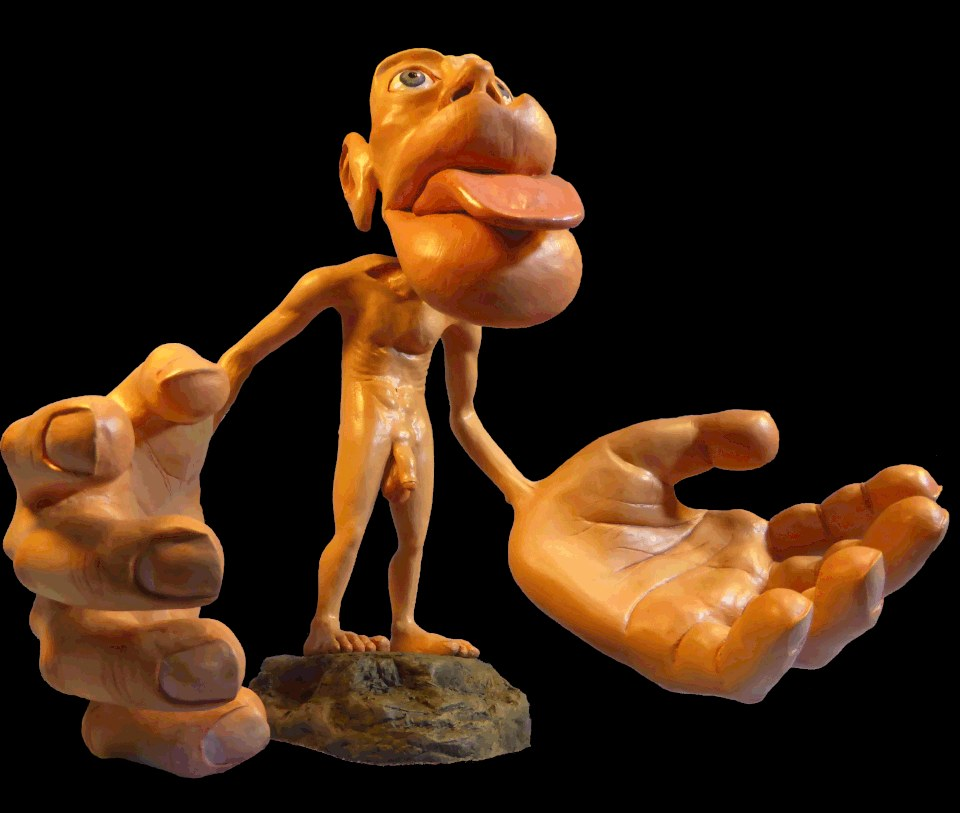
\includegraphics[height=5.0cm]{homunculus_model.jpg}\par
      {\scriptsize Զգացողական հոմունկուլուս (homunculus)}
    \end{column}
    \begin{column}{0.54\textwidth}
      \begin{itemize}
        \item Զգացողական կեղևը մարմնի \textbf{քարտեզ} է. ոտքի հատվածը ոտքի համար, ձեռքինը՝ ձեռքի
        \item<2-> Բայց չափերը \textbf{իրական չեն}. կուրծքն ու մեջքը փոքր տեղ ունեն, ձեռքերն ու շուրթերը՝ հսկայական
        \item<3-> Ներբանները շատ զգայուն չեն. այլապես ամեն քարի վրա ոտք դնելը տանջանք կլիներ
        \item<4-> «Սեռական օրգանները նույնպես զգայուն են, բայց եկեք չխորանանք» (Բըրնեթ)
      \end{itemize}
    \end{column}
  \end{columns}
\end{frame}

\begin{frame}{Երկու կետ, թե՞ մեկ}
  \begin{columns}[T]
    \begin{column}{0.45\textwidth}
      \begin{tryit}
        Երկու գրիչի ծայրերը պահիր \textbf{մոտ 1 սմ} հեռու ու դիպցրու \textbf{մատիդ ծայրին}, հետո՝ \textbf{նախաբազկին}։ Քանի՞ կետ ես զգում։
      \end{tryit}
      \onslide<3->{%
      \begin{card}[colback=butter!40!cream]
        \emoji{hand}\ Դրա համար են \textbf{Բրայլի} տառերը կետերից. մատի ծայրը սովորական տառեր չի «կարդա»։
      \end{card}}
    \end{column}
    \begin{column}{0.51\textwidth}
      \onslide<2->{%
      {\small\blackfont Ամենափոքր հեռավորությունը, որ երկու կետը զգացվում է որպես երկու, մմ}\par\medskip
      % Two-point discrimination: the smallest gap at which two touches feel like two (normal clinical ranges,
% Bickley & Szilagyi, Bates' Guide, 2007). Range bars on a 0-40 mm axis (use inside a frame).
\begin{tikzpicture}[x=0.1cm, y=1cm]
  \draw[plum, line width=0.8pt] (0,-0.35) -- (41,-0.35);
  \foreach \m in {0,10,20,30,40}{
    \draw[plum, line width=0.8pt] (\m,-0.35) -- (\m,-0.47);
    \node[font=\scriptsize, text=plum, below] at (\m,-0.45) {\m};}
  \foreach \y/\t/\a/\b in {2.4/շուրթեր/2/4, 1.65/մատի ծայր/2/8, 0.9/ափ/8/12, 0.15/{մեջք, սրունք}/30/40}{
    \node[font=\small, text=plum, anchor=east] at (-0.8,\y) {\t};
    \fill[amBlue, rounded corners=1mm] (\a,\y-0.2) rectangle (\b,\y+0.2);
    \node[font=\blackfont\scriptsize, text=plum, anchor=west] at (\b+0.6,\y) {\a-\b};}
\end{tikzpicture}
}
    \end{column}
  \end{columns}
  \onslide<2->{\source{Bickley \& Szilagyi, Bates' Guide, 2007}}
\end{frame}

\begin{frame}{Արիստոտելի իլյուզիա}
  \begin{columns}[c]
    \begin{column}{0.5\textwidth}
      \begin{tryit}
        \begin{enumerate}
          \item Խաչիր ցուցամատդ ու միջնամատդ
          \item \textbf{Փակիր աչքերդ}
          \item Խաչված մատների ծայրերով շոշափիր գնդիկը, մետաղադրամի եզրը կամ քթիդ ծայրը
        \end{enumerate}
        Քանի՞ առարկա ես զգում։
      \end{tryit}
    \end{column}
    \begin{column}{0.46\textwidth}
      \centering
      % Aristotle's illusion: with crossed fingers, one small ball touches the two "outer" sides of the
% fingertips, and the brain reports two balls. The thought bubble appears on slide 2 (use inside a frame).
\begin{tikzpicture}[scale=0.82]
  \path[use as bounding box] (-2.0,-2.3) rectangle (3.6,2.5);
  % palm
  \filldraw[fill=peach!70!cardwhite, draw=plum, line width=0.9pt, rounded corners=4mm] (-1.05,-2.25) rectangle (1.05,-1.05);
  % index finger (under), then middle finger (over), crossed
  \draw[plum, line width=0.56cm, line cap=round] (-0.42,-1.15) -- (0.5,1.05);
  \draw[peach!70!cardwhite, line width=0.42cm, line cap=round] (-0.42,-1.15) -- (0.5,1.05);
  \draw[plum, line width=0.56cm, line cap=round] (0.42,-1.15) -- (-0.5,1.05);
  \draw[peach!70!cardwhite, line width=0.42cm, line cap=round] (0.42,-1.15) -- (-0.5,1.05);
  % the ball between the crossed tips
  \shade[ball color=amBlue!70] (0,1.62) circle (0.3);
  \node[font=\blackfont\small, text=plum, anchor=east] at (-0.6,1.75) {1 գնդիկ};
  % what the brain reports
  \node[think, visible on=<2->, callout absolute pointer={(0.7,1.75)}, minimum width=2.4cm, minimum height=1.6cm]
    at (2.45,1.55) {\tikz{\shade[ball color=amBlue!70] (0,0) circle (0.2); \shade[ball color=amBlue!70] (0.55,0) circle (0.2);}\\[1mm] 2 գնդիկ};
\end{tikzpicture}
\par
      \onslide<3->{\raggedright\small Զգացողական կեղևը «չգիտի», որ մատները խաչված են, իսկ փակ աչքերը չեն կարող օգնել։\par}
    \end{column}
  \end{columns}
\end{frame}

\begin{frame}{Գեները կապում են լսողությունն ու հպումը}
  \begin{columns}[c]
    \begin{column}{0.56\textwidth}
      \begin{itemize}
        \item 2012. Ֆրենցելն (Frenzel) ու գործընկերները ցույց տվեցին, որ գեները ազդում են նաև \textbf{հպման զգայունության} վրա
        \item<2-> Ով շատ լավ է լսում, սովորաբար ավելի նուրբ հպում էլ ունի. ով վատ է լսում, հաճախ վատ է զգում նաև հպումը
        \item<3-> Գտան նաև մի մուտացված գեն, որը վնասում է \textbf{երկուսն էլ}
      \end{itemize}
    \end{column}
    \begin{column}{0.4\textwidth}
      \centering
      \bigemoji[1.2cm]{ear}\ {\Large $\leftrightarrow$}\ \bigemoji[1.2cm]{hand}\par\medskip
      \onslide<4->{%
      \begin{card}[colback=mint!35!cardwhite]
        Ուրեմն ռիթմը զգալը, գուցե, ավելի \textbf{բառացի} է, քան կարծում էինք \emoji{musical}
      \end{card}}
    \end{column}
  \end{columns}
  \source{Frenzel et al., PLOS Biology, 2012}
\end{frame}

\begin{frame}{Առաջին կեսը՝ մեկ էջում}
  \begin{columns}[T]
    \begin{column}{0.47\textwidth}
      \begin{card}\emoji{nose}\ {\blackfont Հոտ}\par Թերագնահատված է. 1 տրիլիո՞ն հոտ, ուղիղ կապ հիշողության ու զգացմունքների հետ\end{card}
      \begin{card}\emoji{tongue}\ {\blackfont Համ}\par Ամենաթույլը. մեծ մասը հոտն է, մնացածը՝ ակնկալիքը\end{card}
    \end{column}
    \begin{column}{0.47\textwidth}
      \begin{card}\emoji{ear}\ {\blackfont Լսողություն}\par Մեխանիկական. խխունջը հաճախականությունների քարտեզ է\end{card}
      \begin{card}\emoji{hand}\ {\blackfont Հպում}\par Ուղեղում մարմնի աղավաղված քարտեզ, ու այն էլ է խաբվում\end{card}
    \end{column}
  \end{columns}
  \vspace{1mm}
  \centering\small Ուղեղը սիրում է զգայարանները \textbf{զույգերով} խմբավորել, ավելի հաճախ, քան գործնական է։
\end{frame}

% ---------------------------------------------------------------- break
\begin{frame}[plain]
  \begin{tikzpicture}[remember picture, overlay]
    \fill[butter!60!cream] (current page.south west) rectangle (current page.north east);
    \node at ([yshift=8mm]current page.center) {\mascot[4cm]{sleepy}};
    \node[anchor=north, font=\titlefont\fontsize{30}{32}\selectfont, text=plum] at ([yshift=-17mm]current page.center) {Ընդմիջում};
    \node[anchor=north, font=\mediumfont\large, text=plum] at ([yshift=-31mm]current page.center)
      {5 րոպե \emoji{coffee}\quad Կանգնիր, ձգվիր, ջուր խմիր};
  \end{tikzpicture}
\end{frame}

% ===== Section 3: Jesus has returned ... as a piece of toast? (vision, ~24 min) =====
\topicopener{eye}{Տեսողություն}{Հիսուսը վերադարձել է... տոստի կտորի տեսքո՞վ}{Ինչ չգիտեիր տեսողական համակարգի մասին}{confused}

\begin{frame}{Ի՞նչն է ընդհանուր}
  \begin{columns}[c]
    \begin{column}{0.56\textwidth}
      {\centering
      \bigemoji[0.95cm]{bread}\ \bigemoji[0.95cm]{pizza}\ \bigemoji[0.95cm]{icecream}\ \bigemoji[0.95cm]{banana}\ \bigemoji[0.95cm]{chips}\ \bigemoji[0.95cm]{wood}\par}
      \medskip
      \begin{chatbox}
        Տոստ, տակո, պիցցա, պաղպաղակ, բանան, չիպս, լաքապատ փայտ... Ի՞նչն է ընդհանուր։ Գրիր չաթում։
      \end{chatbox}
      \onslide<2->{%
      \begin{card}[colback=butter!45!cream]
        Բոլորի վրա «տեսել են» \textbf{Հիսուսի դեմքը}։ Երբեմն՝ Մարիամ Աստվածածնի։ Կամ \textbf{Էլվիս Փրեսլիի}։ «Լուրջ, փնտրիր» (Բըրնեթ)։
      \end{card}}
    \end{column}
    \begin{column}{0.4\textwidth}
      \centering
      % A slice of toast whose burnt patches happen to make a face (pareidolia). No reveals.
\begin{tikzpicture}[scale=0.95]
  % crust and bread
  \filldraw[fill=peachdark!75!brown, draw=plum, line width=1pt]
    (-1.55,-1.7) -- (-1.55,0.75) .. controls (-2.05,1.1) and (-1.95,2.05) .. (-0.9,2.1)
    .. controls (-0.3,2.45) and (0.3,2.45) .. (0.9,2.1) .. controls (1.95,2.05) and (2.05,1.1) .. (1.55,0.75)
    -- (1.55,-1.7) -- cycle;
  \fill[butter!80!peach]
    (-1.35,-1.5) -- (-1.35,0.8) .. controls (-1.75,1.1) and (-1.7,1.85) .. (-0.85,1.88)
    .. controls (-0.3,2.2) and (0.3,2.2) .. (0.85,1.88) .. controls (1.7,1.85) and (1.75,1.1) .. (1.35,0.8)
    -- (1.35,-1.5) -- cycle;
  % toasted shading
  \fill[peachdark, opacity=0.18] (0,0.3) ellipse (1.2 and 1.5);
  % burnt patches: eyes, nose, mouth, beard
  \fill[plum!80!brown, opacity=0.55] (-0.55,0.95) ellipse (0.28 and 0.17);
  \fill[plum!80!brown, opacity=0.55] (0.55,0.95) ellipse (0.28 and 0.17);
  \fill[plum!80!brown, opacity=0.35] (-0.05,0.55) .. controls (-0.2,0.2) and (-0.15,0.0) .. (0.15,0.02) -- (0.1,0.2) -- cycle;
  \fill[plum!80!brown, opacity=0.45] (-0.5,-0.35) .. controls (-0.2,-0.55) and (0.2,-0.55) .. (0.5,-0.35)
    .. controls (0.2,-0.42) and (-0.2,-0.42) .. cycle;
  \fill[plum!80!brown, opacity=0.2] (-0.9,-0.1) .. controls (-0.8,-1.2) and (0.8,-1.2) .. (0.9,-0.1)
    .. controls (0.6,-0.85) and (-0.6,-0.85) .. cycle;
  % crumbs
  \foreach \x/\y in {-1.0/-1.1, 0.9/-0.9, 1.0/1.5, -1.1/1.55, 0.3/-1.25}{\fill[peachdark!70] (\x,\y) circle (0.04);}
\end{tikzpicture}

    \end{column}
  \end{columns}
\end{frame}

\begin{frame}{Դեմքեր ամենուր}
  \begin{columns}[c]
    \begin{column}{0.5\textwidth}
      \centering
      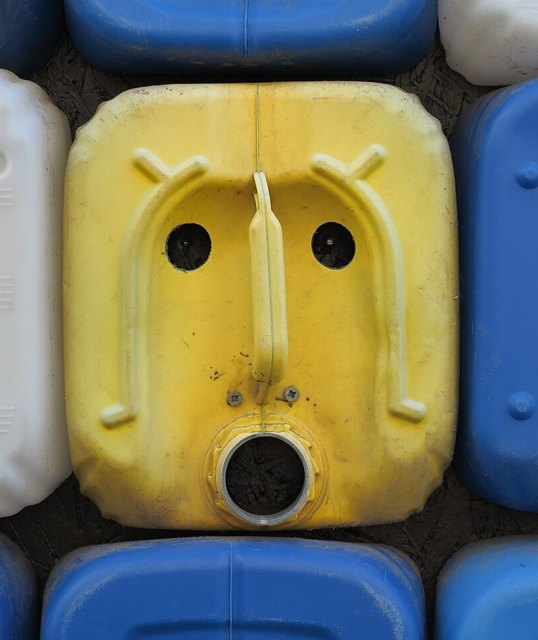
\includegraphics[height=2.45cm]{pareidolia_canister.jpg}\hspace{1mm}%
      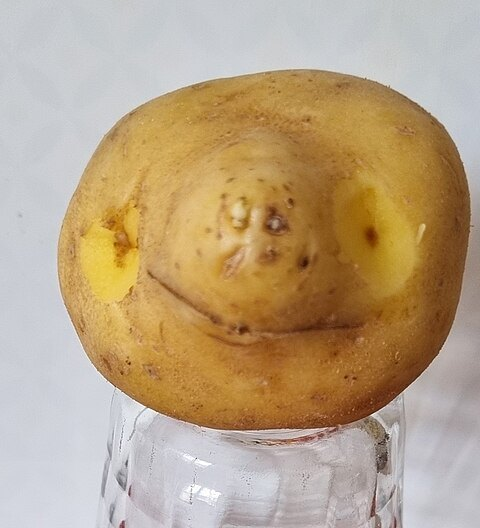
\includegraphics[height=2.45cm]{pareidolia_potato.jpg}\par\vspace{1mm}
      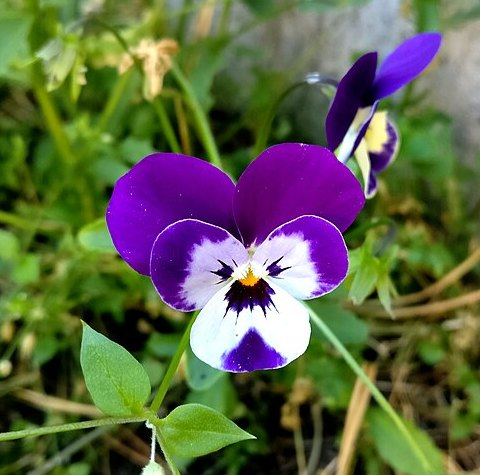
\includegraphics[height=2.45cm]{pareidolia_pansy.jpg}\hspace{1mm}%
      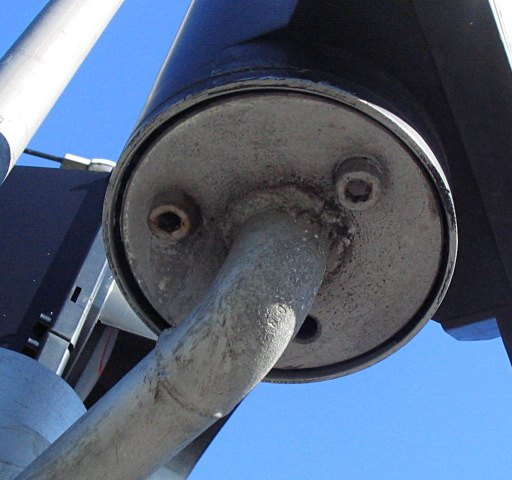
\includegraphics[height=2.45cm]{pareidolia_lamp.jpg}
    \end{column}
    \begin{column}{0.46\textwidth}
      \begin{itemize}
        \item Աշխարհում միլիարդավոր առարկաներ ունեն լուսավոր ու մուգ պատահական բծեր
        \item<2-> Պատահաբար որոշները նման են \textbf{դեմքի}։ Դա կոչվում է \textbf{պարեյդոլիա} (pareidolia)
        \item<3-> Տարօրինակն այն է, որ նույնիսկ գիտենալով, որ սա կարտոֆիլ է, դեմքը \textbf{չես կարող չտեսնել}
      \end{itemize}
    \end{column}
  \end{columns}
\end{frame}

\begin{frame}{Դեմք Մարսի վրա}
  \begin{columns}[T]
    \begin{column}{0.4\textwidth}
      \centering
      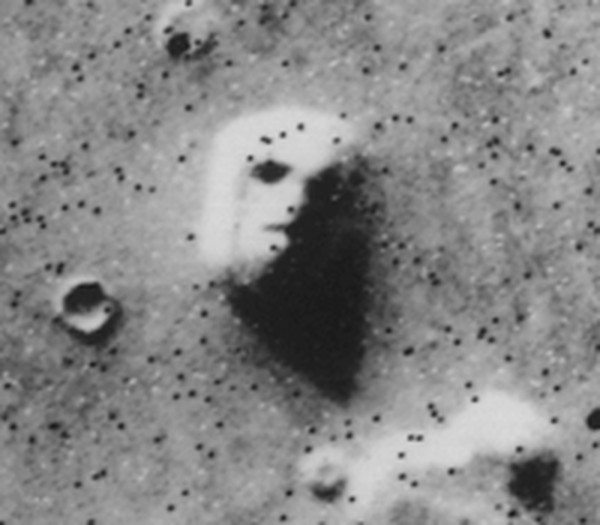
\includegraphics[height=4.1cm]{mars_face_viking_1976.jpg}\par
      {\scriptsize «Վիկինգ 1», 1976}
    \end{column}
    \begin{column}{0.56\textwidth}
      \onslide<2->{%
      \begin{columns}[T]
        \begin{column}{0.48\linewidth}
          \centering
          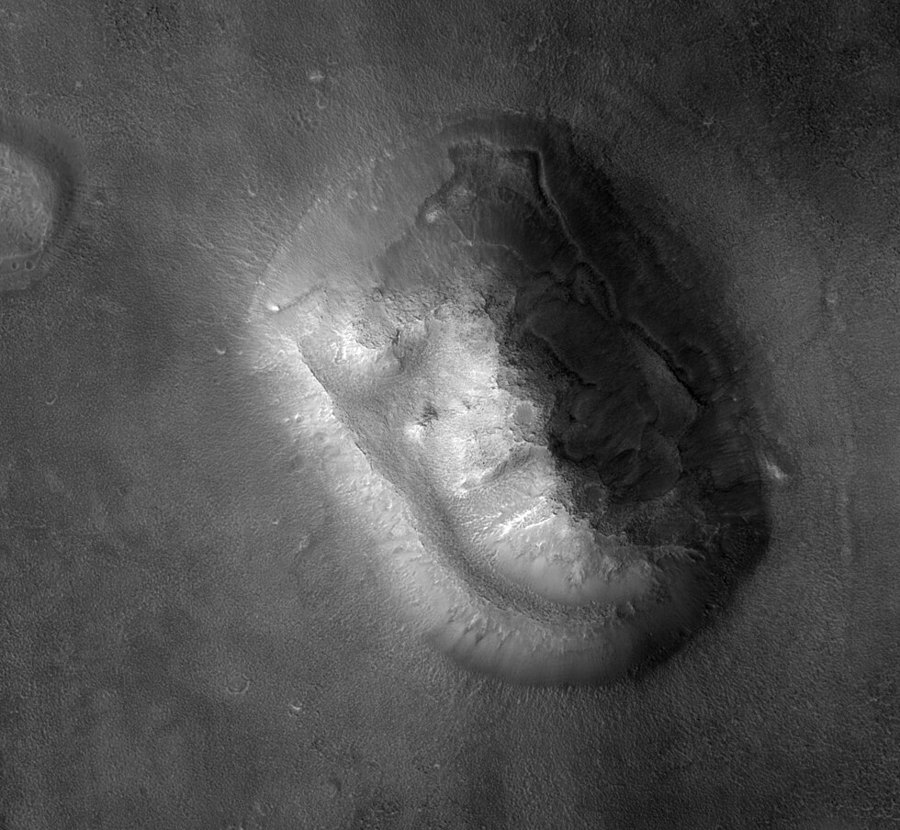
\includegraphics[height=2.9cm]{mars_face_hirise_2007.jpg}\par
          {\scriptsize Նույն բլուրը, 2007}
        \end{column}
        \begin{column}{0.5\linewidth}
          \small 1976-ին ՆԱՍԱ-ի նկարում Մարսի վրա «դեմք» երևաց։ Ավելի լավ տեսախցիկը ցույց տվեց սովորական \textbf{բլուր}։
        \end{column}
      \end{columns}}
      \vspace{2mm}
      \onslide<3->{%
      \begin{card}[colback=lavender!40!cardwhite]
        \small Ձախ նկարում դեմքը հիմա էլ տեսնում ես։ Ուղեղը դեմքեր փնտրում է \textbf{ամենուր}։
      \end{card}}
    \end{column}
  \end{columns}
  \source{NASA/JPL (Viking 1; MRO HiRISE)}
\end{frame}

\begin{frame}{Աչքերը տեսախցիկ չեն}
  \begin{columns}[T]
    \begin{column}{0.5\textwidth}
      \begin{itemize}
        \item Ուղեղը տեսողությունը գերադասում է \textbf{բոլոր} մյուս զգայարաններից
        \item<2-> Բայց աչքերը «երկու անհանգստացնող փափուկ տեսախցիկ» չեն, որոնք ամեն ինչ ուղիղ ուղեղ են փոխանցում
        \item<3-> Շատ նեյրոգիտնականներ \textbf{ցանցաթաղանթը} (retina) համարում են ուղեղի մաս. նույն հյուսվածքից է զարգանում ու ուղիղ կապված է նրան
      \end{itemize}
    \end{column}
    \begin{column}{0.46\textwidth}
      \onslide<4->{%
      \begin{bookquote}
        Աչքը այնքան բարդ է, որ այն բերում են որպես ապացույց, թե էվոլյուցիան իրական չէ։ Բայց եթե նայես, թե ինչպես է աչքը աշխատում, ստեղծողը այն նախագծել է ուրբաթ կեսօրից հետո կամ խումհարով։
      \end{bookquote}}
    \end{column}
  \end{columns}
\end{frame}

\begin{frame}{Ցուպիկներ ու սրվակներ}
  \begin{columns}[T]
    \begin{column}{0.47\textwidth}
      \begin{card}[colback=lavender!35!cardwhite]
        \tikz[baseline=-0.5ex]{\filldraw[fill=night!70, draw=plum, line width=0.6pt, rounded corners=0.6mm] (0,-0.12) rectangle (0.9,0.12);}\
        {\blackfont Ցուպիկներ} (rods)\par\smallskip
        \begin{itemize}
          \item Արձագանքում են ընդամենը \textbf{մոտ 6 ֆոտոնի}
          \item Լույս ու մութ, կոնտրաստ. աշխատում են \textbf{մթնշաղին}
          \item Ցերեկը «խեղդվում» են. մի դույլ ջուր՝ ձվի բաժակի մեջ
        \end{itemize}
      \end{card}
    \end{column}
    \begin{column}{0.47\textwidth}
      \onslide<2->{%
      \begin{card}[colback=peach!40!cardwhite]
        \tikz[baseline=-0.5ex]{\filldraw[fill=amOrange, draw=plum, line width=0.6pt] (0,-0.14) -- (0.75,-0.05) -- (0.75,0.05) -- (0,0.14) -- cycle;}\
        {\blackfont Սրվակներ} (cones)\par\smallskip
        \begin{itemize}
          \item Զգում են լույսի ալիքի երկարությունը՝ \textbf{գույնը}
          \item Ավելի մանրամասն պատկեր են տալիս
          \item Շատ լույս է պետք. դրա համար մթնշաղին գույներ չենք տեսնում
        \end{itemize}
      \end{card}}
    \end{column}
  \end{columns}
  \vspace{2mm}
  \onslide<3->{\centering\small\emoji{siren}\ Ցուպիկների զգայունությունը, ըստ Բըրնեթի, բանկի ահազանգ է, որ միանում է, երբ ինչ-որ մեկը \textbf{միայն մտածում է} կողոպուտի մասին։\par}
\end{frame}

\begin{frame}{Աչքի ներսում}
  \begin{columns}[c]
    \begin{column}{0.54\textwidth}
      \centering
      % Cross-section of the eye (light comes from the left): pupil, lens, retina, fovea, optic nerve.
% The fovea is highlighted on slide 2 (use inside a frame).
\begin{tikzpicture}[
    tagl/.style={font=\scriptsize, text=plum, align=center, inner sep=1.5pt},
  ]
  \path[use as bounding box] (-4.2,-2.25) rectangle (3.6,2.2);
  % optic nerve (behind the eyeball)
  \filldraw[fill=butter!80!cardwhite, draw=plum, line width=0.9pt]
    (1.35,-0.45) .. controls (2.2,-0.5) and (2.8,-0.75) .. (3.6,-0.95) -- (3.6,-0.25)
    .. controls (2.8,-0.05) and (2.2,0.05) .. (1.45,0.0) -- cycle;
  % eyeball and cornea
  \filldraw[fill=cardwhite, draw=plum, line width=1.1pt] (0,0) circle (1.6);
  \draw[plum, line width=1.1pt, fill=lavender!30!cardwhite] (-1.38,0.8) .. controls (-1.95,0.45) and (-1.95,-0.45) .. (-1.38,-0.8);
  % retina lining the back
  \draw[brainpink!90!plum, line width=3.2pt] (115:1.47) arc (115:-115:1.47);
  % iris with the pupil gap, lens
  \draw[amBlue!70, line width=3pt] (-1.42,0.78) -- (-1.42,0.28) (-1.42,-0.28) -- (-1.42,-0.78);
  \filldraw[fill=lavender!60!cardwhite, draw=plum, line width=0.8pt] (-1.05,0) ellipse (0.2 and 0.58);
  % light from an object, focused on the fovea
  \node at (-3.75,0.95) {\bigemoji[0.7cm]{tree}};
  \draw[amOrange, line width=0.9pt] (-3.45,0.95) -- (-1.05,0.45) -- (1.47,0.0);
  \draw[amOrange, line width=0.9pt] (-3.45,0.95) -- (-1.05,-0.4) -- (1.47,0.0);
  % fovea
  \fill[amRed] (1.47,0.0) circle (0.09);
  \begin{scope}[visible on=<2->]
    \draw[amRed, line width=1.4pt] (1.47,0) circle (0.24);
  \end{scope}
  % labels
  \node[tagl, anchor=south] at (-1.42,1.0) {բիբ};
  \draw[plum!70, line width=0.5pt] (-1.42,1.02) -- (-1.42,0.4);
  \node[tagl, anchor=north] at (-1.05,-0.95) {ոսպնյակ};
  \draw[plum!70, line width=0.5pt] (-1.05,-0.95) -- (-1.05,-0.6);
  \node[tagl, anchor=south west] at (0.75,1.6) {\textbf{ցանցաթաղանթ} (retina)};
  \draw[plum!70, line width=0.5pt] (0.95,1.62) -- (0.78,1.25);
  \node[tagl, anchor=west, font=\blackfont\scriptsize, text=amRed] at (1.95,0.55) {ֆովեա (fovea)};
  \draw[amRed, line width=0.6pt] (1.97,0.55) -- (1.6,0.12);
  \node[tagl, anchor=north] at (2.75,-1.05) {տեսողական նյարդ};
\end{tikzpicture}

    \end{column}
    \begin{column}{0.42\textwidth}
      \begin{itemize}
        \item Լույսը մտնում է բբով ու ոսպնյակով ու ընկնում ցանցաթաղանթի վրա
        \item<2-> Ֆոտոընկալիչները միանում են այլ բջիջների, որոնք տեղեկությունը տանում են ուղեղ
        \item<3-> Մի խումբ ընկալիչ, որ «խոսում է» նույն բջջի հետ, կոչվում է \textbf{ընկալող դաշտ} (receptive field). ինչպես հեռախոսները մեկ աշտարակի տարածքում
      \end{itemize}
    \end{column}
  \end{columns}
\end{frame}

\begin{frame}{Ընկալող դաշտեր}
  \centering
  % Receptive fields along the retina: in the periphery many photoreceptors share one ganglion cell
% (a big field, like a golf umbrella), in the centre one or two do (small, sharp fields). Reveals 1-2.
\begin{tikzpicture}[x=1cm, y=1cm]
  \path[use as bounding box] (-6.5,-1.75) rectangle (6.5,0.95);
  % photoreceptors
  \foreach \i in {-24,...,24}{\fill[plum] (\i*0.25,0) circle (0.06);}
  % fields: start/end x of each group
  \foreach \a/\b/\c in {-6.0/-4.5/lavender, -4.25/-2.75/lavender, -2.5/-1.5/lavender!60!brainpink,
      -1.25/-0.75/brainpink, -0.5/-0.25/brainpink, 0/0/pinkdark!60, 0.25/0.5/brainpink, 0.75/1.25/brainpink,
      1.5/2.5/lavender!60!brainpink, 2.75/4.25/lavender, 4.5/6.0/lavender}{
    \draw[\c, line width=1.2pt, rounded corners=1.5mm] (\a-0.12,-0.17) rectangle (\b+0.12,0.17);
    \draw[plum!60, line width=0.6pt] ({(\a+\b)/2},-0.17) -- ({(\a+\b)/2},-0.75);
    \filldraw[fill=\c, draw=plum, line width=0.6pt] ({(\a+\b)/2},-0.85) circle (0.1);}
  \node[font=\scriptsize, text=plum, anchor=west] at (-6.5,-1.2) {ամեն շրջանակը մեկ «աշտարակ» է (ganglion cell)};
  % labels
  \node[font=\blackfont\scriptsize, text=plum] at (-4.6,0.6) {ծայրամաս՝ մեծ դաշտեր};
  \node[font=\blackfont\scriptsize, text=pinkdark] at (0,0.6) {կենտրոն՝ փոքր դաշտեր};
  \node[font=\blackfont\scriptsize, text=plum] at (4.6,0.6) {ծայրամաս՝ մեծ դաշտեր};
  \node[visible on=<2->, font=\scriptsize, text=plum, align=center] at (4.2,-1.4)
    {\emoji{star}\ մեծ դաշտ = անձրևանոց. գիտես, որ կաթիլ ընկավ,\\ բայց չգիտես՝ ճիշտ որտեղ};
\end{tikzpicture}
\par\medskip
  \begin{columns}[T]
    \begin{column}{0.47\textwidth}
      \begin{card}[colback=lavender!35!cardwhite]
        \small Ծայրամասում դաշտերը \textbf{մեծ} են, ինչպես գոլֆի անձրևանոց. ճշգրտությունը տուժում է։
      \end{card}
    \end{column}
    \begin{column}{0.47\textwidth}
      \onslide<2->{%
      \begin{card}[colback=brainpink!30!cardwhite]
        \small Կենտրոնում դաշտերը \textbf{փոքր ու խիտ} են, ու տեսնում ենք մանր տառերը։
      \end{card}}
    \end{column}
  \end{columns}
\end{frame}

\begin{frame}{Ֆովեա՝ մատնահետք հեռուստացույցի վրա}
  \begin{columns}[c]
    \begin{column}{0.5\textwidth}
      \centering
      % Burnett's comparison: if the retina were a widescreen TV, the fovea would be a thumbprint in the
% middle. Everything outside it is blurry outlines. The thumbprint appears on slide 2.
\begin{tikzpicture}
  \path[use as bounding box] (-3.6,-2.35) rectangle (3.6,2.2);
  % the TV
  \filldraw[fill=plum, draw=plum, rounded corners=2mm] (-3.45,-1.85) rectangle (3.45,2.05);
  \fill[night!80!lavender] (-3.25,-1.65) rectangle (3.25,1.85);
  \draw[plum, line width=2pt] (-0.6,-1.85) -- (-0.9,-2.3) (0.6,-1.85) -- (0.9,-2.3);
  % blurry outlines of a scene
  \fill[mint, opacity=0.25] (-3.25,-1.65) rectangle (3.25,-0.6);
  \fill[butter, opacity=0.3] (2.2,1.2) circle (0.5);
  \fill[peach, opacity=0.25] (-2.4,-0.7) rectangle (-1.4,0.5);
  \fill[lavender, opacity=0.25] (1.0,-0.7) rectangle (2.3,0.9);
  \fill[brainpink, opacity=0.25] (-2.0,0.95) ellipse (0.6 and 0.25);
  % the thumbprint: the only sharp part
  \begin{scope}[visible on=<2->]
    \fill[cardwhite] (0,0.1) ellipse (0.3 and 0.38);
    \foreach \r in {0.06,0.12,0.18,0.24}{\draw[plum, line width=0.45pt] (0,0.1) ellipse ({\r} and {\r*1.3});}
    \draw[amOrange, line width=1.2pt] (0,0.1) ellipse (0.36 and 0.45);
    \draw[amOrange, line width=0.8pt] (0.36,0.25) -- (1.6,1.35) node[anchor=south, font=\blackfont\scriptsize, text=butter, fill=plum, inner sep=2pt] {ֆովեա};
  \end{scope}
\end{tikzpicture}

    \end{column}
    \begin{column}{0.46\textwidth}
      \begin{itemize}
        \item Մանրամասները տեսնում է միայն \textbf{ֆովեան}՝ ցանցաթաղանթի \textbf{1\%-ից էլ քիչ} մասը
        \item<2-> Եթե ցանցաթաղանթը լայնէկրան հեռուստացույց լիներ, ֆովեան մեջտեղի մատնահետքը կլիներ
        \item<3-> Մնացածը մշուշոտ ուրվագծեր են. ասես նայում ես վազելինից պատրաստված հեռադիտակի սխալ ծայրից
      \end{itemize}
    \end{column}
  \end{columns}
\end{frame}

\begin{frame}{Փորձիր հիմա. մի շարժիր աչքերդ}
  \begin{tryit}
    Նայիր \textbf{կարմիր կետին} ու աչքերդ մի շարժիր։ Կարո՞ղ ես կարդալ կողքի բառերը։
  \end{tryit}
  \vspace{2mm}
  % Fovea demo: fixate the dot and try to read the words without moving the eyes.
\begin{tikzpicture}
  \path[use as bounding box] (-7.0,-0.75) rectangle (7.0,0.75);
  \fill[amRed] (0,0) circle (0.12);
  \draw[amRed, line width=0.8pt] (0,0) circle (0.25);
  \foreach \x/\w in {-6.1/վարդ, -3.9/կոնֆետ, -1.7/ականջ, 1.7/գրիչ, 3.9/աղավնի, 6.1/հացիկ}{
    \node[font=\mediumfont\large, text=plum] at (\x,0) {\w};}
\end{tikzpicture}
\par
  \vspace{2mm}
  \onslide<2->{%
  \begin{card}[width=0.9\textwidth, colback=butter!40!cream]
    \centering Բառերը գիտես, որ կան, բայց կարդալ դժվար է։ Ֆովեայից դուրս ուղեղն ստանում է միայն ուրվագծեր, ու մնացածը \textbf{լրացնում է ինքը}։
  \end{card}}
\end{frame}

\begin{frame}{Լուսարձակ ֆուտբոլի դաշտում}
  \begin{columns}[T]
    \begin{column}{0.5\textwidth}
      \begin{itemize}
        \item Աչքերը անընդհատ շարժվում են, որ ֆովեան ուղղեն կարևոր կետերին
        \item<2-> Ինչպես լուսարձակ ֆուտբոլի դաշտում, որը կառավարում է կոֆեինի \textbf{գրեթե մահացու} չափաբաժին ընդունած մեկը
        \item<3-> Ուղեղը այս կտորներից ու մշուշոտ ֆոնից «հղկում» է պատկերը ու շատ բան \textbf{գուշակում} է
      \end{itemize}
    \end{column}
    \begin{column}{0.46\textwidth}
      \onslide<4->{%
      \begin{card}[colback=peach!40!cardwhite]
        \emoji[1.3em]{basketball}\ Ինչու՞ ֆովեան մեծ չէ։ Այն կրկնապատկելու համար ուղեղը պետք է մեծանար մինչև \textbf{բասկետբոլի գնդակի} չափ։
      \end{card}}
      \onslide<5->{%
      \begin{card}[colback=lavender!35!cardwhite]
        \small\emoji{eyes}\ Աչքի շարժումներին ժամանակին հետևում էին \textbf{մետաղե կոնտակտային ոսպնյակներով}։
      \end{card}}
    \end{column}
  \end{columns}
\end{frame}

\begin{frame}{Ուղին աչքից ուղեղ}
  \begin{columns}[c]
    \begin{column}{0.58\textwidth}
      \centering
      % The visual pathway as in the book: eye -> optic nerve -> thalamus -> visual cortex (occipital lobe);
% side branches to the brainstem: pretectum (pupil size) and superior colliculus (saccades). Reveals 1-3.
\begin{tikzpicture}[
    tag/.style={draw=plum, line width=0.7pt, fill=cardwhite, rounded corners=2mm, inner sep=2.2pt,
      font=\scriptsize, text=plum, align=center},
  ]
  \path[use as bounding box] (-4.1,-2.0) rectangle (4.0,2.0);
  \begin{scope}[scale=0.6]
    \brainlobes{lavender!40!cream}{mint!40!cream}{peach!45!cream}{butter!80!cream}
    % eye in front of the brain
    \filldraw[fill=cardwhite, draw=plum, line width=0.9pt] (-4.2,-0.75) circle (0.45);
    \fill[amBlue!70] (-4.55,-0.75) circle (0.16);
    % thalamus deep inside
    \filldraw[fill=brainpink, draw=plum, line width=0.7pt, dashed] (0.5,0.35) ellipse (0.55 and 0.32);
    % main route
    \draw[amRed, line width=2pt, -{Stealth[length=3mm]}] (-3.75,-0.7) .. controls (-2.0,-0.5) .. (-0.05,0.3);
    \draw[amRed, line width=2pt, -{Stealth[length=3mm]}, visible on=<2->] (1.05,0.35) .. controls (2.0,0.3) .. (2.85,-0.05);
    \fill[amRed, opacity=0.55, visible on=<2->] (3.0,-0.15) ellipse (0.3 and 0.55);
    % brainstem branch
    \draw[amBlue, line width=1.6pt, dashed, -{Stealth[length=2.6mm]}, visible on=<3->] (0.3,0.05) .. controls (0.8,-0.5) .. (1.3,-1.15);
    \fill[amBlue, visible on=<3->] (1.35,-1.25) circle (0.12);
    % labels
    \node[tag] at (-4.5,0.6) {\emoji[1em]{eye}\ աչք};
    \node[tag] (th) at (-1.4,2.75) {\textbf{թալամուս}\\ «գլխավոր կայարան»};
    \draw[plum, line width=0.7pt] (th.south) -- (0.4,0.6);
    \node[tag, visible on=<2->] (vc) at (4.6,1.95) {\textbf{տեսողական կեղև}\\ ծոծրակային բիլթ};
    \draw[plum, line width=0.7pt, visible on=<2->] (vc.south) -- (3.1,0.35);
    \node[tag, visible on=<3->] (bs) at (-1.6,-2.95) {\textbf{ուղեղաբուն}. բբի չափը\\ ու աչքի ցատկերը (saccades)};
    \draw[plum, line width=0.7pt, visible on=<3->] (bs.east) -- (1.2,-1.35);
  \end{scope}
\end{tikzpicture}

    \end{column}
    \begin{column}{0.38\textwidth}
      \begin{itemize}
        \item Տեսողական նյարդերով ազդանշանը գնում է \textbf{թալամուս} {\small(հիշո՞ւմ ես վախի «կայարանը» վեբինար 1-ից)}
        \item<2-> Այնտեղից՝ ուղեղի \textbf{ետևի} մասը
        \item<3-> Մի մասն էլ ուղեղաբուն է գնում. բբի չափն ու աչքի արագ ցատկերը
      \end{itemize}
    \end{column}
  \end{columns}
\end{frame}

\begin{frame}{Առասպել, թե՞ փաստ}
  \mythorfact{Վիրահատության ժամանակ աչքը հանում ու կախ են թողնում նյարդից}{ԱՌԱՍՊԵԼ}{pinkdark}{%
    \begin{card}[width=0.9\textwidth, colback=brainpink!25!cardwhite]
      Նյարդը այնքան չի ձգվում, իսկ աչքը դուրս հանելը կքանդեր այն։ Իրականում կոպերը հետ են քաշում ու աչքը սեղմակներով պահում. դրա համար է տարօրինակ զգացվում։
    \end{card}}
\end{frame}

\begin{frame}{Փորձիր հիմա. ինչպես են շարժվում աչքերդ}
  \begin{columns}[T]
    \begin{column}{0.47\textwidth}
      \begin{tryit}
        \textbf{1.} Դանդաղ տար հայացքդ սենյակի ձախ պատից աջ պատ։ Աչքերդ սահո՞ւն են շարժվում։\par\smallskip
        \onslide<2->{\textbf{2.} Հիմա մատդ դանդաղ տար ձախից աջ ու \textbf{հետևիր} նրան։}
      \end{tryit}
    \end{column}
    \begin{column}{0.49\textwidth}
      \onslide<3->{%
      \begin{card}[colback=lavender!35!cardwhite]
        \textbf{1.} Աչքերը \textbf{ցատկում} են (saccades), ու ուղեղը առանձին «լուսանկարներից» ֆիլմ է սարքում։\par\smallskip
        \textbf{2.} Շարժվող բանի հետևում աչքը \textbf{սահուն} է շարժվում. որսի կամ վտանգի դեպքում պետք է անընդհատ տեսնել։
      \end{card}}
    \end{column}
  \end{columns}
\end{frame}

\begin{frame}{Ցատկեր ու սահուն հետևում}
  \centering
  % Eye position over time: looking across a room = jumps (saccades), following a moving finger = smooth
% (pursuit). The second panel appears on slide 2 (use inside a frame).
\begin{tikzpicture}[
    ax/.style={-{Stealth[length=2mm]}, plum, line width=0.8pt},
    axl/.style={font=\scriptsize, text=plum},
  ]
  % saccades
  \draw[ax] (0,0) -- (4.4,0) node[axl, below left] {ժամանակ};
  \draw[ax] (0,0) -- (0,2.3) node[axl, above right, align=left] {աչքի դիրքը};
  \draw[amRed, line width=1.6pt, line join=round]
    (0.1,0.2) -- (0.8,0.2) -- (0.86,0.75) -- (1.6,0.75) -- (1.66,1.15) -- (2.4,1.15) -- (2.46,1.7) -- (3.3,1.7) -- (3.36,2.0) -- (4.1,2.0);
  \node[font=\blackfont\small, text=plum] at (2.1,-0.5) {նայում ես սենյակով մեկ};
  \node[font=\scriptsize, text=amRed] at (2.1,-0.9) {ցատկեր (saccades)};
  % smooth pursuit
  \begin{scope}[xshift=5.6cm, visible on=<2->]
    \draw[ax] (0,0) -- (4.4,0) node[axl, below left] {ժամանակ};
    \draw[ax] (0,0) -- (0,2.3);
    \draw[amBlue, line width=1.6pt] (0.1,0.2) .. controls (1.5,0.5) and (2.8,1.6) .. (4.1,2.0);
    \node[font=\blackfont\small, text=plum] at (2.1,-0.5) {հետևում ես մատիդ};
    \node[font=\scriptsize, text=amBlue] at (2.1,-0.9) {սահուն հետևում (pursuit)};
  \end{scope}
\end{tikzpicture}
\par
  \begin{columns}[T]
    \begin{column}{0.47\textwidth}
      \onslide<3->{\small Ցատկերի միջև գրեթե ոչինչ չենք տեսնում, ինչպես անիմացիայի կադրերի միջև։ Սակադը մարմնի \textbf{ամենաարագ} շարժումներից է՝ թարթելու ու մայրիկի ներս մտնելիս նոութբուքը փակելու հետ։}
    \end{column}
    \begin{column}{0.47\textwidth}
      \onslide<4->{\small Երբ շարժվող բանը դուրս է գալիս տեսադաշտից, աչքերը ցատկով ետ են գալիս (optokinetic reflex)։ Ուղեղը կարող է աչքերը սահուն շարժել, բայց հաճախ \textbf{չի անում}։}
    \end{column}
  \end{columns}
\end{frame}

\begin{frame}{Ինչու աշխարհը չի ցատկում}
  \begin{columns}[T]
    \begin{column}{0.52\textwidth}
      \begin{itemize}
        \item Երբ աչքերդ շարժվում են, ցանցաթաղանթի պատկերն էլ է շարժվում։ Ինչու՞ է աշխարհը անշարժ թվում
        \item<2-> Աչքի մկանները ազդանշան են ստանում \textbf{ներքին ականջի} հավասարակշռության համակարգից {\small(վեբինար 1-ի ծովախտը)}
        \item<3-> Այդպես ուղեղը տարբերում է «ես եմ շարժվում»-ը «աշխարհն է շարժվում»-ից
      \end{itemize}
    \end{column}
    \begin{column}{0.44\textwidth}
      \onslide<4->{%
      \begin{card}[colback=peach!40!cardwhite]
        \emoji[1.3em]{stethoscope}\ Երբ այս համակարգը սխալ ազդանշան է տալիս, աչքերն ինքնաբերաբար ցնցվում են. \textbf{նիստագմ} (nystagmus)։\par\smallskip
        Բժշկի համար սա նույնն է, ինչ մեխանիկի համար շարժիչի տարօրինակ ձայնը։
      \end{card}}
    \end{column}
  \end{columns}
\end{frame}

\begin{frame}{Եզրեր. ինչպես ենք տեսնում առարկաները}
  \centering
  % Orientation selectivity in the primary visual cortex (Hubel & Wiesel): one neuron fires a lot for a
% bar at its preferred angle (here vertical) and little for others. Panels appear on slides 1-4.
\begin{tikzpicture}[scale=0.78]
  \path[use as bounding box] (-1.1,-2.15) rectangle (10.3,1.1);
  \foreach \i/\a/\n/\s in {0/90/14/1, 1/45/4/2, 2/0/1/3, 3/135/4/4}{
    \begin{scope}[xshift=\i*3.05cm, visible on=<\s->]
      % receptive field with a bar
      \filldraw[fill=cardwhite, draw=plum, line width=0.8pt] (0.9,0.1) circle (0.95);
      \fill[amOrange, rotate around={\a:(0.9,0.1)}] (0.25,0.0) rectangle (1.55,0.2);
      % spike train
      \draw[plum!40, line width=0.6pt] (-0.1,-1.45) -- (1.9,-1.45);
      \pgfmathsetmacro{\spikestep}{1.9/(\n+1)}
      \foreach \k in {1,...,\n}{\draw[amRed, line width=1.2pt] ({-0.1+\k*\spikestep},-1.45) -- ({-0.1+\k*\spikestep},-0.95);}
      \node[font=\blackfont\scriptsize, text=plum] at (0.9,-1.85) {\n\ ազդանշան};
    \end{scope}}
  \node[font=\scriptsize, text=plum, anchor=east, align=right] at (-0.2,-1.2) {նեյրոնը};
\end{tikzpicture}
\par\smallskip
  \begin{columns}[T]
    \begin{column}{0.54\textwidth}
      \onslide<5->{\small Առաջնային տեսողական կեղևը \textbf{սյուներ} է, ինչպես կտրատած հացը։ Ամեն սյուն սիրում է \textbf{մեկ ուղղության} գիծ։ Այդպես ենք տեսնում եզրերը, ուրեմն՝ առարկաներն ու նրանց շարժումը։}
    \end{column}
    \begin{column}{0.42\textwidth}
      \onslide<6->{%
      \begin{scienceupdate}
        Հյուբելն ու Վիզելը սա գտան 1959-1962-ին։ 1981-ը, որ նշված է գրքում, Նոբելյան մրցանակի տարին է։
      \end{scienceupdate}}
    \end{column}
  \end{columns}
  \onslide<6->{\source{Nobel Prize in Physiology or Medicine 1981}}
\end{frame}

\begin{frame}{Գույնի հաստատունություն}
  \begin{columns}[c]
    \begin{column}{0.5\textwidth}
      \centering
      \begin{tikzpicture}
        \fill[butter!60!cardwhite, rounded corners=2mm] (-2.9,-1.3) rectangle (-0.15,1.3);
        \fill[night!70, rounded corners=2mm] (0.15,-1.3) rectangle (2.9,1.3);
        \node at (-2.4,0.85) {\bigemoji[0.6cm]{sun}};
        \node at (2.4,0.85) {\bigemoji[0.6cm]{moon}};
        \fill[amRed] (-1.5,-0.2) circle (0.6);
        \fill[amRed!45!black] (1.5,-0.2) circle (0.6);
        \node[font=\scriptsize, text=plum] at (-1.5,-1.05) {պայծառ լույս};
        \node[font=\scriptsize, text=cardwhite] at (1.5,-1.05) {աղոտ լույս};
        \node[visible on=<2->, draw=plum, line width=0.8pt, fill=cardwhite, rounded corners=2mm, font=\blackfont\small,
              text=plum] at (0,-1.75) {ուղեղ՝ «երկուսն էլ կարմիր են»};
      \end{tikzpicture}
    \end{column}
    \begin{column}{0.46\textwidth}
      \begin{itemize}
        \item Ցանցաթաղանթի համար սրանք \textbf{տարբեր} գույներ են
        \item<2-> Երկրորդային տեսողական կեղևը հաշվի է առնում լույսը ու որոշում, թե ինչ գույն «պետք է» լինի առարկան
        \item<3-> Բայց ոչ 100\%-ով. եթե վիճել ես, թե մեքենան մուգ կապույտ է, թե սև, տեսել ես, թե ինչպես է այն \textbf{շփոթվում}
      \end{itemize}
    \end{column}
  \end{columns}
\end{frame}

\begin{frame}{Նույն գույնը, տարբեր ֆոն}
  \centering
  % Simultaneous contrast: one uniform grey bar on a dark-to-light background looks lighter on the left
% and darker on the right. Slide 2 swaps the background for a plain one (use inside a frame).
\begin{tikzpicture}
  \path[use as bounding box] (-5.0,-1.5) rectangle (5.0,1.5);
  \shade[left color=black!92, right color=white] (-5.0,-1.4) rectangle (5.0,1.4);
  \fill[cardwhite, visible on=<2->] (-5.0,-1.4) rectangle (5.0,1.4);
  \draw[plum, line width=0.8pt] (-5.0,-1.4) rectangle (5.0,1.4);
  \fill[black!50] (-4.3,-0.28) rectangle (4.3,0.28);
\end{tikzpicture}
\par\medskip
  \begin{columns}[T]
    \begin{column}{0.47\textwidth}
      \small Մոխրագույն շերտը ձախում ավելի բաց է թվում, աջում՝ ավելի մուգ։
    \end{column}
    \begin{column}{0.47\textwidth}
      \onslide<2->{\small Իրականում այն \textbf{ամբողջությամբ նույն գույնն է}։ Ուղեղը գույնը գնահատում է շրջապատի հետ համեմատելով։}
    \end{column}
  \end{columns}
\end{frame}

\begin{frame}{Պատասխանը. A, թե՞ B}
  \begin{columns}[c]
    \begin{column}{0.54\textwidth}
      \centering
      % Answer to the opening hook: in Adelson's checker shadow, squares A and B are the same grey (#6F6F6F
% in the image). Slide 2 joins them with a band of exactly that grey. Band corners were measured on a
% 700 px render of the image (A centre at 52% / 69%, B centre at 51% / 46%, from bottom left).
\begin{tikzpicture}
  \node[anchor=south west, inner sep=0] (im) at (0,0) {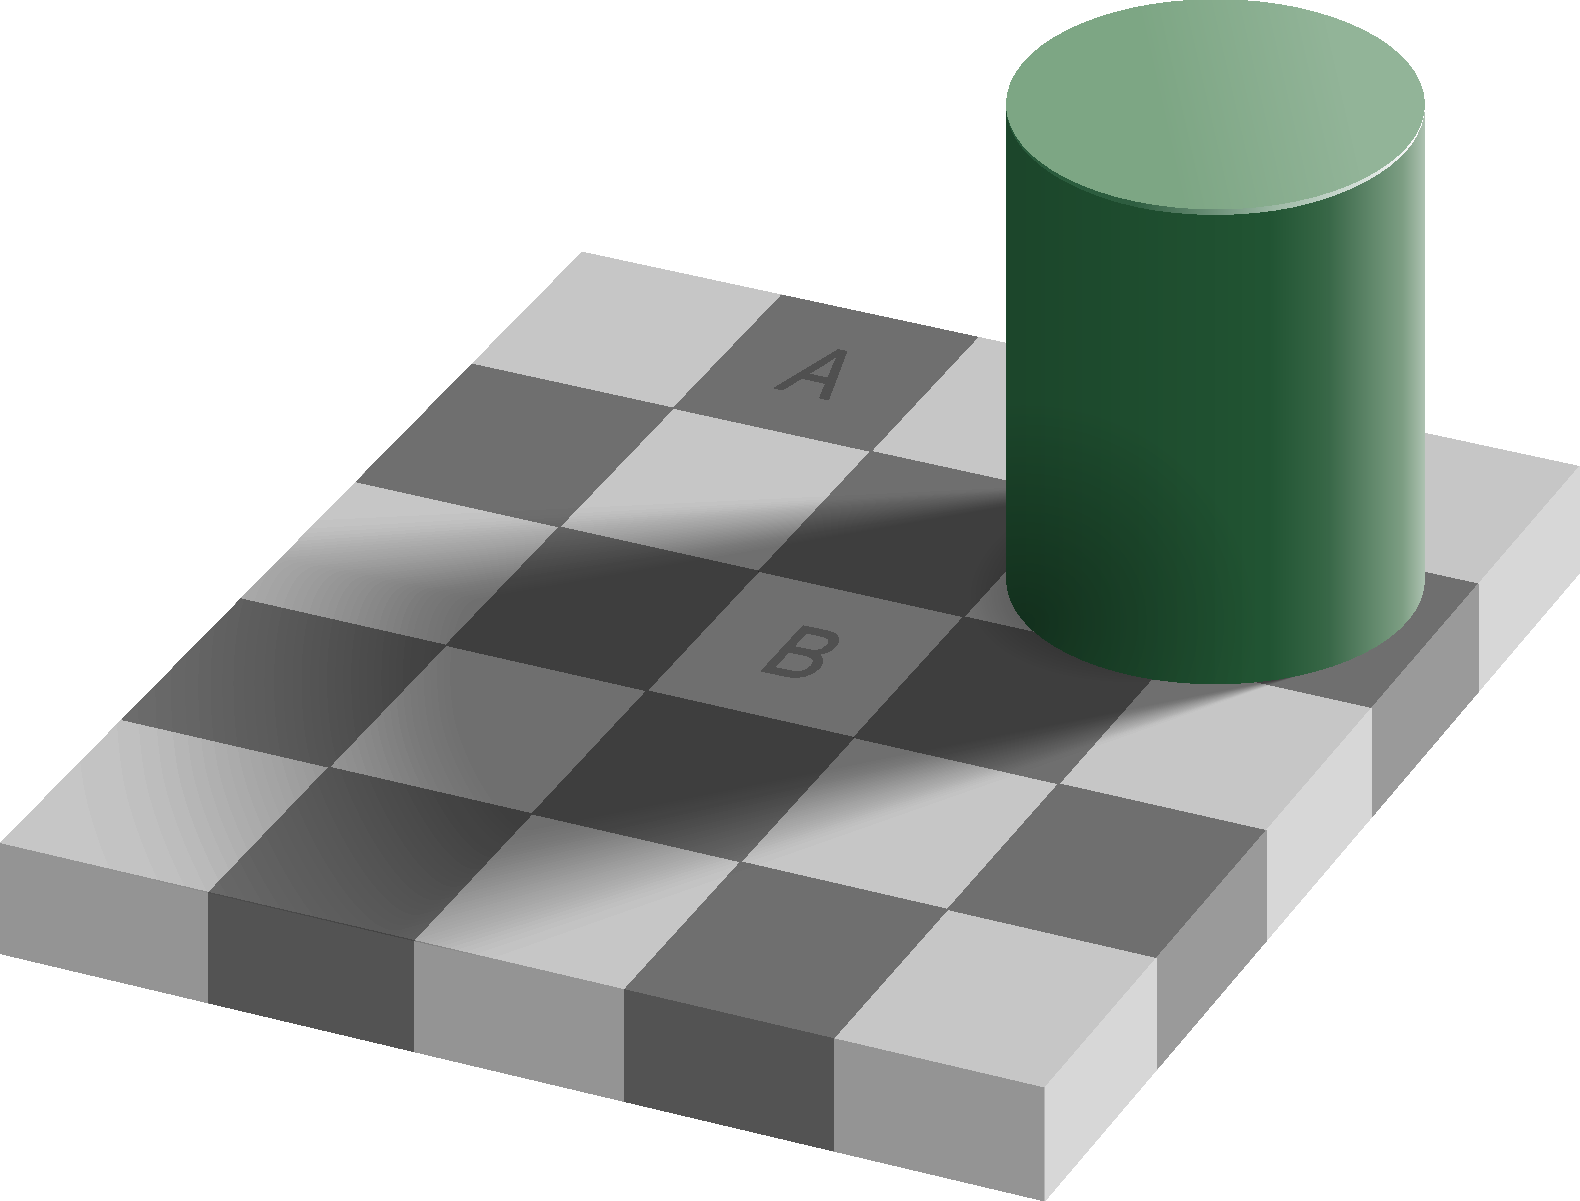
\includegraphics[width=7.4cm]{checker_shadow.pdf}};
  \begin{scope}[x={(im.south east)}, y={(im.north west)}, visible on=<2->]
    \fill[checkgray] (0.499,0.69) -- (0.547,0.69) -- (0.534,0.456) -- (0.486,0.456) -- cycle;
  \end{scope}
\end{tikzpicture}

    \end{column}
    \begin{column}{0.42\textwidth}
      \begin{itemize}
        \item Ի՞նչ գրեցիր սկզբում. A, թե B
        \item<2-> A-ն ու B-ն \textbf{նույն գույնն են}. միացնենք նույն մոխրագույնով
        \item<3-> Ուղեղը «գիտի», որ B-ն ստվերում է, ու ինքը «բացացնում» է այն
      \end{itemize}
      \onslide<3->{%
      \begin{card}[colback=butter!45!cream]
        \small Պատասխանը գիտես, բայց B-ն դեռ \textbf{բաց} է թվում։
      \end{card}}
    \end{column}
  \end{columns}
  \source{Edward H. Adelson, 1995}
\end{frame}

\begin{frame}{Ինչն է որտեղ, ու ով է դա}
  \begin{columns}[c]
    \begin{column}{0.5\textwidth}
      \centering
      \begin{tikzpicture}
        \path[use as bounding box] (-3.6,-2.4) rectangle (3.6,2.4);
        \begin{scope}[scale=0.66]
          \brainlobes{lavender!40!cream}{mint!45!cream}{peach!45!cream}{butter!80!cream}
          \fill[amRed, opacity=0.55] (3.0,-0.15) ellipse (0.3 and 0.55);
          \fill[amBlue, opacity=0.5, visible on=<2->] (1.4,1.6) ellipse (0.8 and 0.45);
          \fill[amOrange, opacity=0.8, visible on=<3->] (0.4,-1.05) ellipse (1.0 and 0.25);
          \node[wpill=amRed] at (3.6,-1.95) {տեսողական կեղև};
          \node[wpill=amBlue, visible on=<2->] at (1.6,3.05) {որտե՞ղ է};
          \node[wpill=amOrange!85!black, visible on=<3->] at (-1.5,-2.65) {ի՞նչ է, ո՞վ է};
        \end{scope}
      \end{tikzpicture}
    \end{column}
    \begin{column}{0.46\textwidth}
      \begin{itemize}
        \item Առաջնային կեղևից հեռու՝ ավելի \textbf{նեղ մասնագիտացում}
        \item<2-> Գագաթային բիլթը՝ \textbf{տարածությունը}
        \item<3-> Քունքային բլթի ստորին մասը՝ \textbf{առարկաներն ու դեմքերը}
      \end{itemize}
      \onslide<4->{%
      \begin{card}[colback=brainpink!25!cardwhite]
        \small Կա հատուկ մաս \textbf{դեմքերի} համար, ու դեմք ենք տեսնում ամենուր, նույնիսկ տոստի վրա։
      \end{card}}
    \end{column}
  \end{columns}
\end{frame}

\begin{frame}{3D՝ հարթ պատկերից}
  \begin{columns}[T]
    \begin{column}{0.5\textwidth}
      \begin{itemize}
        \item Ցանցաթաղանթը \textbf{հարթ} է, ինչպես գրատախտակը, իսկ մենք տեսնում ենք 3D
        \item<2-> Երկու աչքը տեսնում են մի քիչ \textbf{տարբեր} պատկերներ, ու ուղեղը դրանից հաշվում է խորությունը
      \end{itemize}
      \onslide<3->{%
      \begin{tryit}
        Բութ մատդ պահիր դեմքիդ առաջ ու հերթով փակիր աչքերդ. մատը «ցատկում» է։
      \end{tryit}}
    \end{column}
    \begin{column}{0.46\textwidth}
      \centering
      \onslide<4->{%
      \begin{meme}[6.3cm]{math_lady.jpg}
        \memecap[text width=4.8cm]{0.5}{0.88}{երկու հարթ պատկեր $\rightarrow$ 3D աշխարհ}
      \end{meme}}
    \end{column}
  \end{columns}
\end{frame}

\begin{frame}{Մեկ աչքով էլ է ստացվում}
  \begin{columns}[c]
    \begin{column}{0.54\textwidth}
      \centering
      % Depth cues that work with one eye: occlusion (the tree hides part of the house), texture (grass
% detail fades with distance) and lines converging into the distance (the road). Tags on slides 2-4.
\begin{tikzpicture}
  \path[use as bounding box] (-3.9,-2.15) rectangle (3.9,2.05);
  \begin{scope}
    \clip[rounded corners=3mm] (-3.8,-2.1) rectangle (3.8,2.0);
    \fill[lavender!35!cardwhite] (-3.8,0.75) rectangle (3.8,2.0);
    \fill[mint!55!cardwhite] (-3.8,-2.1) rectangle (3.8,0.75);
    % grass texture: big and sparse near, tiny and dense far
    \foreach \y/\s/\d in {-1.9/0.09/0.55, -1.45/0.07/0.45, -1.05/0.055/0.36, -0.7/0.04/0.28, -0.4/0.03/0.21, -0.15/0.022/0.16, 0.08/0.016/0.12, 0.28/0.012/0.09, 0.46/0.009/0.07}{
      \pgfmathtruncatemacro{\grassn}{7.6/\d}
      \foreach \k in {0,...,\grassn}{\fill[mintdark!70] (-3.8+\k*\d,\y) circle (\s);}}
    % road converging to the horizon
    \fill[plum!25!cardwhite] (-2.1,-2.1) -- (2.1,-2.1) -- (0.08,0.75) -- (-0.08,0.75) -- cycle;
    \draw[plum!70, line width=0.9pt] (-2.1,-2.1) -- (-0.08,0.75) (2.1,-2.1) -- (0.08,0.75);
    \foreach \a/\b in {-2.0/-1.45, -1.05/-0.68, -0.35/-0.1, 0.12/0.28, 0.42/0.52, 0.6/0.66}{
      \draw[butter!90!amOrange, line width=1.6pt] (0,\a) -- (0,\b);}
    % house, partly hidden by a tree
    \filldraw[fill=peach, draw=plum, line width=0.7pt] (1.6,0.35) rectangle (2.6,1.15);
    \filldraw[fill=plum!70, draw=plum, line width=0.7pt] (1.5,1.15) -- (2.1,1.6) -- (2.7,1.15) -- cycle;
    \node at (1.7,0.85) {\bigemoji[1.2cm]{tree}};
    % trees getting smaller along the road
    \foreach \x/\y/\h in {-2.9/-1.0/1.1, -1.85/-0.05/0.7, -1.15/0.45/0.45, -0.6/0.72/0.28}{\node at (\x,\y) {\bigemoji[\h cm]{tree}};}
  \end{scope}
  \draw[plum, line width=0.9pt, rounded corners=3mm] (-3.8,-2.1) rectangle (3.8,2.0);
  % tags
  \node[visible on=<2->, wpill=amRed] at (2.85,1.75) {1 ծածկում};
  \node[visible on=<3->, wpill=amBlue] at (-2.75,-1.8) {2 մանրամասներ};
  \node[visible on=<4->, wpill=amOrange!85!black] at (2.2,-1.8) {3 զուգահեռները հատվում են};
\end{tikzpicture}

    \end{column}
    \begin{column}{0.42\textwidth}
      \begin{itemize}
        \item Մի աչքով աշխարհը հարթ չի դառնում. ուղեղն օգտագործում է պատկերի \textbf{նշանները}
        \item<5-> Բըրնեթը ճանաչում էր միաչյա հաջողակ \textbf{ատամնաբույժի}
      \end{itemize}
      \onslide<4->{%
      \begin{scienceupdate}
        Գրքում 3-րդը կոչվում է convergence. ճիշտ տերմինը \textbf{գծային հեռանկարն} է։
      \end{scienceupdate}}
    \end{column}
  \end{columns}
\end{frame}

\begin{frame}{3D կինո}
  \centering
  % 3D cinema: two slightly shifted pictures on one screen; the glasses let each eye see only one of them;
% the brain reads the difference as depth. Reveals in 3 steps (use inside a frame).
\begin{tikzpicture}
  \path[use as bounding box] (-6.6,-1.6) rectangle (6.6,1.6);
  % screen with two overlapping pictures
  \filldraw[fill=cardwhite, draw=plum, line width=0.9pt, rounded corners=1.5mm] (-6.4,-1.1) rectangle (-3.4,1.1);
  \fill[amRed, opacity=0.55] (-5.05,0) circle (0.55);
  \fill[cyan!70!amBlue, opacity=0.55] (-4.75,0) circle (0.55);
  \node[font=\scriptsize, text=plum, align=center] at (-4.9,-1.4) {էկրանին՝ երկու պատկեր};
  % glasses
  \begin{scope}[visible on=<2->]
    \draw[warr] (-3.2,0) -- (-2.3,0);
    \filldraw[fill=amRed, fill opacity=0.5, draw=plum, line width=1pt, rounded corners=2mm] (-2.1,-0.35) rectangle (-1.2,0.35);
    \filldraw[fill=cyan!70!amBlue, fill opacity=0.5, draw=plum, line width=1pt, rounded corners=2mm] (-0.9,-0.35) rectangle (0.0,0.35);
    \draw[plum, line width=1pt] (-1.2,0.1) -- (-0.9,0.1);
    \node[font=\scriptsize, text=plum, align=center] at (-1.05,-1.4) {ակնոցը ամեն աչքին\\ թողնում է մեկը};
  \end{scope}
  % each eye gets its own picture
  \begin{scope}[visible on=<2->]
    \draw[warr] (0.2,0) -- (0.9,0);
    \node[draw=plum, line width=0.8pt, fill=cardwhite, rounded corners=1.5mm, minimum size=0.9cm] (le) at (1.5,0.55) {};
    \fill[amRed, opacity=0.55] (1.45,0.55) circle (0.3);
    \node[draw=plum, line width=0.8pt, fill=cardwhite, rounded corners=1.5mm, minimum size=0.9cm] (re) at (1.5,-0.55) {};
    \fill[cyan!70!amBlue, opacity=0.55] (1.6,-0.55) circle (0.3);
    \node[font=\scriptsize, text=plum, anchor=east] at (0.98,0.55) {\emoji{eye}};
    \node[font=\scriptsize, text=plum, anchor=east] at (0.98,-0.55) {\emoji{eye}};
  \end{scope}
  % the brain sees depth
  \begin{scope}[visible on=<3->]
    \draw[warr] (2.2,0) -- (3.0,0);
    \node at (3.75,0) {\mascot[1.5cm]{happy}};
    \node[draw=plum, line width=1pt, fill=butter, rounded corners=2mm, font=\blackfont\small, text=plum, rotate=8]
      at (5.6,0.55) {3D!};
    \node[font=\scriptsize, text=plum, align=center] at (5.2,-0.85) {տարբերությունը\\ = խորություն};
  \end{scope}
\end{tikzpicture}
\par\bigskip
  \begin{columns}[T]
    \begin{column}{0.47\textwidth}
      \small Սովորական կինոյում էլ կան խորության նշանները, բայց մենք գիտենք, որ էկրանը հարթ է։
    \end{column}
    \begin{column}{0.47\textwidth}
      \onslide<3->{\small 3D ակնոցով ամեն աչք իր պատկերն է ստանում, պատկերը «դուրս է թռչում» էկրանից, ու տոմսի համար \textbf{կրկնակի} ենք վճարում։}
    \end{column}
  \end{columns}
\end{frame}

\begin{frame}{Երկու դեմք, թե՞ ծաղկաման}
  \begin{columns}[c]
    \begin{column}{0.42\textwidth}
      \centering
      % Rubin's vase: two faces in profile looking at each other, or one vase between them.
% The vase is drawn in plum; the faces are the cream background. No reveals.
\begin{tikzpicture}[scale=0.85]
  % x = half-width of the vase (the distance from the centre line to each face's profile), top to bottom:
  % forehead, brow, eye, nose tip (narrowest), lips, chin, neck
  \fill[cardwhite] (-2.4,-2.75) rectangle (2.4,2.75);
  \fill[plum] plot[smooth, tension=0.55] coordinates {(1.55,2.6) (1.3,2.25) (0.95,1.85) (0.72,1.5) (0.86,1.18)
      (0.82,0.95) (0.5,0.62) (0.28,0.38) (0.42,0.2) (0.52,0.05) (0.4,-0.12) (0.48,-0.28) (0.38,-0.44)
      (0.58,-0.68) (0.46,-0.98) (0.42,-1.2) (0.75,-1.5) (1.05,-1.85) (1.2,-2.25) (1.25,-2.6)}
    -- (-1.25,-2.6)
    -- plot[smooth, tension=0.55] coordinates {(-1.25,-2.6) (-1.2,-2.25) (-1.05,-1.85) (-0.75,-1.5) (-0.42,-1.2)
      (-0.46,-0.98) (-0.58,-0.68) (-0.38,-0.44) (-0.48,-0.28) (-0.4,-0.12) (-0.52,0.05) (-0.42,0.2) (-0.28,0.38)
      (-0.5,0.62) (-0.82,0.95) (-0.86,1.18) (-0.72,1.5) (-0.95,1.85) (-1.3,2.25) (-1.55,2.6)} -- cycle;
  \draw[plum, line width=1pt] (-2.4,-2.75) rectangle (2.4,2.75);
\end{tikzpicture}

    \end{column}
    \begin{column}{0.54\textwidth}
      \begin{chatbox}
        Ի՞նչ տեսար \textbf{առաջինը}՝ ծաղկաման, թե՞ երկու դեմք։ Գրիր չաթում։
      \end{chatbox}
      \vspace{1mm}
      \onslide<2->{%
      \begin{itemize}
        \item Երկու պատասխանն էլ \textbf{ճիշտ} են, բայց միաժամանակ չես տեսնում
        \item Ուղեղը երկիմաստություն չի սիրում ու \textbf{ընտրում է մեկը}
        \item Բայց կարող է կարծիքը փոխել. փորձիր
      \end{itemize}}
    \end{column}
  \end{columns}
\end{frame}

\begin{frame}{Սառցաբեկորի գագաթը}
  \begin{columns}[c]
    \begin{column}{0.56\textwidth}
      \begin{card}\emoji{bread}\ \textbf{Դեմքեր}՝ քունքային կեղևի դեմքերի հատվածը\end{card}
      \begin{card}\emoji{palette}\ \textbf{Գույներ}՝ երկրորդային տեսողական կեղևը շփոթվում է ֆոնից\end{card}
      \begin{card}\emoji{question}\ \textbf{Երկիմաստություն}՝ ուղեղը ընտրում է մեկ տարբերակ\end{card}
    \end{column}
    \begin{column}{0.4\textwidth}
      \onslide<2->{%
      \begin{bookquote}
        Սա տեսողական համակարգի սառցաբեկորի գագաթն է միայն։ Իսկ խորությունը կարող ես տեսնել միայն այն պատճառով, որ տեսողական համակարգն այդքան բարդ է։
      \end{bookquote}}
    \end{column}
  \end{columns}
\end{frame}

% ===== Section 4: Why your ears are burning (attention, ~18 min) =====
\topicopener{headphones}{Ուշադրություն}{Ինչու են ականջներդ «այրվում»}{Ուշադրության ուժն ու թուլությունները, ու ինչու չես կարող չլսել ուրիշի խոսակցությունը}{thinking}

\begin{frame}{Ուղեղը չի կարող ամեն ինչ մշակել}
  \begin{columns}[T]
    \begin{column}{0.52\textwidth}
      \begin{itemize}
        \item Զգայարանները անընդհատ \textbf{հսկայական} տեղեկություն են ուղարկում
        \item<2-> Ուղեղը շատ «թանկ» օրգան է. չորացող ներկին նայելու վրա ռեսուրս վատնելը անիմաստ է
        \item<3-> \textbf{Ուշադրությունը} որոշում է, թե ինչը կնկատենք։ Ու, որ հաճախ ավելի կարևոր է, ինչը \textbf{չենք նկատի}
      \end{itemize}
    \end{column}
    \begin{column}{0.44\textwidth}
      \onslide<4->{%
      \begin{card}[colback=butter!45!cream]
        {\blackfont Երկու հարց}\par\smallskip
        \emoji{battery}\ \textbf{Որքա՞ն} ենք կարողանում մշակել\par\smallskip
        \emoji{target}\ \textbf{Ի՞նչն է} որոշում, թե ուր ուղղվի ուշադրությունը
      \end{card}}
    \end{column}
  \end{columns}
\end{frame}

\begin{frame}{Բոլորը միանգամից խոսում են}
  \centering
  % Cherry's dichotic listening: a different stream of words in each ear; repeat the left one.
% What people remember from the right ear appears on slide 2 (use inside a frame).
\begin{tikzpicture}
  \path[use as bounding box] (-6.4,-1.65) rectangle (6.4,1.8);
  \node at (0,0.05) {\mascot[2.3cm]{thinking}};
  % headphones
  \draw[plum, line width=2.2pt] (-1.15,0.15) .. controls (-1.1,1.75) and (1.1,1.75) .. (1.15,0.15);
  \filldraw[fill=amBlue, draw=plum, line width=1pt, rounded corners=1.5mm] (-1.42,-0.45) rectangle (-0.98,0.4);
  \filldraw[fill=plum!45!cream, draw=plum, line width=1pt, rounded corners=1.5mm] (0.98,-0.45) rectangle (1.42,0.4);
  % left ear: the stream to repeat
  \node[chatmsg=3.7cm, fill=amBlue!12!cardwhite, align=center] (L) at (-4.2,0.55) {«խնձոր... սեղան... ամպ... գետ...»};
  \node[wpill=amBlue] at (-4.2,1.5) {ձախ ականջ. կրկնիր բարձրաձայն};
  \draw[warr=amBlue] (L.east) -- (-1.5,0.1);
  % right ear: the ignored stream
  \node[chatmsg=3.7cm, fill=cardwhite, align=center, text=plum!60!cream] (R) at (4.2,0.55) {«շուն... լամպ... կոշիկ... ձյուն...»};
  \node[wpill=plum!60] at (4.2,1.5) {աջ ականջ. անտեսիր};
  \draw[warr=plum!50] (R.west) -- (1.5,0.1);
  % what is left of the ignored stream
  \node[visible on=<2->, draw=pinkdark, line width=1.2pt, fill=blush!15!cardwhite, rounded corners=2.5mm,
        text width=4.0cm, align=center, font=\small, text=plum, inner sep=4pt] at (4.2,-0.95)
    {Աջից հիշում են միայն՝ \textbf{տղամարդ էր, թե կին}։ Նույնիսկ \textbf{լեզուն} չէին նկատում};
\end{tikzpicture}
\par\smallskip
  \begin{columns}[T]
    \begin{column}{0.47\textwidth}
      \small 1953. Քոլին Չերին (Colin Cherry) մարդկանց երկու ականջին տարբեր բառեր էր տալիս (dichotic listening)։
    \end{column}
    \begin{column}{0.47\textwidth}
      \onslide<3->{\small Եզրակացություն՝ ուշադրությունը \textbf{նեղ բկով շիշ} է (bottleneck)։ Հեռադիտակի պես. մի փոքր կտորը մանրամասն, մնացածը՝ ոչինչ։}
    \end{column}
  \end{columns}
\end{frame}

\begin{frame}{Բայց ուղեղը լսում էր}
  \begin{columns}[T]
    \begin{column}{0.52\textwidth}
      \begin{itemize}
        \item 1975. Ֆոն Ռայթն (von Wright) ու գործընկերները մարդկանց սովորեցրին որոշ բառերից հետո \textbf{էլեկտրական հարված} սպասել \emoji{lightning}
        \item<2-> Հետո նույն բառերը հնչեցին \textbf{անտեսվող} ականջում
        \item<3-> Մարդիկ բառերը չէին նկատում, բայց մարմինը \textbf{վախով} էր արձագանքում
      \end{itemize}
    \end{column}
    \begin{column}{0.44\textwidth}
      \onslide<4->{%
      \begin{card}[colback=brainpink!25!cardwhite]
        Ուրեմն ուղեղը մշակում էր նաև «մյուս» ականջը, պարզապես տեղեկությունը \textbf{գիտակցությանը չէր հասնում}։ Շշի բկի մոդելը չի աշխատում։
      \end{card}}
    \end{column}
  \end{columns}
\end{frame}

\begin{frame}{Կոկտեյլի երեկույթի էֆեկտ}
  \begin{columns}[T]
    \begin{column}{0.5\textwidth}
      \begin{poll}
        Բարձրացրու ձեռքդ, եթե աղմկոտ սենյակում \textbf{լսել ես անունդ} ուրիշների խոսակցությունից ու միանգամից «միացել» նրանց զրույցին։
      \end{poll}
      \vspace{1mm}
      \onslide<3->{\small Սա կոչվում է \textbf{կոկտեյլի երեկույթի էֆեկտ} (cocktail party effect). «որովհետև հոգեբանները նրբաճաշակ մարդիկ են»։}
    \end{column}
    \begin{column}{0.46\textwidth}
      \onslide<2->{%
      \begin{card}
        \emoji{party}\ Հարսանիք։ Սեղանի մոտ խոսում ես ֆուտբոլից կամ նեխուրից։ Հարևան խմբում ինչ-որ մեկն ասում է \textbf{քո անունը}, ու հետո՝ «...իսկական մաշկի վատնում է»։\par\smallskip
        Ու հիմա դու լսում ես միայն \textbf{նրանց} ու մտածում, թե ինչու ես այդ մարդուն քավոր ընտրել։
      \end{card}}
    \end{column}
  \end{columns}
\end{frame}

\begin{frame}{Հարսանիքում}
  \centering
  \begin{meme}[6.9cm]{monkey_puppet.jpg}
    \memecap[text width=5.8cm, font=\blackfont\normalsize]{0.5}{0.84}{Հարևան սեղանից ինչ-որ մեկը ասում է իմ անունը}
    \memecap{0.27}{0.08}{ես, իբր չեմ լսում}
  \end{meme}
\end{frame}

\begin{frame}{Ուշադրությունը՝ սահմանափակ բյուջե}
  \centering
  % Kahneman's capacity model: attention as a limited budget shared between tasks. Each task takes a
% share; the fourth one does not fit. Segments appear on slides 1-4 (use inside a frame).
\begin{tikzpicture}[seg/.style={draw=plum, line width=0.8pt, font=\small, text=plum, align=center, minimum height=0.9cm}]
  \path[use as bounding box] (-0.2,-1.0) rectangle (12.4,1.2);
  \draw[plum, line width=1.4pt, rounded corners=2mm] (0,-0.5) rectangle (9.6,0.5);
  \node[font=\blackfont\scriptsize, text=plum, anchor=south west] at (0,0.55) {ուշադրության «բյուջեն»};
  \node[seg, fill=mint!60!cardwhite, minimum width=4.2cm, anchor=west] at (0.05,0) {\emoji{car}\ ճանապարհ};
  \node[seg, fill=butter!70!cardwhite, minimum width=3.0cm, anchor=west, visible on=<2->] at (4.25,0) {\emoji{speech}\ զրույց};
  \node[seg, fill=peach!60!cardwhite, minimum width=2.25cm, anchor=west, visible on=<3->] at (7.25,0) {\emoji{musical}\ ռադիո};
  \node[seg, fill=blush!50!cardwhite, draw=pinkdark, minimum width=2.6cm, anchor=west, visible on=<4->] at (9.7,0) {\emoji{phone}\ հեռախոս};
  \node[visible on=<4->, font=\blackfont\scriptsize, text=pinkdark] at (11.0,-0.8) {չի տեղավորվում};
\end{tikzpicture}
\par\smallskip
  \begin{columns}[T]
    \begin{column}{0.47\textwidth}
      \begin{card}[colback=lavender!35!cardwhite]
        \small\textbf{Ռեսուրսի մոդել} (Kahneman, 1973). ուշադրությունը կարելի է \textbf{բաժանել} մի քանի բանի միջև, քանի դեռ ռեսուրսը չի սպառվել։
      \end{card}
    \end{column}
    \begin{column}{0.47\textwidth}
      \onslide<5->{%
      \begin{card}[colback=mint!35!cardwhite]
        \small Ինչու՞ է այդքան քիչ։ Ուշադրությունը տեղեկություն է տալիս \textbf{կարճաժամկետ հիշողությանը}, իսկ այն տեղավորում է մոտ 4 բան (վեբինար 1)։
      \end{card}}
    \end{column}
  \end{columns}
\end{frame}

\begin{frame}{Հեռախոսով, բայց առանց ձեռքերի}
  \begin{columns}[c]
    \begin{column}{0.5\textwidth}
      \begin{itemize}
        \item Շատ երկրներում վարելիս հեռախոսը ձեռքում պահել չի կարելի, իսկ առանց ձեռքերի (hands-free)՝ կարելի է
        \item<2-> Յուտայի համալսարան, 2013. hands-free-ն \textbf{նույնքան վատ է}. արձագանքը, շուրջը նայելը, նշանները նկատելը նույնքան են տուժում
        \item<3-> Ըստ Բըրնեթի՝ ռադիոն փոխելն ու ուղևորի հետ զրույցն էլ են նույնքան շեղում
      \end{itemize}
    \end{column}
    \begin{column}{0.46\textwidth}
      \centering
      \onslide<4->{%
      \begin{meme}[5.6cm]{left_exit.jpg}
        \memecap{0.45}{0.83}{ճանապարհ}
        \memecap{0.62}{0.69}{նոր հաղորդագրություն}
        \memecap{0.48}{0.12}{ուշադրությունս}
      \end{meme}}
    \end{column}
  \end{columns}
\end{frame}

\begin{frame}{Ինչպե՞ս ենք ընդհանրապես վարում}
  \begin{columns}[c]
    \begin{column}{0.58\textwidth}
      \begin{itemize}
        \item Սկսնակի համար վարելը սարսափելի ծանր է
        \item<2-> Բայց կրկնությունից հետո այն դառնում է \textbf{պրոցեդուրային հիշողություն} (վեբինար 1), ու ենթագիտակցությունն է վարում «առանց մտածելու»
        \item<3-> Բայց ոչ ամբողջովին. մյուս վարորդներն ու վտանգները ամեն անգամ նոր են, ու դրանց համար \textbf{գիտակցված ուշադրություն} է պետք
      \end{itemize}
    \end{column}
    \begin{column}{0.38\textwidth}
      \centering
      \bigemoji[1.6cm]{car}\par\medskip
      \onslide<3->{%
      \begin{card}[colback=peach!40!cardwhite]
        \small Աչքերդ կարող են ճանապարհին լինել, բայց եթե չես «նայում» նրանց տվածին, \textbf{անիմաստ} է։
      \end{card}}
    \end{column}
  \end{columns}
\end{frame}

\begin{frame}{Որտե՞ղ է ուշադրությունը}
  \begin{columns}[c]
    \begin{column}{0.48\textwidth}
      \centering
      \begin{tikzpicture}
        \path[use as bounding box] (-3.1,-1.8) rectangle (3.1,1.9);
        \begin{scope}[scale=0.56]
          \brainlobes{lavender!40!cream}{mint!40!cream}{peach!45!cream}{butter!80!cream}
          \fill[amBlue, opacity=0.55] (-2.3,1.0) ellipse (0.8 and 0.65);
          \draw[amOrange!85!black, line width=1.4pt, dashed, visible on=<2->] (-0.9,0.9) .. controls (-0.2,1.45) and (0.8,1.35) .. (1.3,0.95);
          \node[wpill=amBlue] at (-2.3,2.75) {նախաճակատային կեղև};
          \node[wpill=amOrange!85!black, visible on=<2->] at (1.7,-2.95) {առաջային գոտկային կեղև (ներսում)};
        \end{scope}
      \end{tikzpicture}
    \end{column}
    \begin{column}{0.48\textwidth}
      \begin{itemize}
        \item \textbf{Նախաճակատային կեղև}. այնտեղ է կարճաժամկետ հիշողությունը
        \item<2-> \textbf{Առաջային գոտկային կեղև} (anterior cingulate)
      \end{itemize}
      \onslide<3->{\small Համակարգերը \textbf{ցրված} են ուղեղով մեկ։\par\smallskip}
      \onslide<4->{%
      \begin{scienceupdate}
        Գրքում՝ «քունքային բլթի խորքում»։ Իրականում այն կիսագնդերի \textbf{ներքին} մակերեսին է։
      \end{scienceupdate}}
    \end{column}
  \end{columns}
  \onslide<4->{\source{Bush, Luu \& Posner, Trends Cogn. Sci., 2000}}
\end{frame}

\begin{frame}{Ներքևից վեր և վերևից ներքև}
  \begin{columns}[T]
    \begin{column}{0.47\textwidth}
      \begin{card}[colback=peach!40!cardwhite]
        \emoji[1.3em]{bell}\ {\blackfont Ներքևից վեր} (bottom-up)\par\smallskip
        Դրսի ինչ-որ բան \textbf{ինքն է} գրավում ուշադրությունը։ Անունդ հնչեց, ու դու արդեն լսում ես։
      \end{card}
    \end{column}
    \begin{column}{0.47\textwidth}
      \onslide<2->{%
      \begin{card}[colback=lavender!40!cardwhite]
        \emoji[1.3em]{brain}\ {\blackfont Վերևից ներքև} (top-down)\par\smallskip
        \textbf{Դու ես} որոշում, թե ուր նայել ու ինչ լսել։ Ուզում ես իմանալ, թե ինչ են ասում քո մասին։
      \end{card}}
    \end{column}
  \end{columns}
  \vspace{2mm}
  \onslide<3->{%
  \begin{card}[colback=mint!35!cardwhite]
    \small\emoji{headphones}\ Ինչպե՞ս ենք «ուղղում» ականջները։ 2012-ին Չանգն ու Մեսգարանին երեք պացիենտի լսողական կեղևում տեսան, որ ակտիվություն է տալիս միայն այն ձայնը, որին մարդը \textbf{ուշադիր է}։ Ուղեղն իսկապես կարող է «անջատել» ձանձրալի զրուցակցին՝ ոզնիներ դիտելու իր հոբբիով։
  \end{card}}
  \onslide<3->{\source{Mesgarani \& Chang, Nature, 2012}}
\end{frame}

\begin{frame}{Աչքերը՝ ուշադրության գլխավոր գործիքը}
  \begin{columns}[T]
    \begin{column}{0.47\textwidth}
      \begin{card}[colback=lavender!40!cardwhite]
        \emoji[1.3em]{target}\ {\blackfont Նպատակով}\par\smallskip
        Տեսար «ԱՆՎՃԱՐ ԲԵԿՈՆ» ցուցանակը, ու աչքերդ \textbf{դու ես} ուղղում այնտեղ։
      \end{card}
    \end{column}
    \begin{column}{0.47\textwidth}
      \onslide<2->{%
      \begin{card}[colback=peach!40!cardwhite]
        \emoji[1.3em]{tiger}\ {\blackfont Ինքնաբերաբար}\par\smallskip
        Վագրի մռնչյուն, ճյուղի ճռռոց. ուշադրությունը շրջվում է \textbf{նախքան} գիտակցությունը կհասկանա։
      \end{card}}
    \end{column}
  \end{columns}
  \vspace{2mm}
  \onslide<3->{%
  \begin{scienceupdate}[width=0.86\textwidth]
    Գրքում սրանք կոչվում են «overt» ու «covert»։ Այսօր overt-ը նշանակում է \textbf{աչքերը շարժելով}, covert-ը՝ առանց շարժելու։
  \end{scienceupdate}}
  \onslide<3->{\source{Posner, Q. J. Exp. Psychol., 1980}}
\end{frame}

\begin{frame}{Ծնողը, հեռուստացույցը ու աղբը}
  \centering
  % Burnett's parent-and-bins version of how attention shifts to something important: the posterior
% parietal cortex disengages, the superior colliculus moves, the pulvinar re-engages. Steps on slides 1-3.
\begin{tikzpicture}[
    stage/.style={draw=plum, line width=0.9pt, rounded corners=3mm, text width=3.6cm, align=center,
      font=\small, text=plum, inner sep=3.5pt, minimum height=2.7cm},
  ]
  \node[stage, fill=lavender!40!cardwhite] (a) at (0,0)
    {\bigemoji[0.7cm]{tv}\\[1mm] \textbf{Անջատել}\\ {\scriptsize հետին գագաթային կեղև}\\[1mm] Ծնողն անջատում է հեռուստացույցը};
  \node[stage, fill=mint!40!cardwhite, visible on=<2->] (b) at (4.6,0)
    {\bigemoji[0.7cm]{walking}\\[1mm] \textbf{Տեղափոխել}\\ {\scriptsize վերին թմբիկներ (superior colliculus)}\\[1mm] Երեխային տանում է խոհանոց};
  \node[stage, fill=peach!45!cardwhite, visible on=<3->] (c) at (9.2,0)
    {\bigemoji[0.7cm]{wastebasket}\\[1mm] \textbf{Նորից միացնել}\\ {\scriptsize թալամուսի բարձիկ (pulvinar)}\\[1mm] Աղբի տոպրակը տալիս է ձեռքը ու հրում դեպի դուռը};
  \draw[warr, visible on=<2->] (a) -- (b);
  \draw[warr, visible on=<3->] (b) -- (c);
\end{tikzpicture}
\par\smallskip
  \onslide<4->{%
  \begin{card}[width=0.9\textwidth, colback=butter!40!cream]
    \centering Այս համակարգը կարող է \textbf{վերագրել} գիտակցականին։ Անծանոթ ուրվագիծը կարող է հարձակվող լինել։ Կամ ձանձրալի գործընկերը, որ պատմում է իր ոտքի սնկի մասին։
  \end{card}}
\end{frame}

\begin{frame}{Աչքի անկյունում՝ սարդ}
  \begin{columns}[c]
    \begin{column}{0.56\textwidth}
      \begin{itemize}
        \item Աշխատում ես, ու աչքիդ անկյունում ինչ-որ բան շարժվեց՝ մեծ \textbf{սարդի} չափ
        \item<2-> Չես նայում (հանկարծ իսկապես սարդ է), բայց շարունակում ես մտքով «հետևել» այդ անկյունին
        \item<3-> Ուշադրությունը \textbf{կապված չէ} աչքերի ուղղությանը
      \end{itemize}
    \end{column}
    \begin{column}{0.4\textwidth}
      \centering
      \bigemoji[1.2cm]{computer}\ \onslide<1->{\raisebox{-2mm}{\bigemoji[0.7cm]{spider}}}\par\medskip
      \onslide<4->{%
      \begin{card}[colback=lavender!35!cardwhite]
        \emoji{firework}\ Թե ինչն է «կարևոր», որոշում է համատեքստը։ Ամանորի գիշերը հրավառության ձայնը սովորական է. ավելի տարօրինակ կլիներ \textbf{լռությունը}։
      \end{card}}
    \end{column}
  \end{columns}
\end{frame}

\begin{frame}{Երկու բան միաժամանակ}
  \begin{columns}[c]
    \begin{column}{0.5\textwidth}
      \centering
      % A Posner cueing trial: look at the cross; an arrow cue points left; the target appears on the right
% (a wrong cue), so attention has to move. Slides: 1 = boxes, 2 = cue, 3 = target (use inside a frame).
\begin{tikzpicture}[scale=0.8]
  \path[use as bounding box] (-4.1,-1.3) rectangle (4.1,1.3);
  \filldraw[fill=cardwhite, draw=plum, line width=1pt, rounded corners=1mm] (-3.9,-0.9) rectangle (-2.1,0.9);
  \filldraw[fill=cardwhite, draw=plum, line width=1pt, rounded corners=1mm] (2.1,-0.9) rectangle (3.9,0.9);
  \draw[plum, line width=1.5pt] (-0.25,0) -- (0.25,0) (0,-0.25) -- (0,0.25);
  \draw[amBlue, line width=3pt, -{Stealth[length=4mm]}, visible on=<2->] (0.9,0.6) -- (-0.9,0.6);
  \node[visible on=<3->] at (3.0,0) {\bigemoji[1.1cm]{star}};
\end{tikzpicture}
\par\smallskip
      {\small Նայիր \textbf{+}-ին։ Սլաքը ցույց է տալիս, թե որտեղ կհայտնվի աստղը... երբեմն սխալ}
    \end{column}
    \begin{column}{0.46\textwidth}
      \begin{itemize}
        \item<4-> Մայքլ Պոզների (Michael Posner) թեստերում արդեն \textbf{երկու} հուշումը շատ է
        \item<5-> Տեսողական ու լսողական առաջադրանքները կարելի է բաժանել, բայց միայն պարզ «այո/ոչ»-ի դեպքում
        \item<6-> Բացառություն՝ երբ մեկը շատ վարժ է. փորձառու վարորդը զրուցում է, փորձառու մեքենագրողը թվաբանություն է անում
      \end{itemize}
    \end{column}
  \end{columns}
\end{frame}

\begin{frame}{Օձեր ու սարդեր. վայրկյանի մի մասում}
  \begin{columns}[T]
    \begin{column}{0.52\textwidth}
      \begin{itemize}
        \item Ուփսալայի համալսարան. մարդկանց ցույց էին տալիս օձերի ու սարդերի նկարներ \textbf{1/300 վայրկյանից} էլ կարճ
        \item<2-> Գիտակցորեն ճանաչելու համար պետք է մոտ \textbf{կես վայրկյան}
        \item<3-> Բայց ափերը միևնույն է \textbf{քրտնում} էին. անգիտակից ուշադրությունը վտանգը նկատում է նախքան գիտակցությունը կասի՝ «Հը՞, ի՞նչ»
      \end{itemize}
    \end{column}
    \begin{column}{0.44\textwidth}
      \centering
      \bigemoji[1.1cm]{snake}\ \bigemoji[1.1cm]{spider}\par\medskip
      \onslide<4->{%
      \begin{scienceupdate}
        Այս տիպի դասական փորձերում նկարը ցույց էին տալիս \textbf{30 միլիվայրկյան} (մոտ 1/33 վ), հետո՝ ծածկող պատկեր։ «1/300»-ը չկարողացանք հաստատել։
      \end{scienceupdate}}
    \end{column}
  \end{columns}
  \onslide<4->{\source{Öhman \& Soares, J. Abnorm. Psychol., 1994}}
\end{frame}

\begin{frame}{Դռան փորձը}
  \centering
  % Simons & Levin's door study in three panels: an experimenter asks a pedestrian for directions,
% two people carry a door between them, and a different experimenter is standing there afterwards.
% Panels on slides 1-3 (use inside a frame).
\begin{tikzpicture}[scale=0.84,
    panel/.style={draw=plum, line width=0.8pt, fill=cardwhite, rounded corners=2.5mm},
    plbl/.style={font=\scriptsize, text=plum, align=center, text width=3.1cm},
  ]
  \path[use as bounding box] (-0.1,-0.65) rectangle (12.6,2.85);
  \foreach \i/\s in {0/1, 1/2, 2/3}{
    \begin{scope}[xshift=\i*4.25cm, visible on=<\s->]
      \draw[panel] (0,0) rectangle (4.0,2.9);
      % pedestrian (right) with the map
      \fill[plum!70] (3.0,1.95) circle (0.24);
      \fill[plum!70, rounded corners=1.5mm] (2.72,0.35) rectangle (3.28,1.65);
      \filldraw[fill=butter, draw=plum, line width=0.6pt, rotate around={-12:(2.45,1.15)}] (2.15,0.9) rectangle (2.75,1.4);
    \end{scope}}
  % panel 1: experimenter A (blue)
  \fill[amBlue] (1.0,1.95) circle (0.24);
  \fill[plum] (0.78,2.05) rectangle (1.22,2.2);
  \fill[amBlue, rounded corners=1.5mm] (0.72,0.35) rectangle (1.28,1.65);
  \node[say, font=\scriptsize, callout absolute pointer={(1.2,2.0)}] at (1.9,2.55) {Ինչպե՞ս գնամ...};
  \node[plbl] at (2.0,-0.35) {հարցնում է ճանապարհը};
  % panel 2: the door
  \begin{scope}[xshift=4.25cm, visible on=<2->]
    \fill[amBlue] (1.0,1.95) circle (0.24);
    \fill[amBlue, rounded corners=1.5mm] (0.72,0.35) rectangle (1.28,1.65);
    \filldraw[fill=peachdark!70, draw=plum, line width=0.9pt] (1.55,0.2) rectangle (2.35,2.55);
    \fill[butter] (2.2,1.35) circle (0.06);
    \node[plbl] at (2.0,-0.35) {մեջտեղով դուռ են անցկացնում};
  \end{scope}
  % panel 3: experimenter B (orange, different hair)
  \begin{scope}[xshift=8.5cm, visible on=<3->]
    \fill[amOrange] (1.0,1.95) circle (0.24);
    \fill[peachdark] (0.74,2.1) .. controls (1.0,2.4) .. (1.26,2.1) -- cycle;
    \fill[amOrange, rounded corners=1.5mm] (0.68,0.35) rectangle (1.32,1.75);
    \node[say, font=\scriptsize, callout absolute pointer={(1.2,2.0)}] at (1.9,2.55) {...ու հետո՞};
    \node[plbl] at (2.0,-0.35) {ուրիշ մարդ է կանգնած};
  \end{scope}
\end{tikzpicture}
\par
  \begin{columns}[T]
    \begin{column}{0.47\textwidth}
      \begin{poll}
        Կնկատեի՞ր, որ դիմացդ \textbf{ուրիշ մարդ} է։ Բարձրացրու ձեռքդ, եթե այո։
      \end{poll}
    \end{column}
    \begin{column}{0.47\textwidth}
      \onslide<4->{%
      \begin{card}[colback=brainpink!25!cardwhite]
        \small 1998. Նկատել է \textbf{15-ից միայն 7-ը}։ Իսկ 50 ուսանողից բոլորն էին վստահ, որ կնկատեն։
      \end{card}}
    \end{column}
  \end{columns}
  \onslide<4->{\source{Simons \& Levin, Psychon. Bull. Rev., 1998}}
\end{frame}

\begin{frame}{«Դռան փորձ»}
  \begin{columns}[c]
    \begin{column}{0.56\textwidth}
      \begin{bookquote}
        Այն կոչվում է «դռան փորձ», որովհետև, ըստ երևույթին, ամենահետաքրքիրը դուռն է։ Գիտնականները տարօրինակ մարդիկ են։
      \end{bookquote}
    \end{column}
    \begin{column}{0.4\textwidth}
      \centering
      \bigemoji[1.8cm]{door}\par\medskip
      {\small Ու մի մանրուք հոդվածից. մարդկանց մեծ մասն այդ պահից նկատել էր միայն, որ դուռ տանողները \textbf{անքաղաքավարի} էին։}
    \end{column}
  \end{columns}
  \source{Simons \& Levin, 1998}
\end{frame}

\begin{frame}{Փոփոխության կուրություն}
  \begin{columns}[c]
    \begin{column}{0.66\textwidth}
      \centering
      % Change-blindness demo (flicker): scene with a chimney on slides 1, 5 and 8, without it on 3 and 7,
% a blank screen on 2, 4 and 6; slide 8 circles the change. Use inside a frame with 8 slides.
\begin{tikzpicture}[scale=0.9]
  \path[use as bounding box] (-5.2,-2.15) rectangle (5.2,2.15);
  \begin{scope}
    \clip[rounded corners=3mm] (-5.1,-2.1) rectangle (5.1,2.1);
    \fill[lavender!40!cardwhite] (-5.1,-2.1) rectangle (5.1,2.1);
    \fill[mint!60!cardwhite] (-5.1,-2.1) rectangle (5.1,-0.9);
    % sun and cloud
    \fill[amOrange!75] (3.9,1.45) circle (0.4);
    \fill[cardwhite] (-3.2,1.45) ellipse (0.75 and 0.3) (-2.7,1.6) ellipse (0.5 and 0.3);
    % house
    \only<1,2,4,5,6,8>{\filldraw[fill=peachdark!75, draw=plum, line width=0.8pt] (0.95,0.95) rectangle (1.3,1.65);}
    \filldraw[fill=peach, draw=plum, line width=0.8pt] (-0.4,-1.0) rectangle (1.9,0.55);
    \filldraw[fill=plum!70, draw=plum, line width=0.8pt] (-0.6,0.55) -- (0.75,1.55) -- (2.1,0.55) -- cycle;
    \filldraw[fill=butter, draw=plum, line width=0.7pt] (-0.1,-0.35) rectangle (0.45,0.2);
    \filldraw[fill=peachdark, draw=plum, line width=0.7pt] (0.95,-1.0) rectangle (1.45,-0.05);
    % tree, fence, car
    \fill[peachdark] (-2.75,-1.0) rectangle (-2.5,-0.2);
    \fill[mintdark] (-2.62,0.15) circle (0.62);
    \foreach \x in {-4.8,-4.4,...,-3.2}{\filldraw[fill=cardwhite, draw=plum, line width=0.5pt] (\x,-1.0) rectangle ++(0.18,0.6);}
    \draw[plum, line width=0.6pt] (-4.85,-0.65) -- (-3.0,-0.65);
    \node at (3.5,-1.15) {\bigemoji[0.9cm]{car}};
  \end{scope}
  \draw[plum, line width=0.9pt, rounded corners=3mm] (-5.1,-2.1) rectangle (5.1,2.1);
  % blank flashes
  \only<2,4,6>{\fill[cream] (-5.2,-2.15) rectangle (5.2,2.15);}
  % the answer
  \only<8>{\draw[amRed, line width=2pt] (1.12,1.3) circle (0.55);
    \node[wpill=amRed] at (2.6,1.75) {ծխնելույզը};}
\end{tikzpicture}

    \end{column}
    \begin{column}{0.3\textwidth}
      \begin{chatbox}
        Նկարը մի պահ անհետանում է։ Ի՞նչ է \textbf{փոխվել}։ Գրիր չաթում։
      \end{chatbox}
      \vspace{1mm}
      \onslide<8>{\small Ընդհատումից հետո ուղեղը տեսարանը նախորդի հետ \textbf{չի համեմատում} (change blindness)։}
    \end{column}
  \end{columns}
\end{frame}

\begin{frame}{Գլխի վերևում ցուցադրիչ}
  \begin{columns}[c]
    \begin{column}{0.56\textwidth}
      \centering
      % A cluttered heads-up display over a runway: the plane standing on the runway is easy to miss.
% Slide 2 circles it (use inside a frame).
\begin{tikzpicture}[hud/.style={text=mintdark, font=\blackfont\scriptsize, inner sep=1pt}]
  \path[use as bounding box] (-4.0,-2.1) rectangle (4.0,2.1);
  \begin{scope}
    \clip[rounded corners=4mm] (-3.9,-2.0) rectangle (3.9,2.0);
    \shade[top color=lavender!70!cardwhite, bottom color=cardwhite] (-3.9,0.1) rectangle (3.9,2.0);
    \fill[mint!45!cardwhite] (-3.9,-2.0) rectangle (3.9,0.1);
    % runway in perspective
    \fill[plum!35!cardwhite] (-1.7,-2.0) -- (1.7,-2.0) -- (0.22,0.1) -- (-0.22,0.1) -- cycle;
    \foreach \a/\b in {-1.9/-1.5, -1.1/-0.8, -0.5/-0.3, -0.12/0.0}{\fill[cardwhite] (-0.03,\a) rectangle (0.03,\b);}
    % a small plane standing on the runway
    \begin{scope}[shift={(0.18,-0.55)}, scale=0.32]
      \fill[plum] (-0.9,0) -- (0.9,0) -- (0.9,0.18) -- (-0.9,0.18) -- cycle;
      \fill[plum] (-0.15,0.05) -- (0.15,0.05) -- (0.6,-0.4) -- (0.35,-0.4) -- cycle;
      \fill[plum] (-0.15,0.05) -- (0.15,0.05) -- (-0.6,-0.4) -- (-0.35,-0.4) -- cycle;
      \fill[plum] (0.7,0.18) -- (0.9,0.18) -- (0.9,0.6) -- cycle;
    \end{scope}
    % HUD symbology
    \foreach \y/\n in {1.15/10, 0.65/5, -0.55/-5, -1.05/-10}{
      \draw[mintdark, line width=1pt] (-1.5,\y) -- (-0.55,\y) (0.55,\y) -- (1.5,\y);
      \node[hud, anchor=east] at (-1.55,\y) {\n};
      \node[hud, anchor=west] at (1.55,\y) {\n};}
    \draw[mintdark, line width=1.2pt] (-1.9,0.1) -- (-0.4,0.1) (0.4,0.1) -- (1.9,0.1);
    \draw[mintdark, line width=1.2pt] (0,-0.35) circle (0.17) (-0.45,-0.35) -- (-0.17,-0.35) (0.17,-0.35) -- (0.45,-0.35) (0,-0.18) -- (0,-0.02);
    \draw[mintdark, line width=1pt] (-3.55,-0.25) rectangle (-2.65,0.25);
    \node[hud, font=\blackfont\small] at (-3.1,0) {142};
    \draw[mintdark, line width=1pt] (2.55,-0.25) rectangle (3.6,0.25);
    \node[hud, font=\blackfont\small] at (3.07,0) {1200};
    \foreach \x/\h in {-1.6/33, -0.8/34, 0/35, 0.8/36, 1.6/01}{
      \draw[mintdark, line width=0.8pt] (\x,1.42) -- (\x,1.55);
      \node[hud, anchor=south] at (\x,1.55) {\h};}
    \node[hud, anchor=west] at (-3.75,1.6) {G 1.0};
    \node[hud, anchor=west] at (-3.75,1.3) {M 0.21};
    \node[hud, anchor=west] at (-3.75,-0.85) {ILS 110.3};
    \node[hud, anchor=west] at (-3.75,-1.15) {GS 3.0};
    \node[hud, anchor=west] at (-3.75,-1.45) {FLAPS 30};
    \node[hud, anchor=east] at (3.75,1.6) {WIND 270/12};
    \node[hud, anchor=east] at (3.75,-0.85) {BARO 1013};
    \node[hud, anchor=east] at (3.75,-1.15) {RA 210};
    \node[hud, anchor=east] at (3.75,-1.45) {V/S -700};
    \node[hud] at (0,-1.75) {GEAR DOWN};
  \end{scope}
  \draw[plum, line width=1.2pt, rounded corners=4mm] (-3.9,-2.0) rectangle (3.9,2.0);
  \begin{scope}[visible on=<2->]
    \draw[amRed, line width=2pt] (0.18,-0.6) circle (0.42);
    \node[wpill=amRed] at (1.65,-1.0) {ինքնաթիռ թռիչքուղու վրա};
  \end{scope}
\end{tikzpicture}

    \end{column}
    \begin{column}{0.4\textwidth}
      \begin{itemize}
        \item Ցուցմունքներն օդաչուի ապակու վրա են (heads-up display), ներքև նայել պետք չէ։ Ավելի ապահո՞վ է
        \item<2-> Մի քիչ ծանրաբեռնված ցուցադրիչը \textbf{սպառում է} ուշադրությունը
        \item<3-> Սիմուլյատորում վայրէջք են կատարել \textbf{ուրիշ ինքնաթիռի վրա}։ ՆԱՍԱ-ն սրա վրա հարյուրավոր միլիոններ է ծախսել
      \end{itemize}
    \end{column}
  \end{columns}
\end{frame}

\begin{frame}{Գլխի վերջը}
  \begin{columns}[c]
    \begin{column}{0.6\textwidth}
      \begin{bookquote}
        Կարող ես վիճել, որ ուշադրությունդ այդքան էլ սահմանափակ չէ։ Բայց եթե վիճում ես, ուրեմն ուշադիր չէիր։ Բարեբախտաբար, արդեն պարզեցինք, որ դրա համար քեզ չի կարելի մեղադրել։
      \end{bookquote}
    \end{column}
    \begin{column}{0.36\textwidth}
      \centering
      \mascot[3cm]{smug}
    \end{column}
  \end{columns}
\end{frame}

% ===== Wrap-up (~4 min, then questions) =====
\partaccent{peach}\notopic

\begin{frame}{Այսօրվա 5 գաղափարը}
  \begin{enumerate}
    \item<1-> Զգայարանները տեսախցիկ չեն. ուղեղը «պղտոր առվակից» \textbf{վերակառուցում} է աշխարհը, ու սխալներն անխուսափելի են
    \item<2-> Հոտը ուղիղ կապված է հիշողության ու զգացմունքների հետ, իսկ համի մեծ մասը իրականում \textbf{հոտն} է
    \item<3-> Լսողությունն ու հպումը \textbf{մեխանիկական} են ու նույնիսկ գեներ են կիսում
    \item<4-> Մանրամասն տեսնում ենք միայն փոքրիկ \textbf{ֆովեայով}. մնացածը ուղեղը լրացնում ու գուշակում է, ու դեմքեր է տեսնում տոստի վրա
    \item<5-> Ուշադրությունը \textbf{սահմանափակ} է. hands-free-ն էլ է շեղում, ու կարող ենք չնկատել նույնիսկ, որ զրուցակիցը փոխվել է
  \end{enumerate}
\end{frame}

\begin{frame}{Փորձիր տանը}
  \begin{columns}[T]
    \begin{column}{0.31\textwidth}
      \begin{card}[colback=mint!30!cardwhite]
        \centering\bigemoji[1cm]{pencil}\ \bigemoji[1cm]{pencil}\par\smallskip
        \raggedright Երկու գրիչով, 3-4 սմ հեռավորությամբ, դիպչիր ընկերոջդ \textbf{մեջքին}։ Քանի՞ կետ կզգա։
      \end{card}
    \end{column}
    \begin{column}{0.31\textwidth}
      \begin{card}[colback=lavender!35!cardwhite]
        \centering\bigemoji[1cm]{phone}\par\smallskip
        \raggedright Կարդա մի տեքստ՝ \textbf{գլուխդ} թափահարելով։ Հետո գլուխդ պահիր անշարժ ու թափահարիր \textbf{հեռախոսը}։ Որ դեպքում է ավելի հեշտ։
      \end{card}
    \end{column}
    \begin{column}{0.31\textwidth}
      \begin{card}[colback=peach!35!cardwhite]
        \centering\bigemoji[1cm]{camera}\par\smallskip
        \raggedright Մի շաբաթ նկարիր \textbf{դեմքերը}, որ կտեսնես վարդակներում, մեքենաներում ու ուտելիքում։
      \end{card}
    \end{column}
  \end{columns}
\end{frame}

\begin{frame}{Հաջորդ վեբինարը}
  \begin{columns}[c]
    \begin{column}{0.6\textwidth}
      \chip[brainpink]{masks}{6. Անհատականություն}\par\medskip
      \begin{itemize}
        \item Երկաթե ձողը անցավ Ֆինեաս Գեյջի գլխով. իսկապե՞ս փոխվեց նրա բնավորությունը
        \item Որքանո՞վ կարելի է վստահել անհատականության թեստերին
        \item Ինչու է զայրույթը երբեմն օգտակար, ինչն է մեզ մոտիվացնում ու ինչու ենք ծիծաղում
      \end{itemize}
    \end{column}
    \begin{column}{0.34\textwidth}
      \centering\mascot[2.8cm]{angry}
    \end{column}
  \end{columns}
\end{frame}

\begin{frame}[plain]
  \begin{tikzpicture}[remember picture, overlay]
    \fill[lavender!60!cream] (current page.south west) rectangle (current page.north east);
    \fill[pattern={Dots[distance=4.4mm, radius=0.28mm]}, pattern color=plum!10!lavender!60!cream]
      (current page.south west) rectangle (current page.north east);
    \node at ([xshift=-3.2cm]current page.center) {\mascot[4.4cm]{happy}};
    \node[anchor=west, text=plum] at ([xshift=0.2cm, yshift=0.6cm]current page.center)
      {\titlefont\fontsize{40}{42}\selectfont Հարցեր};
    \node[anchor=west, text=plum, font=\mediumfont\large, align=left] at ([xshift=0.2cm, yshift=-1.0cm]current page.center)
      {Գրեք չաթում կամ\\ միացրեք խոսափողը \emoji{megaphone}};
    \node[anchor=west, text=plum!70!cream, font=\small] at ([xshift=0.2cm, yshift=-2.1cm]current page.center)
      {Դին Բըրնեթ, «The Idiot Brain», 2016};
  \end{tikzpicture}
\end{frame}

% ===== Appendix: corrections to the book, what we added, sources (after Questions; not presented) =====
\appendix
\partaccent{lavender}\gdef\idiottopicemoji{books}\gdef\idiottopicname{Հավելված}
\newcolumntype{L}[1]{>{\raggedright\arraybackslash}p{#1}}

\begin{frame}{Հավելված Ա. Ուղղումներ գրքի նկատմամբ (1/2)}
  \scriptsize
  \setlength{\tabcolsep}{4pt}
  \renewcommand{\arraystretch}{1.2}
  \begin{tabular}{@{}L{2.3cm}L{3.3cm}L{4.7cm}L{3.0cm}@{}}
    \toprule
    \textbf{Թեմա} & \textbf{Գրքում (2016)} & \textbf{Այսօր} & \textbf{Աղբյուր}\\
    \midrule
    Առաջին զգայարանը & Արգանդում առաջինը հոտառությունն է զարգանում & Սովորաբար առաջինը հպումն է (մոտ 8-րդ շաբաթից), քիմիականները՝ ավելի ուշ & Lecanuet \& Schaal, 1996\\
    Գանգուղեղային նյարդեր & «12 դիմային նյարդ» (facial nerves) & 12 գանգուղեղային նյարդ (cranial nerves). դիմայինը դրանցից 7-րդն է & Դասագրքային\\
    Հոտառական գեներ & «Գենոմի 3\%-ը» & Մոտ 1000 գեն՝ \textbf{գեների} մոտ 3\%-ը. 1991-ի աշխատանքը առնետների վրա էր, Նոբել՝ 2004 & Buck \& Axel, 1991\\
    Համային պտկիկներ & «Պտկիկների հինգ տեսակ» & Հինգ տեսակի ընկալիչ բջիջ, ամեն պտկիկում՝ բոլորը & Chandrashekar et al., 2006\\
    Թմբկաթաղանթ & «Կազմված է երեք ոսկրիկից» & Թաղանթ է. ոսկրիկները նրա հետևում են, միջին ականջում & Դասագրքային\\
    \bottomrule
  \end{tabular}
\end{frame}

\begin{frame}{Հավելված Ա. Ուղղումներ գրքի նկատմամբ (2/2)}
  \scriptsize
  \setlength{\tabcolsep}{4pt}
  \renewcommand{\arraystretch}{1.2}
  \begin{tabular}{@{}L{2.3cm}L{3.3cm}L{4.7cm}L{3.0cm}@{}}
    \toprule
    \textbf{Թեմա} & \textbf{Գրքում (2016)} & \textbf{Այսօր} & \textbf{Աղբյուր}\\
    \midrule
    Հյուբել ու Վիզել & Կողմնորոշման սյուները գտել են 1981-ին & Գտել են 1959-1962-ին, 1981-ը Նոբելյան մրցանակի տարին է & Nobel Prize, 1981\\
    Խորության նշան & Հեռացող ճանապարհը՝ «convergence» & Դա գծային հեռանկար է. convergence-ը աչքերի ներս թեքվելն է & Դասագրքային\\
    Գոտկային կեղև & «Քունքային բլթի խորքում» & Կիսագնդերի ներքին մակերեսին, կոշտ մարմնի վրա & Bush, Luu \& Posner, 2000\\
    Overt / covert & Overt՝ նպատակով, covert՝ ինքնաբերաբար & Overt՝ աչքերը շարժելով, covert՝ առանց. նպատակով/ինքնաբերը այլ բաժանում է & Posner, 1980\\
    Օձեր ու սարդեր & Նկարները՝ 1/300 վ-ից կարճ & Դասական փորձերում՝ 30 մվ (մոտ 1/33 վ), հետո ծածկող պատկեր. «1/300»-ը չհաստատեցինք & Öhman \& Soares, 1994\\
    \bottomrule
  \end{tabular}
\end{frame}

\begin{frame}{Հավելված Բ. Ինչ ենք ավելացրել գրքից դուրս}
  \begin{columns}[T]
    \begin{column}{0.48\textwidth}
      \begin{card}[colback=mint!30!cardwhite, fontupper=\scriptsize]
        {\blackfont Թվեր ու հետազոտություններ}\par\smallskip
        \begin{itemize}\setlength{\itemsep}{0.3mm}
          \item Երկու կետի շեմերը՝ Bates' Guide, 2007
          \item «Պարմեզան» ու «փսխուք»՝ նույն փորձից (Herz \& von Clef, 2001)
          \item Ներկած սպիտակ գինին՝ Morrot et al., 2001
          \item Դռան փորձի թվերը՝ Simons \& Levin, 1998
          \item 1000 գեն ու Նոբել 2004. մոր կերածի հոտը՝ Schaal et al., 2000
          \item Մարսի «դեմքը»՝ NASA/JPL, Viking 1 ու HiRISE
        \end{itemize}
      \end{card}
    \end{column}
    \begin{column}{0.48\textwidth}
      \begin{card}[colback=peach!35!cardwhite, fontupper=\scriptsize]
        {\blackfont Մերն է, ոչ թե գրքից}\par\smallskip
        \begin{itemize}\setlength{\itemsep}{0.3mm}
          \item Կոնֆետի, ֆովեայի, աչքերի, բութ մատի, Պոզների ու փոփոխության փորձերը, «Փորձիր տանը»
          \item Ադելսոնի շախմատային իլյուզիան (1995)
          \item Ամանորը (գրքում՝ նոյեմբերի 5 ու հուլիսի 4)
          \item Գծագրերը սխեմատիկ են
          \item Լուսանկարներ՝ Wikimedia Commons (Adelson/Pbroks13, Mpj29, TeWeBs, Pierrecolantidot, S. Viinamäki, Mbejger), NASA
          \item Մեմերը. բովանդակությունը գրքից է
        \end{itemize}
      \end{card}
    \end{column}
  \end{columns}
\end{frame}

\begin{frame}{Հավելված Գ. Աղբյուրներ. գլուխ 5}
  \scriptsize
  Գրքի ծանոթագրություններից ու տեքստից, որոնց վրա հիմնված են սլայդները\par\smallskip
  \begin{columns}[T]
    \begin{column}{0.48\textwidth}
      \begin{itemize}\setlength{\itemsep}{0.2mm}
        \item Bushdid C. et al. 1 trillion olfactory stimuli. Science, 2014
        \item Gerkin R. C., Castro J. B. The number of olfactory stimuli... is still unknown. eLife, 2015
        \item Buck L., Axel R. Odorant receptors. Cell, 1991
        \item Herz R. S., von Clef J. Verbal labeling and odors. Perception, 2001
        \item Hodgson R. T. 13 US wine competitions. J. Wine Econ., 2009
        \item Auvray M., Spence C. The multisensory perception of flavor. Conscious. Cogn., 2008
        \item Frenzel H. et al. Mechanosensory traits in humans. PLOS Biol., 2012
        \item Hubel D. H., Wiesel T. N. Brain mechanisms of vision. Sci. Am., 1979
      \end{itemize}
    \end{column}
    \begin{column}{0.48\textwidth}
      \begin{itemize}\setlength{\itemsep}{0.2mm}
        \item Cherry E. C. Speech with one and with two ears. JASA, 1953
        \item Kahneman D. Attention and Effort. 1973
        \item Strayer D. L. et al. Cognitive distraction in the automobile. AAA, 2013 (գիրքը՝ AAA-ի Traffic Safety Culture Index, 2013)
        \item Mesgarani N., Chang E. F. Attended speaker. Nature, 2012 (գիրքը՝ Mesgarani et al., Science, 2014)
        \item Mallan K. M. et al. Slithering snakes, angry men. Cogn. Emot., 2013
        \item Simons D. J., Levin D. T. Failure to detect changes to people. Psychon. Bull. Rev., 1998
        \item McCann R. S. et al. Heads-up displays. 1993
      \end{itemize}
    \end{column}
  \end{columns}
\end{frame}

\end{document}
